\documentclass[10pt,titlepage]{article}

\usepackage{graphicx}
\usepackage{graphics}
\usepackage{epsfig}
\usepackage{amsmath}
\usepackage{amssymb}
\usepackage{amsthm}
\usepackage{booktabs}
\usepackage{stmaryrd}
\usepackage{url}
\usepackage{longtable}
\usepackage[figuresright]{rotating}
\usepackage[utf8]{inputenc}
\usepackage{svg}
\usepackage[T1]{fontenc}
\usepackage[polish]{babel}
\usepackage{geometry}
\usepackage{pslatex}
\usepackage{ulem}
\usepackage{lipsum}
\usepackage{listings}
\usepackage{url}
\usepackage{color}
\usepackage[ruled,vlined,linesnumbered]{algorithm2e}
\usepackage{listingsutf8}
\usepackage{float}


\definecolor{szary}{gray}{0.6}% jasnoszary

\setlength{\textwidth}{400pt}
% JS listing type
\definecolor{lightgray}{rgb}{.9,.9,.9}
\definecolor{darkgray}{rgb}{.4,.4,.4}
\definecolor{purple}{rgb}{0.65, 0.12, 0.82}

\lstdefinelanguage{JavaScript}{
  keywords={typeof, new, true, false, catch, function, return, null, catch, switch, var, if, in, while, do, else, case, break},
  keywordstyle=\color{blue}\bfseries,
  ndkeywords={class, export, boolean, throw, implements, import, this},
  ndkeywordstyle=\color{darkgray}\bfseries,
  identifierstyle=\color{black},
  sensitive=false,
  comment=[l]{//},
  morecomment=[s]{/*}{*/},
  commentstyle=\color{purple}\ttfamily,
  stringstyle=\color{red}\ttfamily,
  morestring=[b]',
  morestring=[b]"
}
% end JS listing
\lstset{numbers=left,
      numberstyle=\tiny,
      basicstyle=\scriptsize\ttfamily,
      breaklines=true,
      captionpos=b,
      tabsize=2,
      extendedchars=\true,
      inputencoding=utf8}

%listing codes definitions
\lstdefinestyle{sharpc}{language=[Sharp]C}
\newcommand{\includecode}[2][c]{\lstinputlisting[caption=#2, escapechar=, style=custom#1]{#2}}

\selectlanguage{polish}

\newcommand{\RR}{\mathbb{R}}
\newcommand{\NN}{\mathbb{N}}
\newcommand{\QQ}{\mathbb{Q}}
\newcommand{\ZZ}{\mathbb{Z}}
\newcommand{\TAB}{\hspace{0.50cm}}
\newcommand{\IFF}{\leftrightarrow}
\newcommand{\IMP}{\rightarrow}

\newtheorem{theorem}{Twierdzenie}[section]
\newtheorem{lemma}{Lemat}[section]
\newtheorem{example}{Przykład}[section]
\newtheorem{corollary}{Wniosek}[section]
\newtheorem{definition}{Definicja}[section]

\makeindex

\begin{document}
\pagestyle{empty}

\begin{titlepage}
\vspace*{\fill}
\begin{center}
\begin{picture}(300,510)
  \put( 10,520){\makebox(0,0)[l]{\large \bf \textsc{Wydział Podstawowych Problemów Techniki}}}
  \put( 10,500){\makebox(0,0)[l]{\large \bf \textsc{Politechniki Wrocławskiej}}}
  \put( 70,280){\makebox(0,0)[l]{\Huge  \bf \textsc{Zarządzanie wydatkami}}}
  \put( 70,240){\makebox(0,0)[l]{\Huge  \bf \textsc{w gospodarstwie domowym}}}
  \put(100,210){\makebox(0,0)[l]{\large     \textsc{Artur Ptaszek}}}

  \put(170, 80){\makebox(0,0)[l]{\large  {Praca inżynierska napisana}}}
  \put(170, 60){\makebox(0,0)[l]{\large  {pod kierunkiem}}}
  \put(170, 40){\makebox(0,0)[l]{\large  {dr Wojciecha Macyny}}}

  \put(100,-80){\makebox(0,0)[bl]{\large \bf \textsc{Wrocław 2014}}}
\end{picture}
\end{center}
\vspace*{\fill}
\end{titlepage}

\tableofcontents

\newpage

\pagestyle{headings}

\section*{Wstęp}
\par Praca swoim zakresem obejmuje stworzenie aplikacji do zarządzania wydatkami
w gospodarstwie domowym oraz do prezentowania wielu statystyk z nimi związanych. Dzięki zastosowaniu licznych wykresów projekt ma na celu ułatwienie zarządzania przychodami oraz wydatkami. Użytkownikiem docelowym jest każdy zarabiający/studiujący chcący organizować swoje wydatki. Projekt ten wyróżnia od innych to, że ma bardzo intuicyjny wygląd, co ułatwia korzystanie z tego narzędzia. Jest dużo ciekawszy w użyciu i zgodny z konwencją Responsive Web Design.

\par Praca złożona jest z 5 rozdziałów. Rozdział pierwszy przedstawia zakres pracy oraz cel projektu. Zawiera również opis podstawowych funkcjonalności aplikacji, które zostały zrealizowane\\ w pracy dyplomowej. Dodatkowo zaprezentowane są przykładowe, podobnie działające pod względem funkcjonalności.
\par W kolejnym rozdziale znajduje się projekt systemu. Przedstawione zostały grupy użytkowników oraz założenia. Umieszczone są diagram przypadków użycia, a także opisany schemat bazy danych oraz omówiono konkretne tabele w niej.
\par Trzeci rozdział jest poświęcony implementacji systemu. Zaprezentowane zostały użyte technologie, a także poszczególne fragmenty kodów źródłowych z omówieniem ich. Co więcej umieszczone są zrzuty ekranu, pokazujące odrębne widoki i funkcjonalności.
\par Czwarty rozdział zawiera szczegółową instrukcję instalacji wytworzonego oprogramowania.
\par W ostatnim znajduje się podsumowanie z całej zrealizowanej pracy oraz wnioski dotyczące możliwości rozszerzenia aplikacji na potrzeby większego projektu.

\section{Cel i zakres pracy}
\par Celem pracy dyplomowej było stworzenie aplikacji do zarządzania wydatkami w gospodarstwie oraz wyświetlanie statystyk z nimi związanymi. Jest ona dostosowana do poprawnego działania\\ na wszelkich urządzeniach takich jak: komputery, telefony komórkowe czy tablety. Zadaniem było zaprojektowanie oraz oprogramowanie następujących funkcjonalności:
\begin{itemize}
  \item Dostosowanie interfejsu do szerokiego wachlarzu urządzeń (telefony komórkowe, tablety, komputery)
  \item Prosty i intuicyjny interfejs
  \item Logowanie i rejestracja użytkowników
  \item Wprowadzanie i edycja przychodów oraz wydatków
  \item Wydatki i przychody można oznaczać etykietami tj. elektronika lub wypłata, które służą do rozpoznawania typu wydatku
  \item Filtrowanie wydatków (po etykietach i po czasie)
  \item Możliwość sprawdzenia czy można sobie pozwolić na jakiś większy wydatek w przyszłych miesiącach (Symulacja)
  \item Możliwość tworzenia wyzwań na etykiety czyt. ustawienie sobie jakiegoś limitu na konkretną jednostkę czasu
  \item Możliwość tworzenia wykresów z podsumowaniami wydatków dla etykiet
  \item Wyświetlanie predefiniowanych wykresów
    \begin{itemize}
      \item Wykres kołowy ukazujący udział procentowy wydatków oznaczonych konkretnymi etykietami
      \item Wykres liniowy ukazujący stosunek przychodów do wydatków w ostatnim roku
      \item Wykres liniowy ukazujący bilans przychodów do wydatków w ostatnim roku
      \item Wykres liniowy ukazujący stosunek przychodów do wydatków w ostatnim miesiącu
    \end{itemize}
\end{itemize}
Istnieje wiele aplikacji o podobnej funkcjonalności, które zazwyczaj są połączone z kontem bankowym:
\begin{itemize}
  \item mBank - posiada interfejs do zarządzania wydatkami
  \item ING Bank - posiada interfejs do zarządzania wydatkami
  \item MoneyWiz - Personal Finance
  \item Money (with sync)
  \item Bills
  \item iFinance
\end{itemize}
\par Zrealizowana aplikacja jest w formie strony internetowej, przez co jest dostępna na wszystkie platformy. Również idea Responsive Web Design zwiększa zasięg platformowy. Natomiast aplikacje mBanku oraz ING są bardzo mało intuicyjne w użyciu, przez co zrealizowana aplikacja może łatwo trafić do klientów tych programów.
\section{Projekt systemu}
\subsection{Diagram przypadków użycia}
\begin{figure}[H]
  \centering
  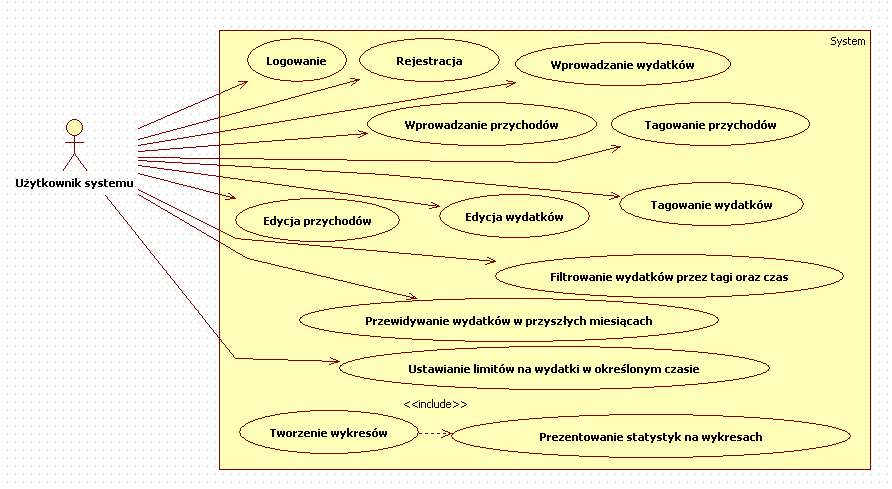
\includegraphics[scale=0.7]{images/use_case.png}
  \caption{Diagram przypadków użycia}
\end{figure}
\subsection{Projekt bazy danych}
Jak wyżej zostało napisane baza danych to Microsoft SQL Server 2012 Express LocalDB
Poniżej projekt bazy danych.
\subsection{Diagramy przedstawiające zależności między tabelami}
\begin{figure}[H]
  \centering
  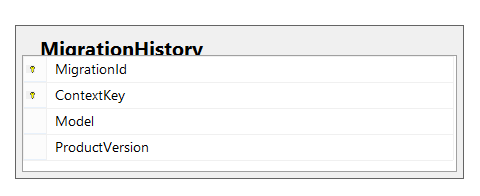
\includegraphics[scale=0.5]{images/db2.png}
  \caption{Tabela migracyjna}
\end{figure}
\begin{figure}[H]
  \centering
  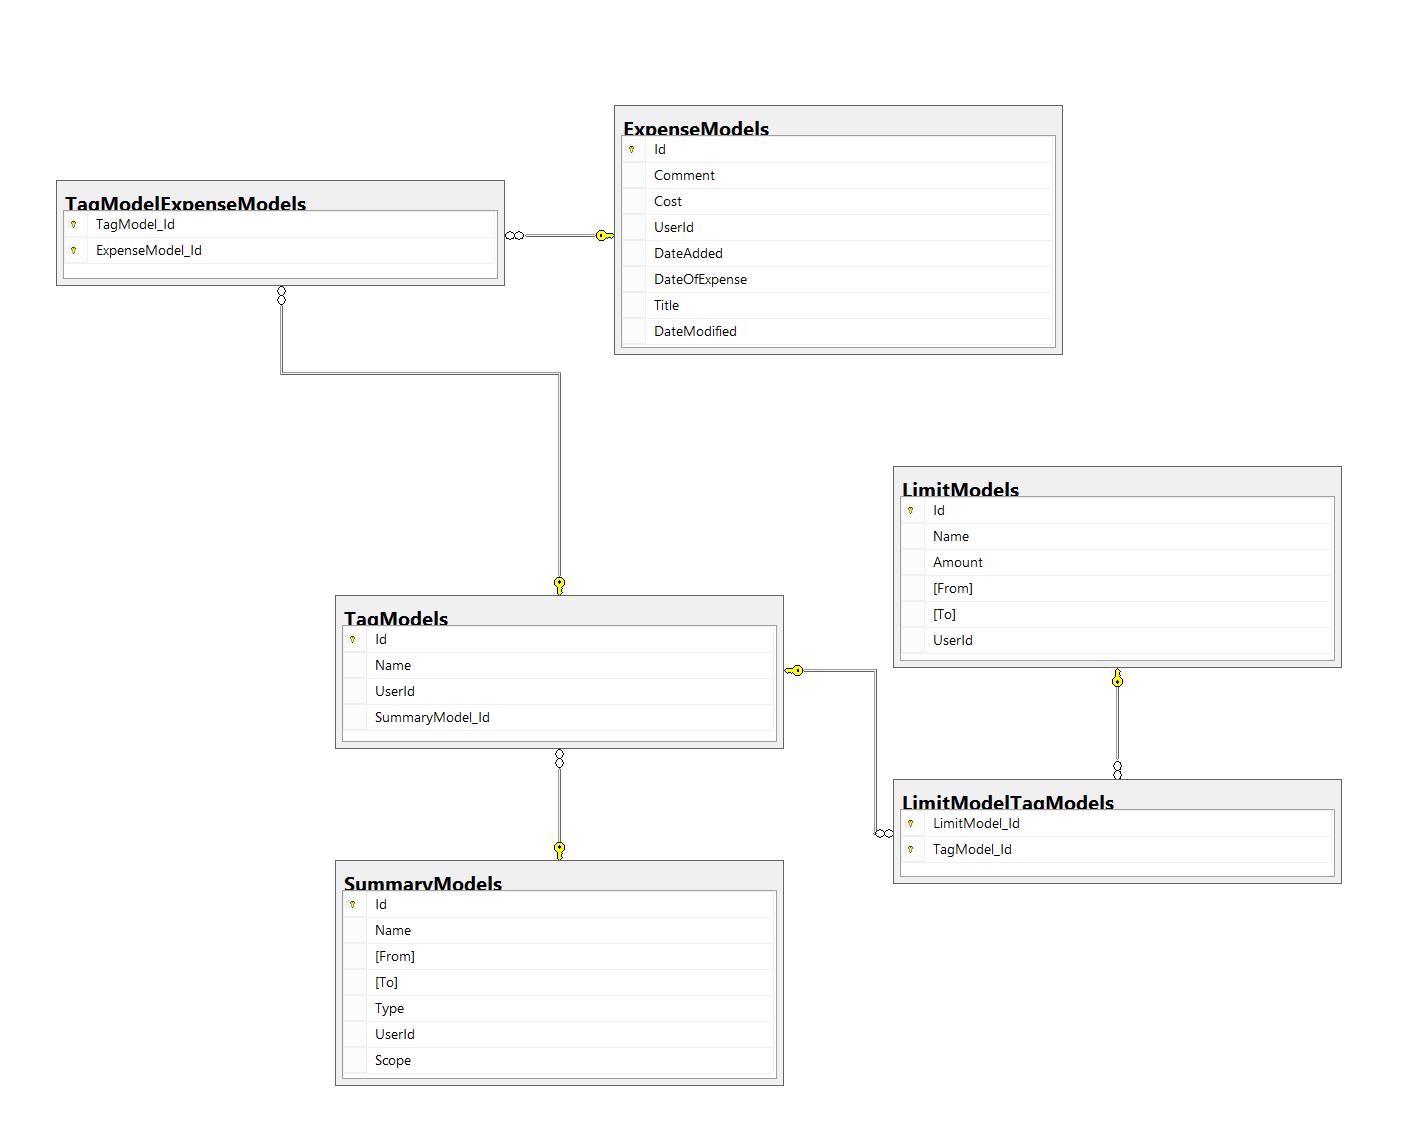
\includegraphics[scale=0.3]{images/db1.png}
  \caption{Tabele aplikacji}
\end{figure}
\begin{figure}[H]
  \centering
  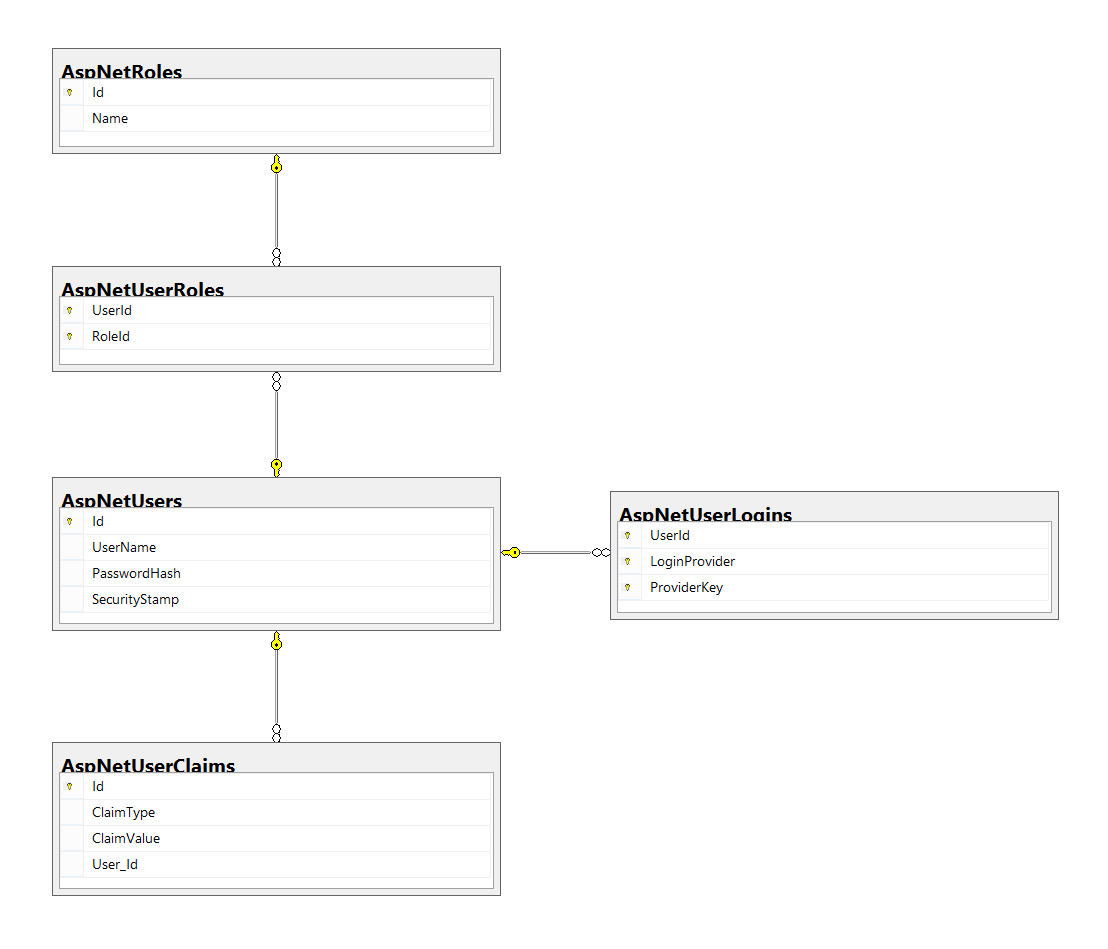
\includegraphics[scale=0.5]{images/db3.png}
  \caption{Tabele autoryzacyjne}
\end{figure}
\subsection{Opis tabel}
\paragraph[short]{ExpenseModels}
Przechowuje wydatki i przychody
\begin{itemize}
  \item Id int IDENTITY (Identyfikator)
  \item Comment nvarchar(max) (Komentarz)
  \item Cost decimal(18,2) (Wartość wydatku/przychodu)
  \item UserId nvarchar(max) (Identyfikator użytkownika)
  \item DateAdded datetime (Data dodania wydatku/przychodu)
  \item DateOfExpense datetime (Data wydatku/przychodu wprowadzona przez użytkownika)
  \item Title nvarchar(max) (Nazwa wydatku)
  \item DateModified datetime (Data modyfikacji wydatku/przychodu)
\end{itemize}
\paragraph[short]{LimitModels}
Przechowuje dane wyzwań
\begin{itemize}
  \item Id int IDENTITY (Identyfikator)
  \item Name nvarchar(max) (Nazwa wyzwania)
  \item Amount decimal(18,2) (Wartość wyzwania)
  \item From datetime (Data, od której zaczyna się wyzwanie)
  \item To datetime (Data, do której trwa wyzwanie)
  \item UserId nvarchar(max) (Identyfikator użytkownika)
\end{itemize}
\paragraph[short]{LimitModelTagModels}
Tabela łącząca tabele wyzwań z etykietami
\begin{itemize}
  \item LimitModelId int (Id wyzwania)
  \item TagModelId int (Id etykiety)
\end{itemize}
\paragraph[short]{SummaryModels}
Przechowuje dane podsumowań
\begin{itemize}
  \item Id int IDENTITY (Identyfikator)
  \item Name nvarchar(max) (Nazwa podsumowania)
  \item From datetime (Data, od której zaczyna się wyzwanie)
  \item To datetime (Data, do której trwa wyzwanie)
  \item Type int (Typ podsumowania)
  \item Scope int (Zasięg podsumowania np. roczne, miesięczne itd.)
  \item UserId nvarchar(max) (Identyfikator użytkownika)
\end{itemize}
\paragraph[short]{SummaryModelTagModels}
Tabela łącząca tabele podsumowań z etykietami
\begin{itemize}
  \item SummaryModelId int (Id podsumowania)
  \item TagModelId int (Id tagu)
\end{itemize}
\paragraph[short]{TagModelExpenseModels}
Tabela łącząca tabele wydatków/przychodów z etykietami
\begin{itemize}
  \item ExpenseModelId int (Id wydatku/przychodu)
  \item TagModelId int (Id tagu)
\end{itemize}
\paragraph[short]{TagModels}
Tabela przechowująca etykiety
\begin{itemize}
  \item Id int IDENTITY (Identyfikator)
  \item Name nvarchar(max) (Nazwa etykiety)
  \item UserId nvarchar(max) (Identyfikator użytkownika)
\end{itemize}
Pozostałe tabele są wykorzystywane przez standardowy mechanizm autentykacji ASP.NET MVC.
\section{Implementacja systemu}
W poniższym rozdziale przedstawione zostały liczne technologie, wzorce oraz zagadnienia. Dodatkowo zawiera on przykładowe kody źródłowe programu, które prezentują różne funkcjonalności.\\ W celu zaprezentowania widoków aplikacji załączone zostały zrzuty ekranów poszczególnych zakładek wraz z opisem.
\subsection{Opis technologii}
\subsubsection{Zagadnienia}
\paragraph{SPA - Single Page Application}
Jest to koncepcja, która mówi, że strona powinna być załadowana raz, a każde przejście na kolejną stronę ma być wykonywane asynchronicznie. Wszystkie zmiany strony są pokazywane przez modyfikację drzewa DOM w dokumencie HTML. Uzasadnieniem tego typu stron są rosnące doświadczenia użytkownika przy korzystaniu z aplikacji (User Experience), a także zminimalizowanie transferu danych między przeglądarką a serwerem, przez co czas odpowiedzi serwera jest zdecydowanie szybszy, a użytkownik szybciej zobaczy efekt. Koncepcja wiele czerpie z najnowszych technologii jakimi są HTML5, CSS3, JavaScript, AJAX.
\paragraph{MVC}
Złożony wzorzec architektoniczny służący do organizowania struktury aplikacji posiadających interfejsy graficzne. Wykorzystuje on 3 proste wzorce jakimi są Strategia, Obserwator, Kompozyt.\linebreak
MVC zakłada podzielenie aplikacji na poniżej wymienione częście składowe:
\begin{itemize}
  \item Model - dane wymagane do utworzenia Widoku
  \item Widok - opisuje jak przedstawić część modelu użytkownikowi
  \item Kontroler - agreguje dane z wielu modeli i przygotowuje je aby przekazać do widoku
\end{itemize}
\paragraph{Logowanie tokenowe}
Logowanie to działa na podobnej zasadzie jak logowanie przy pomocy ciasteczek, lecz znosi pewne ograniczenia jakie wcześniej wspomniany i najpopularniejszy w dzisiejszych czasach system identyfikacji sesji posiadał. Użytkownik, który chce się zalogować wpisuje swój login i hasło, na których podstawie jest generowany token (identyfikator sesji), który z kolei podajemy przy każdym wymagającym autentykacji żądaniu do serwera (poprzez dodanie w nagłówku żądania HTTP pola \verb|Authetication: Bearer <token>|). Token jest wydawany jedynie\\ na określony czas i służy do autentykacji tylko dla jednego użytkownika. Jedną z zalet tego logowania jest to, że możemy w aplikacjach SPA zalogować się bez odświeżenia strony i dodatkowo aplikacje klienckie możemy ``hostować'' na innej domenie. Nowoczesne strony wykorzystują już tego typu logowanie, idealnym przykładem jest protokół OAuth 2, który wykorzystują liczne strony:
\begin{itemize}
  \item Facebook
  \item Google+
  \item Twitter
\end{itemize}
\begin{figure}[H]
  \centering
  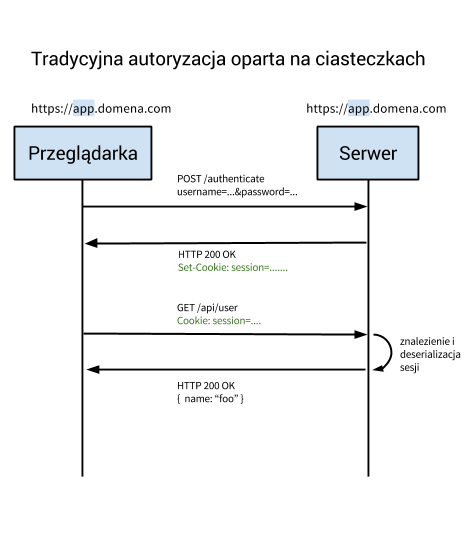
\includegraphics[scale=0.355]{images/tokenAuth1.png}
  \caption{Diagram przepływu dla logowania tradycyjnego}
\end{figure}
\begin{figure}[H]
  \centering
  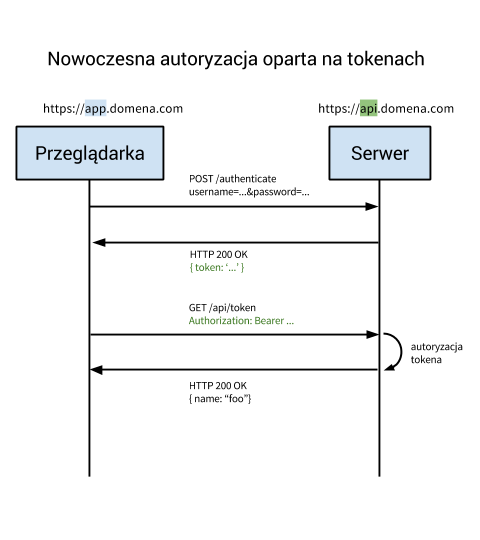
\includegraphics[scale=0.355]{images/tokenAuth2.png}
  \caption{Diagram przepływu dla logowania tokenowego}
\end{figure}
\subsubsection{Technologie}
Aplikacja została podzielona na 2 części logiczne, którymi są:
\begin{itemize}
  \item Serwer
  \item Klient
\end{itemize}
Każda z nich używa innych technologii, ponieważ działają w różnych środowiskach np. klient pracuje jedynie w przeglądarce.
\paragraph{Serwer}
Został napisany w języku C\# wykorzystując ASP.NET MVC 5 i ASP.NET Web Api 2. Statyczne pliki są udostępniane przy pomocy MVC, a reszta serwera została udostępniona w formie Web Service'u.\\ Silnik bazy danych, który został wykorzystany jest to Microsoft SQL Server 2012 w wersji Express LocalDB. Cała baza danych została zaprojektowana i wygenerowana przy pomocy Entity Framework 6, który także wspomaga wykonywanie zapytań do bazy danych. Zapytania w tej bibliotece nie wykonuje się bezpośrednio przy pomocy języka strukturalnego SQL, lecz pisząc kod i operując na encjach, a zapytania są generowane w locie. Wielką zaletą tego typu rozwiązania jest możliwość przeniesienia aplikacji na inny silnik bazy danych bez zmiany jakiegokolwiek fragmentu kodu. Jedyną rzeczą, którą trzeba będzie wykonać to zmienić parametry połączenia. Jest to typowe rozwiązanie mapowania obiektowo-relacyjnego w skrócie ORM.
\paragraph{Klient}
Klient został zaimplementowany przy pomocy biblioteki AngularJS. Jest to narzędzie napisane w JavaScript, które umożliwa tworzenie aplikacji za pomocą wzorca projektowego MVC,\\ a także ułatwia tworzenie według koncepcji Single Page Application.\\ Interfejs graficzny wykorzystuje bibliotekę Bootstrap, która nie tylko ładnie i schludnie wygląda, lecz przy zastosowaniu pewnych reguł zapewnia nam kompatybilność z innymi urządzeniami tj. telefony komórkowe, tablety, czytniki itd. Tego typu zgodność jest nazywana Responsive Web Desing i jest coraz częściej stosowana w Internecie.\\ Wykresy są tworzone przy pomocy HighCharts.js, dzięki czemu w łatwy sposób się je generuje.\\ Aplikacja została napisana modułowo i każdy takich modułów da się przetestować testami jednostkowymi, a wszystko dzięki narzuconemu schematowi przez AngularJS.
\subsection{Omówienie kodów źródłowych}
\subsubsection{Serwer}
\lstset{style=sharpc}
\lstinputlisting[caption=Mapowanie ścieżek routingu, label={lst:routeConfig}]{sources/server/routeConfig.cs}
\par Powyższy kod służy do nauczenia serwera IIS interpretowania ścieżek adresu wpisywanych przez użytkownika. Pierwsza linijka metody \verb|RegisterRoutes| jest wymagana przez rozszerzenie Elmah, które służy do monitorowania aplikacji. Mówi ona, że ten typ adresów ma być przez naszą aplikację ignorowany. Adresy, które spełniają ten warunek to np. \verb|http://domena.pl/elmah.axd| lub \verb|http://domena.pl/elmah.axd/1234|. Kolejna użyta metoda jest napisana na potrzeby aplikacji metoda, która linkuje każdy z adresów pasujących do wyrażeń z pierwszego argumentu metody \verb|MapHtml5Routes| na controller podany w drugim parametrze. Zabieg ten jest wymagany przez router Angular'a, który w aplikacji działa w HTML5Mode i daje dostęp do adresów URL bez poprzedzania każdej ścieżki znakiem \verb|#|. Kod metody przedstawia Listing \ref{lst:mapHtml5Routes}. Podobnym plikiem jest \verb|AngularPlanner/AngularPlanner/App_Start/WebApiConfig.cs|, który ustawia ścieżki routingu dla Web Service'u RESTowego.
\lstinputlisting[caption=Metoda MapHtml5Routes, label={lst:mapHtml5Routes}]{sources/server/mapHtml5Routes.cs}
\par W pliku \verb|AngularPlanner/AngularPlanner/App_Start/BundleConfig.cs| są tworzone paczki plików JavaScript, które na środowisku produkcyjnym są zmiejszone i zoptymalizowane. Zaletą tego rozwiązania są mniejsze transfery danych i szybszy kod po stronie przeglądarki.\par Plik \verb|AngularPlanner/AngularPlanner/App_Start/Startup.Auth.cs| zawiera konfigurację mechanizmu autentykacji tokenowej dla naszej aplikacji. Ponadto istnieje możliwość dodania opcji logowania przez Facebook i Google+.\par Katalog \verb|Controllers| zawiera klasy kontrollerów. Przedewszystkim są tam kontrolery Web Api\\ 2, lecz jest tam jeden, który posiada tylko akcję, która z kolei zwraca użytkownikowi widok podany na Listingu \ref{lst:homeIndexView}.
\lstinputlisting[caption=Widok zwracany przez akcję \texttt{Index} kontrolera \texttt{Home}, label={lst:homeIndexView}, language=HTML]{sources/server/homeIndexView.cshtml}
\par Pozostałe kontrollery są do siebie podobne, a kod wybranego z nich można zobaczyć poniżej.
\lstinputlisting[caption=Kontroller ExpensesController, label={lst:expensesController}]{sources/server/expensesController.cs}
\par Klasa kontrollera dziedziczy po klasie abstrakcyjnej ApiController, by mogłabyć rozpoznana przez mechanizm refleksjii jako kontroller Web Api 2 i dodatkowo uzyskać dostęp do kilku przydatnych metod charakterystycznych dla tego typu kontrolerów. Trochę wyżej są 2 atrybuty. \verb|Authorize| oznacza, że dostęp do kontrolera mają jedynie zalogowani użytkownicy, a atrybut \verb|ElmahHandleErrorApi| infromuje bibliotekę Elmah, że ma przechwytywać wyjątki z tego kontrollera. W konstruktorze mamy tworzenie instacji połączenia z bazą danych przy pomocy Entity Framework. W klasie mamy zaimplementowane wszystkie akcje CRUD, czyli Create (metoda \verb|Post|), Read (metody \verb|GetListByDate|, \verb|GetListByTag|, \verb|GetList|, \verb|GetSingle|), Update (metoda \verb|Put|) i Delete (metoda \verb|Delete|). Linia nr 100 przedstawia przykładowe zapytanie do bazy. Odpowiada to zapytaniu w SQLu
\begin{verbatim}
SELECT TOP 1 * FROM dbo.ExpenseModels WHERE UserId = <UserId> AND Id = <Id>
\end{verbatim}
Kolejnym dobrym przykładem zapytania są linie od 78 do 85. Metoda Include wykonuje\\ \verb|LEFT OUTER JOIN| z tabelą \verb|TagsModels|, znowu metoda OrderByDescending dodaje sortowanie po \verb|DateOfExpense| (\verb|ORDER BY DateOfExpense DESC|), \verb|Skip| opuszcza liczbę wpisów podanych w parametrze, a \verb|Take| pobiera 20 rekordów. Ważnym elementem tego zapytania jest także \verb|ToListAsync|. Do póki nie użyjemy tej metody zapytanie nie zostanie wykonane, a jedynie przygotowane. Po wykonaniu zapytania (zmaterializowaniu) dane są typu \verb|List|, a wcześniej były \verb|IQueryable|.

\par Pliki w katalogu \verb|Models| z wyłączeniem \verb|AngularPlannerContext| są to pliki reprezentujące bazę danych. Każda klasa reprezentuje rzeczywistą tabelę w bazie. Dla przykładu została przedstawiony model \verb|Expense| w Listingu \ref{lst:expenseModel}
\lstinputlisting[caption=Model ExpenseModel, label={lst:expenseModel}]{sources/server/expenseModel.cs}
Atrybut \verb|Key| oznacza pole, które jest typu \verb|PRIMARY KEY|. Pole \verb|Tags| jest to tak naprawdę odwołanie do tabeli \verb|TagsModels|. Entity Framework sam stwierdza jakiego typu relacjami mają być połączone tabele w bazie danych (jeden-do-wielu, wiele-do-wielu itd.). Pola \verb|Nullable<DateTime>| oznaczają, że to nie są wymagane i mogą mieć wartość \verb|NULL| w bazie.
\subsubsection{Klient}
\lstset{language=JavaScript}
\par Cały kod aplikacji został zorganizowany według rekomendowanej przez Angulara struktury katalogów ~\cite{angular:structure}.
\par Przy asynchronicznych akcjach jest wykorzystywana okrojona biblioteka \verb|Q.js| ~\cite{lib:q} zaimplementowana w Angularze. Implementuje ona ustandaryzowany system obietnic Promises/A+ ~\cite{doc:promises}
\lstinputlisting[caption=Plik konfiguracyjny systemu budującego Grunt, label={lst:gruntfile}]{sources/client/Gruntfile.js}
\par Kod przestawiony na powyższym listingu jest plikiem konfiguracyjnym dla systemu do automatyzacji pewnych zadań \verb|Grunt|. Można go porównać do \verb|Makefile|, ponieważ jest to narzędzie tego typu, lecz istnieje do niego wiele rozszerzeń, które ułatwiają pracę. Powyżej definiujemy 3 zadania: default, test, dev. Każdy z nich można uruchomić za pomocą polecenia \verb|grunt <nazwa_zadania>|. Dev i default nasłuchują katalogi z plikami \verb|*.js|, \verb|*.css|, \verb|*.html|, a następnie robią wstępną kompilację, aby kod napisany był możliwy do pomniejszenia ~\cite{angular:minSafe} i sprawdzany pod względem poprawności składni. Także informowana jest przeglądarka o zmianach, których następstwem jest automatyczne odświeżenie okna przeglądarki. Jest to czynność, która znacznie przyspiesza proces wytwarzania oprogramowania.
\par Plik z Listingu \ref{lst:appJs} jest plikiem startowym aplikacji. Definiuje się tutaj jakie moduły wchodzą w skład aplikacji i konfiguruje środowisko do dalszej pracy. W tym przypadku został włączony \verb|html5Mode| i domyślne przekierowanie na stronę \verb|domena.pl/statistics|. W pliku z Listingu \ref{lst:homeIndexView} jest podłączenie aplikacji do drzewa DOM za pomocą \verb|<body ng-app="app">|.
\lstinputlisting[caption=Plik startowy aplikacji, label={lst:appJs}]{sources/client/app.js}
Mechanizm autentykacji po stronie klienta został napisany na podstawie książki ~\cite{angular:bookMastering}. Jest on podzielony na trzy moduły. Pierwszy z nich przedstwiony na Listingu \ref{lst:authInterceptor} pośredniczy przy żądaniach \linebreak i odpowiedziach dodając \verb|Token| w nagłówkach żądania, jeśli jest on zapisany w \verb|localStorage| przeglądarki. Jeśli \verb|Token| wygaśnie lub jest nieprawidłowy, serwer poinformuje klienta statusem kodu \verb|401 - Unauthorized| ~\cite{http:statuscodes}
\lstinputlisting[caption=Moduł pośredniczący przy żądaniach i odpowiedziach HTTP, label={lst:authInterceptor}]{sources/client/authInterceptor.js}
Kolejny przedstawiony na Listingu \ref{lst:authJs} moduł to udostępniający najważniejsze metody do autentykacji i sprawdzenia zalogowania użytkownika.
\lstinputlisting[caption=Moduł wystawiający interfejs do autentykacji, label={lst:authJs}]{sources/client/auth.js}
\par Udostępnia on metody \verb|login|, \verb|logout|, \verb|register|, \verb|isAuthenticated|. W przypadku \verb|login| serwer jest odpytywany czy użytkownik z takimi danymi logowania istnieje w bazie danych, jeżeli tak jest, to w odpowiedzi dostajemy \verb|Token| autoryzacyjny, który zostaje zapisany w pamięci przeglądarki.
\par Ostatnim z modułów odpowiedzialnych za logowanie jest przedstwiony poniżej. Sprawdza czy widoki mogą być pokazane użytkownikowi. Adresy końcowe dla autentykacji zostały zaczerpnięte z tutoriala ~\cite{server:tokenLogin}.
\lstinputlisting[caption=Moduł sprawdzający czy dany widok jest dostępny dla anonimowego użytkownika, label={lst:authCheckerJs}]{sources/client/authChecker.js}
\par Do wymiany danych używany jest mechanizm \verb|$resource| ~\cite{angular:$resource}. Przykład implementacji przedstawiony został na Listingu \ref{lst:summaryJs}. Udostępnia on łatwy interfejs do komunikacji z serwerem.
\lstinputlisting[caption=Tags Resouce, label={lst:summaryJs}]{sources/client/summaries.js}
\par Zastosowanie w/w mechanizmu jest podane w Listingu \ref{lst:tagsPickerJs}. Poprzez \verb|Tags.query(callback)| odpytujemy serwer o listę wszystkich etykiet na serwerze. Poprzez utworzenie nowej instancji tworzymy nową etykietę, a wywołując na nim metodę \verb|.$save(callback)| zapisujemy go na serwerze.
\lstinputlisting[caption=Dyrektywa <tags-picker />, label={lst:tagsPickerJs}]{sources/client/tagsPicker.js}
\par Warto także wspomnieć, że Listing \ref{lst:tagsPickerJs} tworzy nowy element HTMLa, który jest nazwany\\ \verb|<tags-picker />|. Definicja takiego elementu jest zawarta w liniach od 94 do 104. Parametr \verb|scope| nakazuje utworzyć obiekt podgląd, który jest obiektem dla tego elementu. Danymi źródłowymi są atrybuty dostarczone do elementu. Wartość \verb|'='| nakazuje zachować \verb|2-way data binding| ~\cite{angular:databinding} między widokiem, a kontrolerem dla tej właściwości. \verb|controller| wskazuje, który kontroler ma być wykorzystany. Jest on zaimplementowany wyżej. Parametr \verb|resrict| determinuje jakiego typu ma być dyrektywa ~\cite{angular:restrict}. Więcej o konfiguracjach można przeczytać ~\cite{angular:$compile}.
\par Metody i właściwości są udostępnianie widokowi przy pomocy \verb|$scope|. W kontrolerze jest kilka przykładów: \verb|$scope.delete = function(){}|, \verb|$scope.tags = []|. Także dla właściwości w \verb|$scope| udostępniony został mechanizm obserwowania zmian w tej własciwości. Jest to klasyczne zastosowanie wzorca \verb|Obserwator|. Istnieje też system wiadomości, w którym możemy nasłuchiwać na konkretną wiadomość (\verb|$scope.$on('tagsPicker:push')|) i je wysyłać w górę drzewa podglądów (\verb|$scope.$emit('tagsPicker:push')|) lub w dół (\verb|$scope.$emit('tagsPicker:push')|).
\lstinputlisting[caption=Widok dla dyrektywy <tags-picker />, label={lst:tagsPickerHTML}, language={HTML}]{sources/client/tagsPicker.html}
\par W widoku podpięte są metody na akcje. Dla przykładu można podać \verb|ng-click="delete($index)"|. Kliknięcie w element wywołuje tą metodę z kontrolera. Atrybut \verb|ng-repeat="tag in tagsList"| nakazuje powielić element, do którego jest podpięty tyle razy ile jest elementów w tablicy \verb|tagsList|.
\lstinputlisting[caption=Przykładowy kod podstrony, label={lst:expensesCtrl}]{sources/client/expensesController.js}
\par Na samej górze mamy definicje adresów, które prowadzą do podstrony. Każdy z nich ma podany widok i kontroler, przez które będzie obsługiwany adres. W właściwości są zależności, które są wymagane do przejścia na podstronę np. \verb|currentUser: authCheckerProvider.require| jest odpowiedzialny za autoryzację. Jeżeli, któraś z tych zależności nie zostanie spełniona to przejście nie zostanie wykonane, a sam \verb|$routeProvider| wyśle komunikat \verb|$routeChangeError| ~\cite{angular:$routeChangeError}. Poniżej mamy definicję samego kontrolera.
\subsection{Prezentacja systemu}
Poniżej został przedstawiony ekran logowania. Jest to także pierwszy ekran widziany przez użytkownika. Po zalogowaniu ma dostęp do swoich wykresów i wydatków. Jeżeli użytkownik nie ma konta może nacisnąć przycisk \verb|Rejestracja| i zostanie przeniesiony do widoku pokazanego na rysunku nr ~\ref{screen:register}.
\begin{figure}[H]
  \centering
  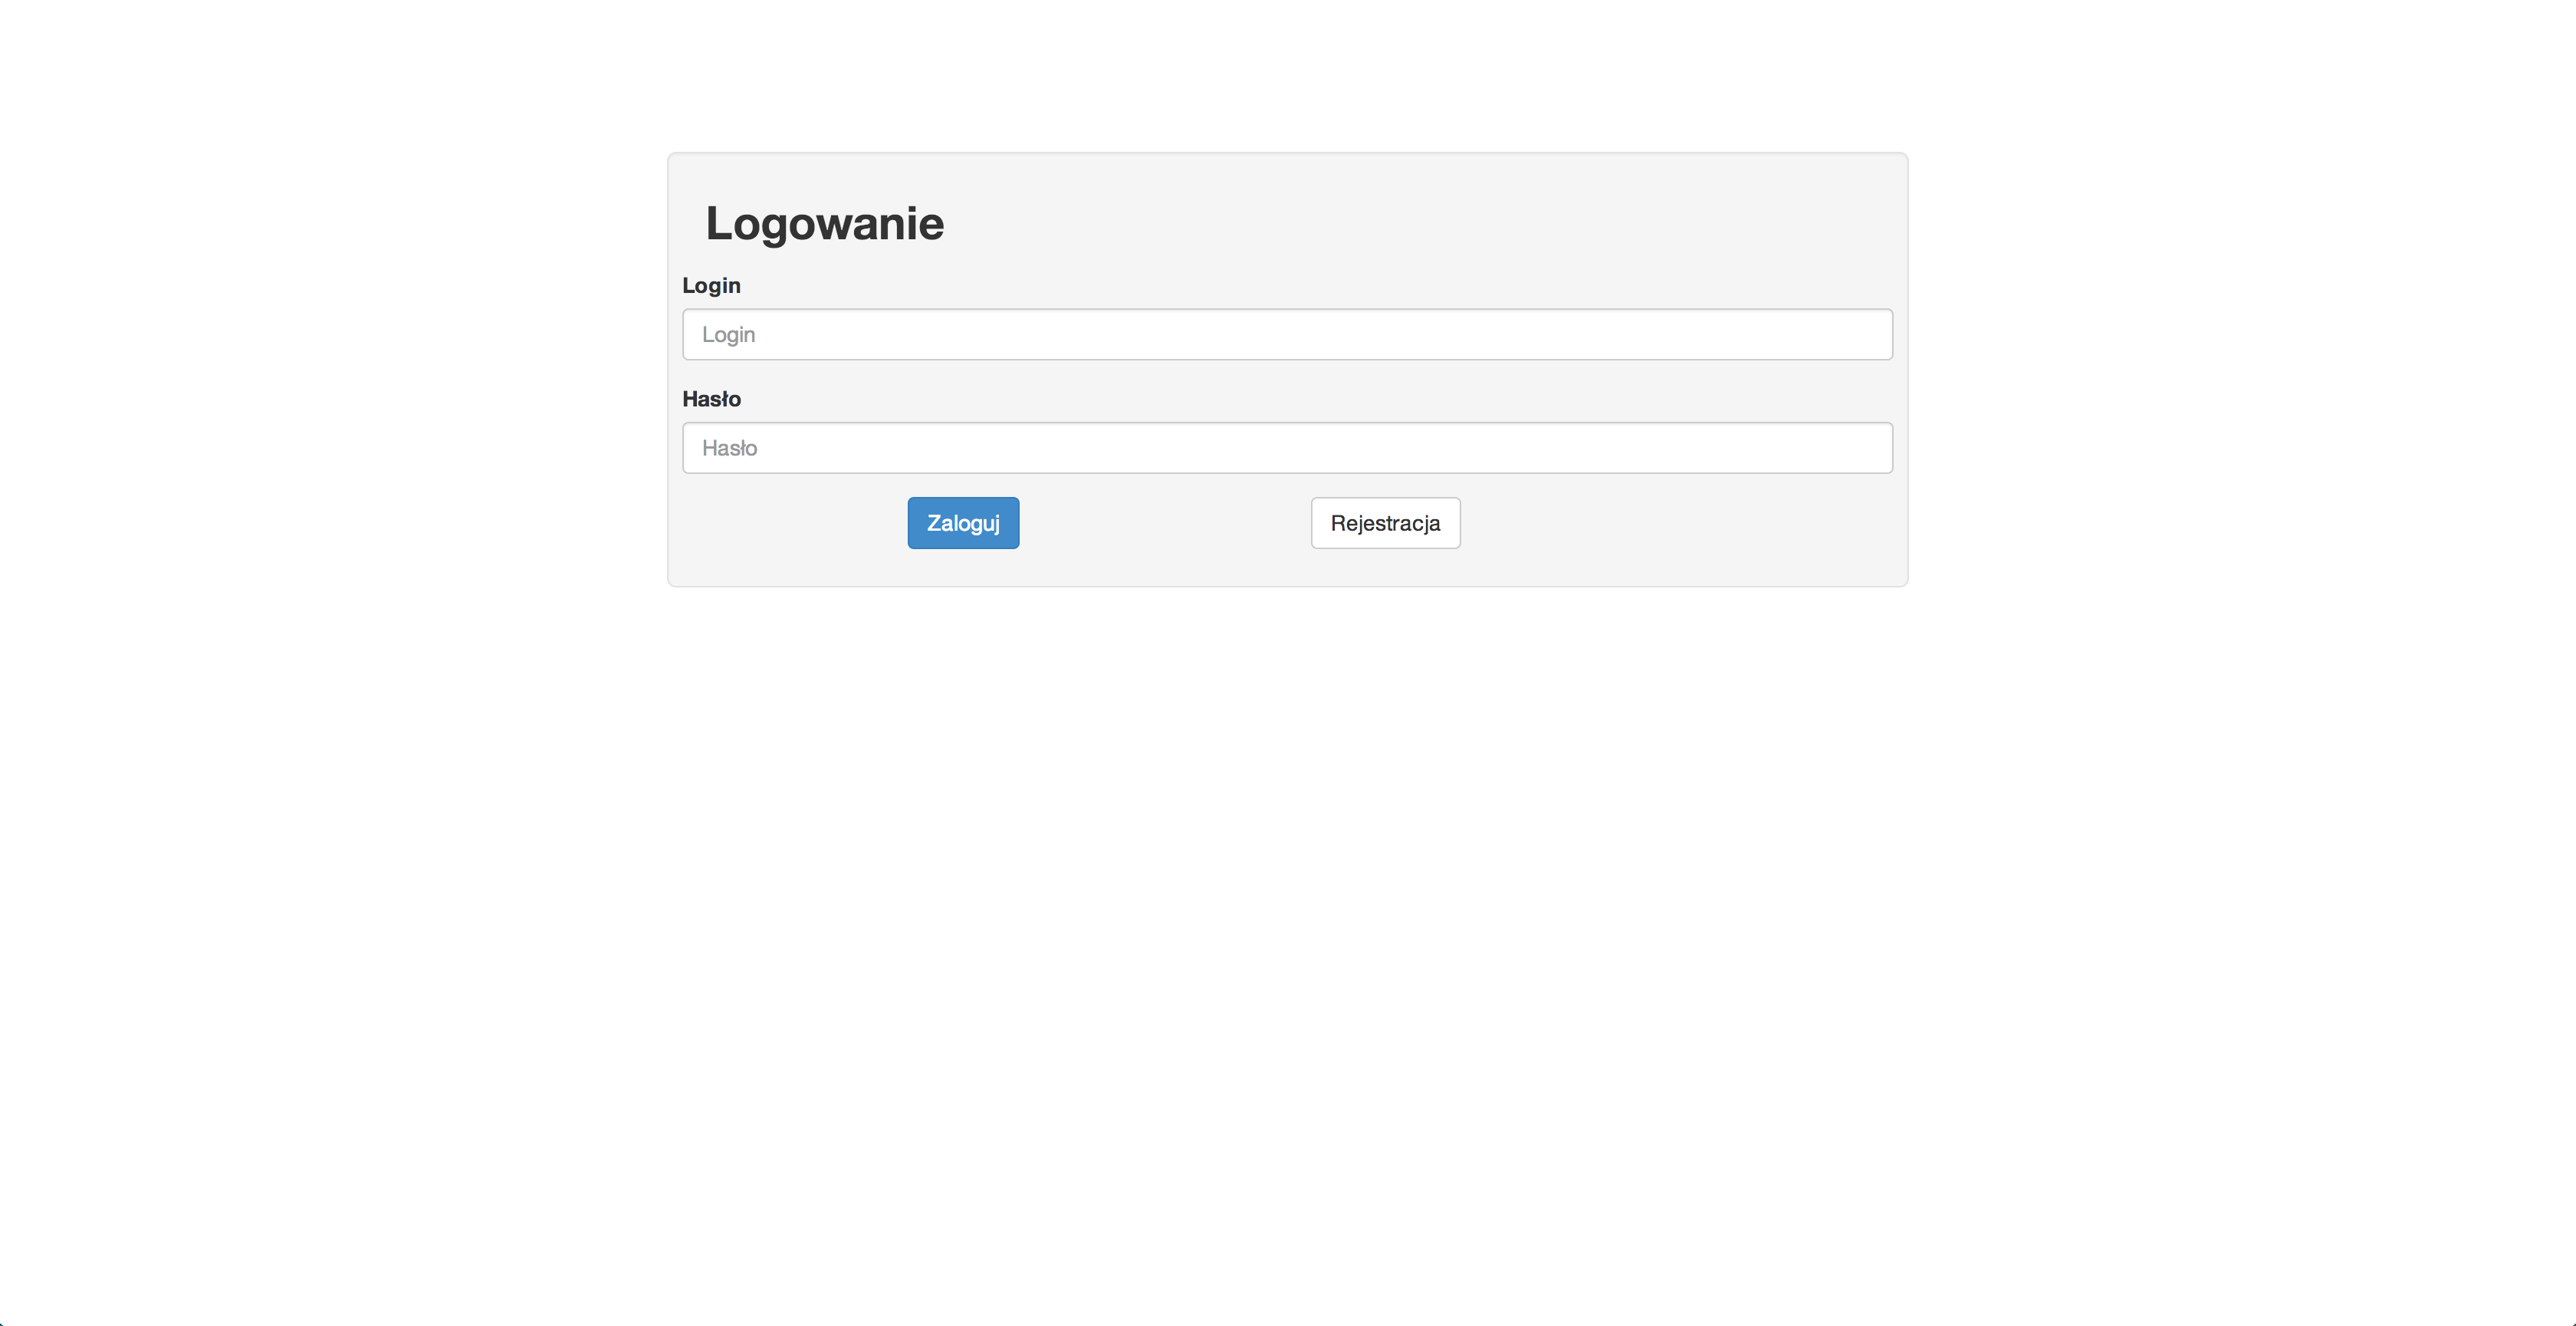
\includegraphics[scale=0.2]{images/screen_logowanie.png}
  \caption{Ekran logowania}
\end{figure}
Na rysunku nr ~\ref{screen:register} jest ekran rejestracji, którego pomocy możemy założyć nowe konto. Przyciskiem \verb|Logowanie| wracamy do ekranu logowania.
\begin{figure}[H]
  \centering
  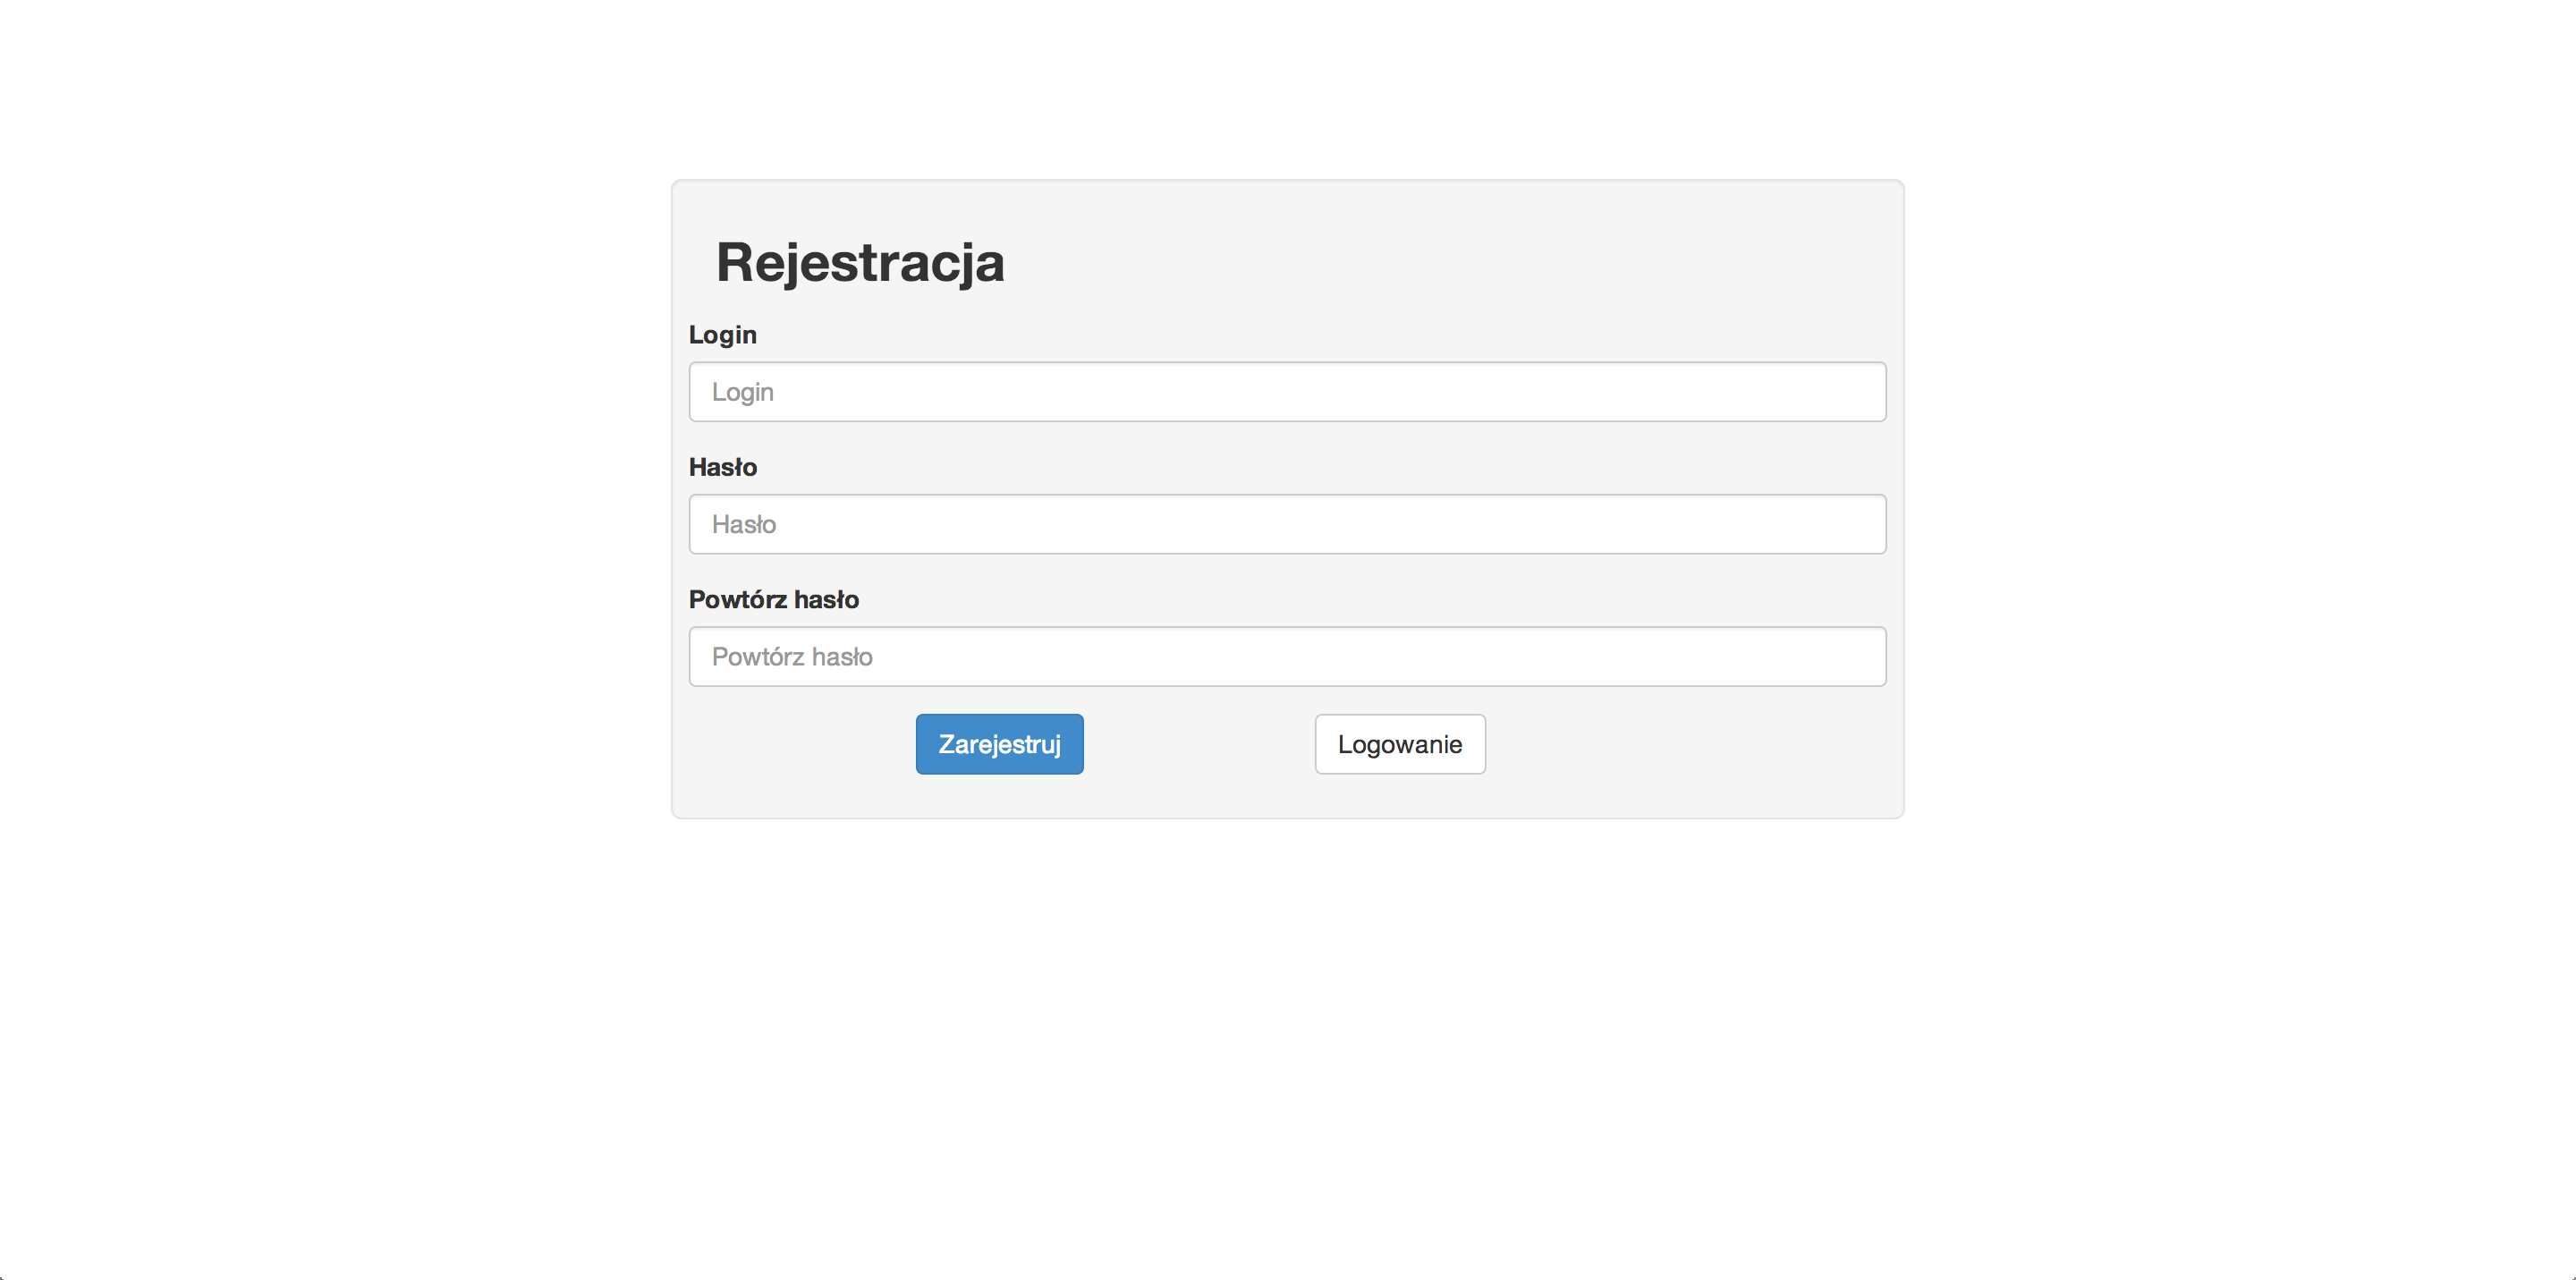
\includegraphics[scale=0.2]{images/screen_rejestracja.png}
  \caption{Ekran rejestracji}
  \label{screen:register}
\end{figure}
\par Na liście wszystkich wydatków i przychodów możemy dodawać nowe wydatki i przychody, a także usuwać i edytować istniejące. Aby dodać nowy wydatek trzeba skorzystać z formularza na górze i wprowadzić wszystkie wymagane dane. Dodatkowe dane można uzupełnić klikając na przycisk \verb|Więcej|. Ujawniają się wtedy etykiety do wyboru i komentarz do uzupełnienia.
\par Edycja elementu następuje po naciśnięciu niebieskiego przycisku z ikoną długopisa, po naciśnięciu którego pojawia się panel do edycji przedstawiony na rysunku nr ~\ref{screen:editExpense}. Znajdują się tam wszystkie opcje dostępne przy zakładaniu nowego elementu. Aby zapisać wydatek trzeba potwierdzić zmiany przez naciśnięcie \verb|Zapisz|.
\par Obok przycisku edycji znajduje się czerwony przycisk do usuwania.
\begin{figure}[H]
  \centering
  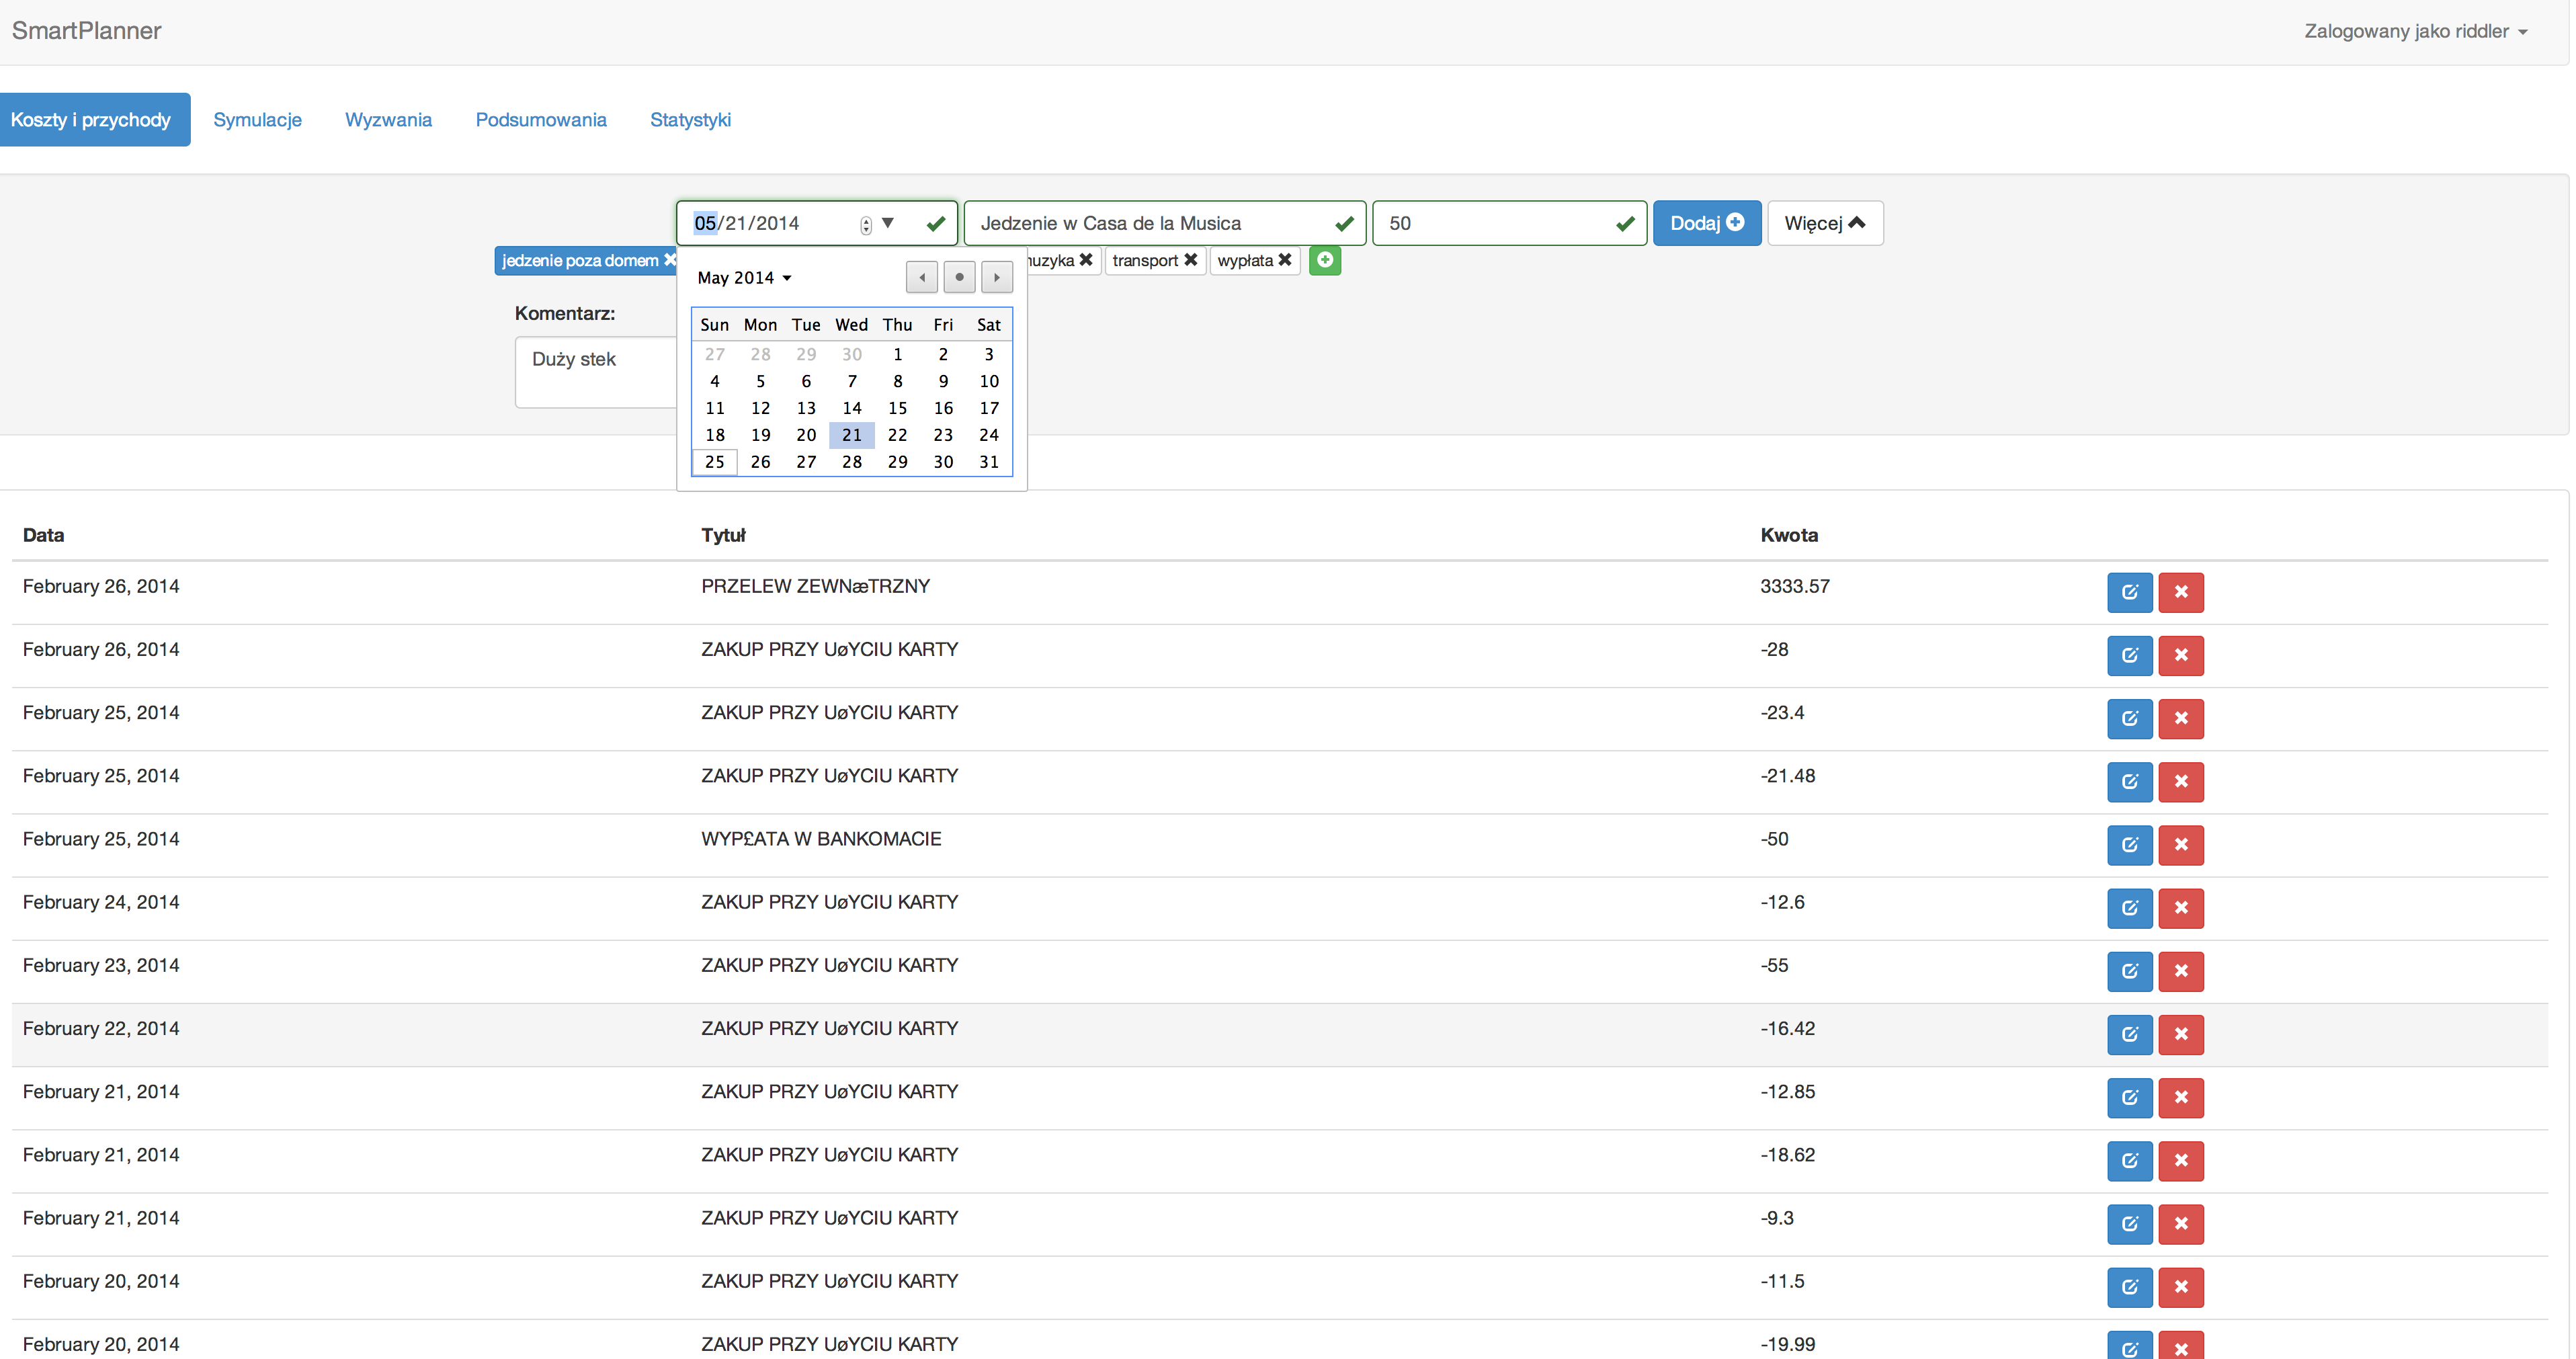
\includegraphics[scale=0.2]{images/screen_dodawaniewydatkow.png}
  \caption{Lista wydatków i dodawanie}
  \label{screen:listExpense}
\end{figure}
\begin{figure}[H]
  \centering
  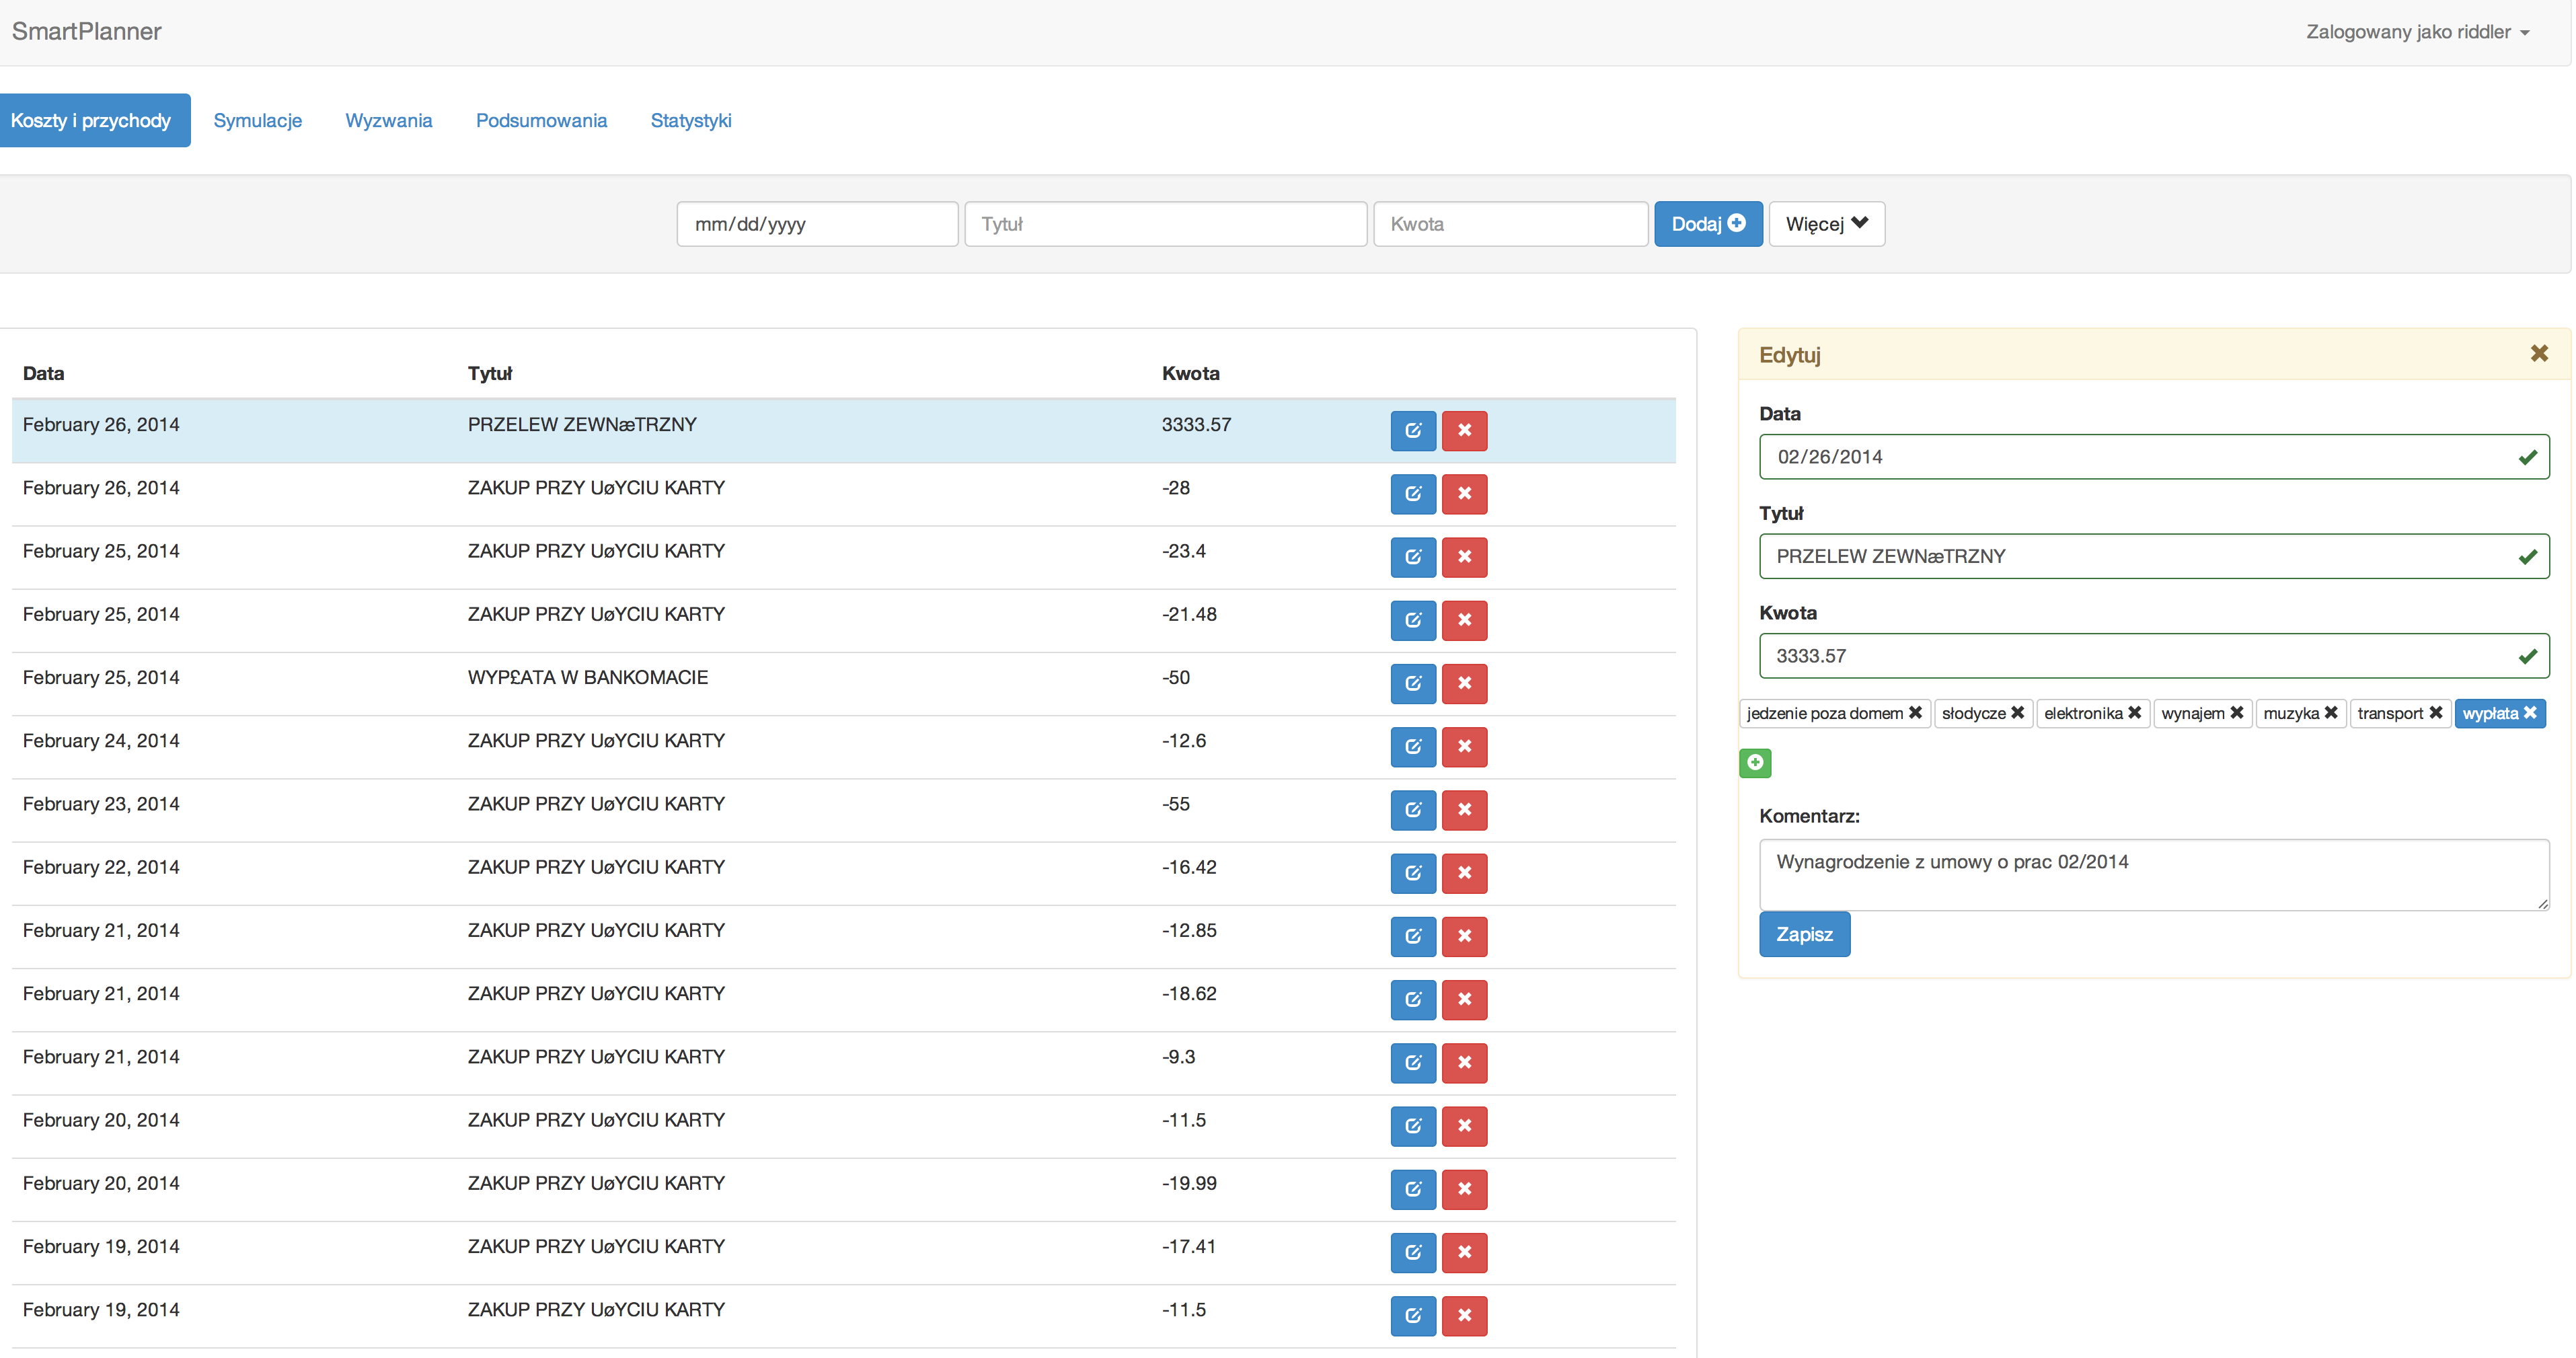
\includegraphics[scale=0.2]{images/screen_edycjaWydatku.png}
  \caption{Edycja wydatków}
  \label{screen:editExpense}
\end{figure}
\par Poniżej jest ekran do planowania wydatków. W panelu po prawej wprowadzamy planowany przychód i wydatek na przyszłe miesiące/dni/lata i na żywo jest przedstawiana zdolność do realizacji wyżej wymienionego planu. Na wykresie jest przedstawione kilka serii, lecz każdą można wyłączyć przez naciśnięcie etykiety serii w legendzie.
\begin{figure}[H]
  \centering
  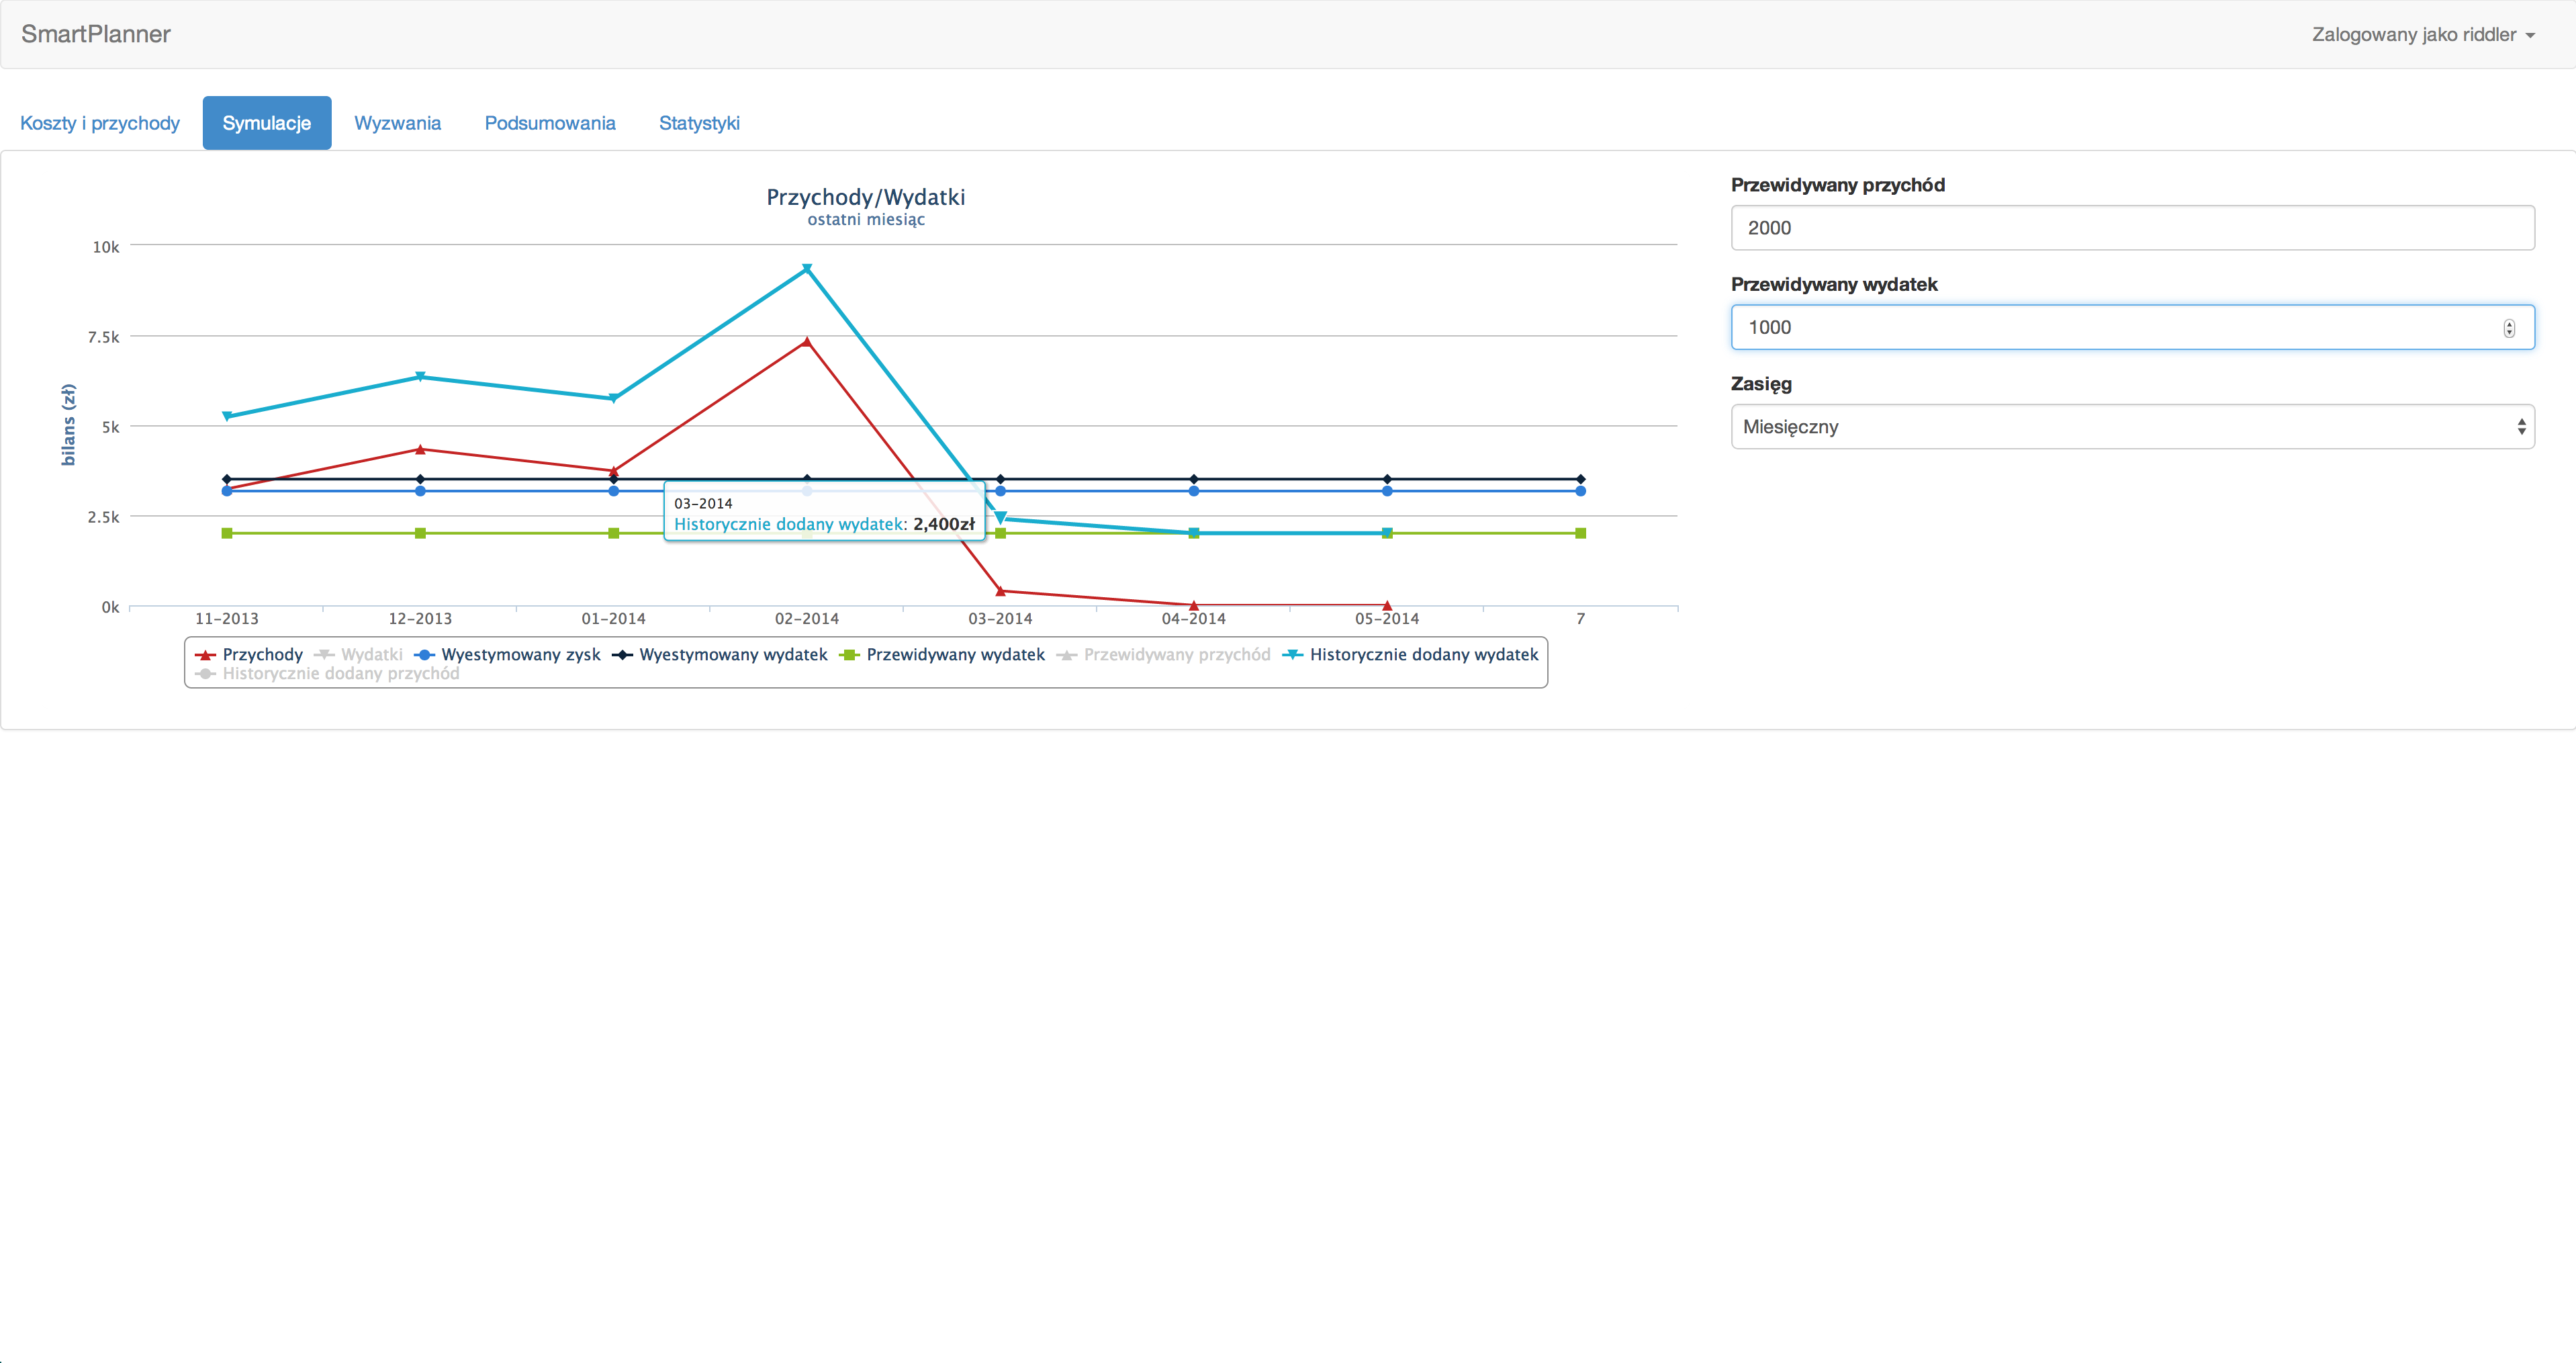
\includegraphics[scale=0.2]{images/screen_planowanieWydatkow.png}
  \caption{Planowanie wydatków}
\end{figure}
\par Podsumowania służą do tworzenia raportów. Można przykładowo stworzyć raport wydatków za ostatni miesiąc i przedstawić w formie wykresu. Przykład przedstwiony jest poniżej.
\par Dodawanie wydatku przedstawione na rysunku nr ~\ref{screen:addSummary} pozwala utworzyć podsumowanie. Aby przejść do tego widoku trzeba nacisnąć kafelek z ikoną plusa. Na tym widoku kiedy wybierzemy etykiety to aplikacja zawęzi wyszukiwanie wydatków do tych właśnie etykiet.
\par Edycja z rysunku ~\ref{screen:editSummary} działa analogicznie jak dodawanie.
\begin{figure}[H]
  \centering
  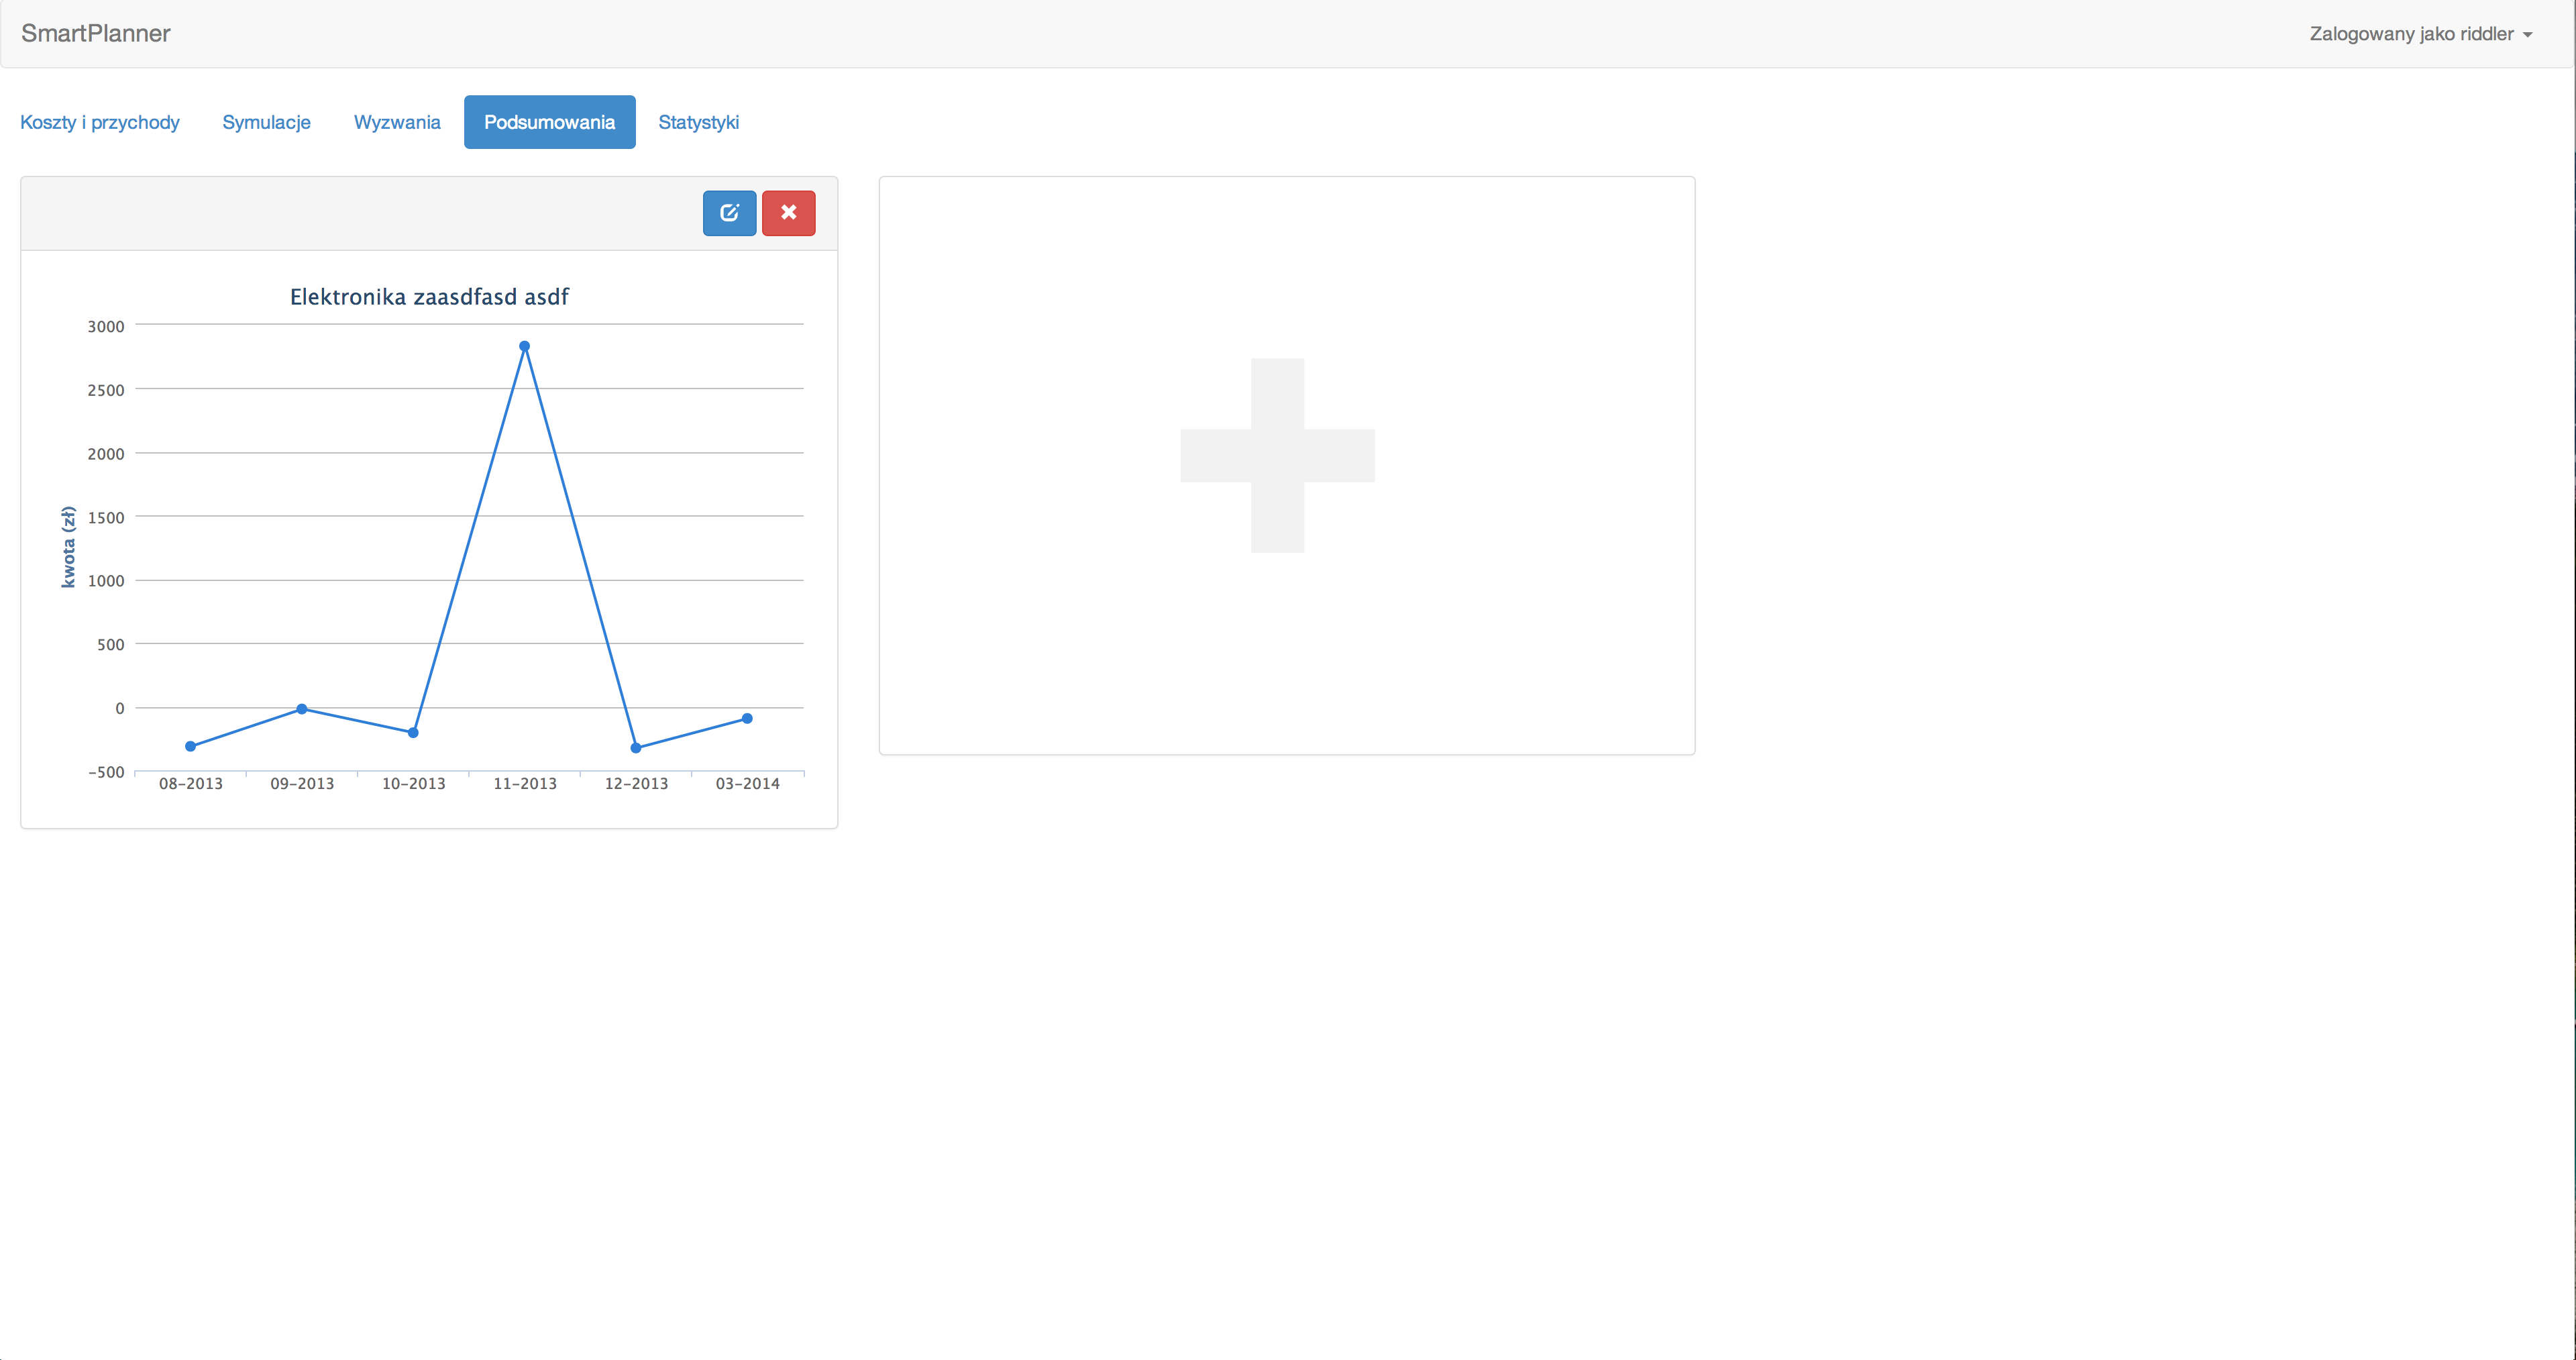
\includegraphics[scale=0.2]{images/screen_podsumowania.png}
  \caption{Lista podsumowań}
\end{figure}
\begin{figure}[H]
  \centering
  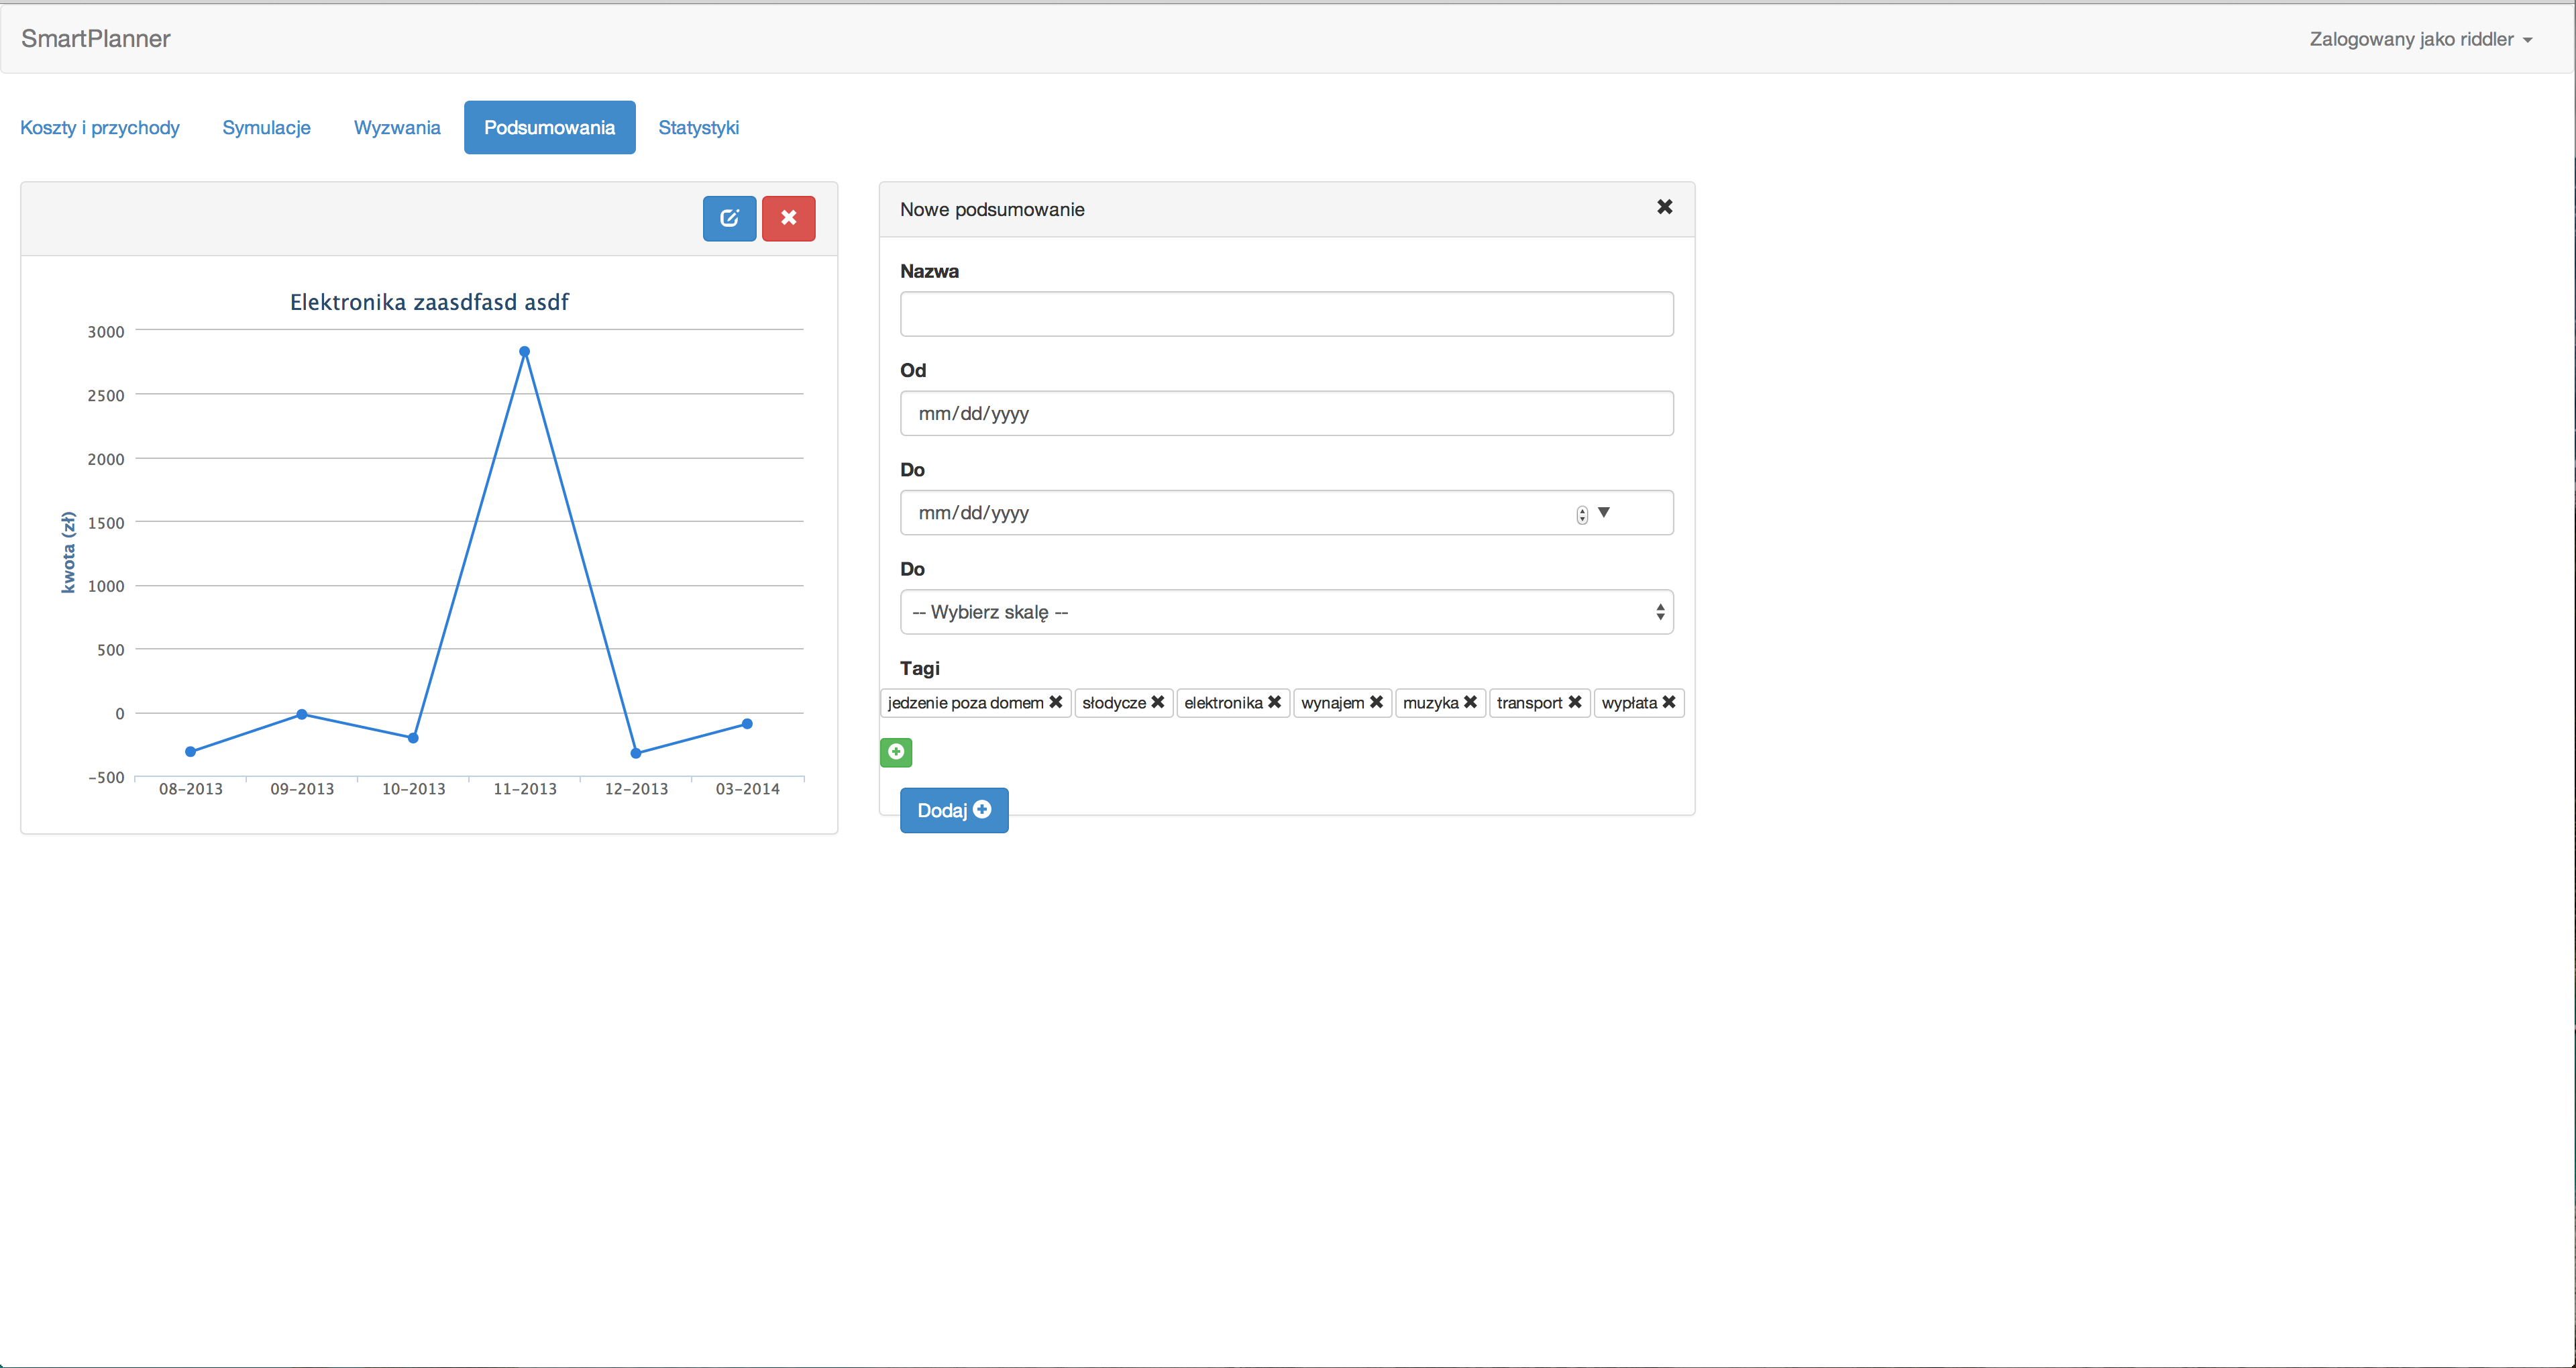
\includegraphics[scale=0.2]{images/screen_podsumowaniaDodaj.png}
  \caption{Dodawanie podsumowań}
  \label{screen:addSummary}
\end{figure}
\begin{figure}[H]
  \centering
  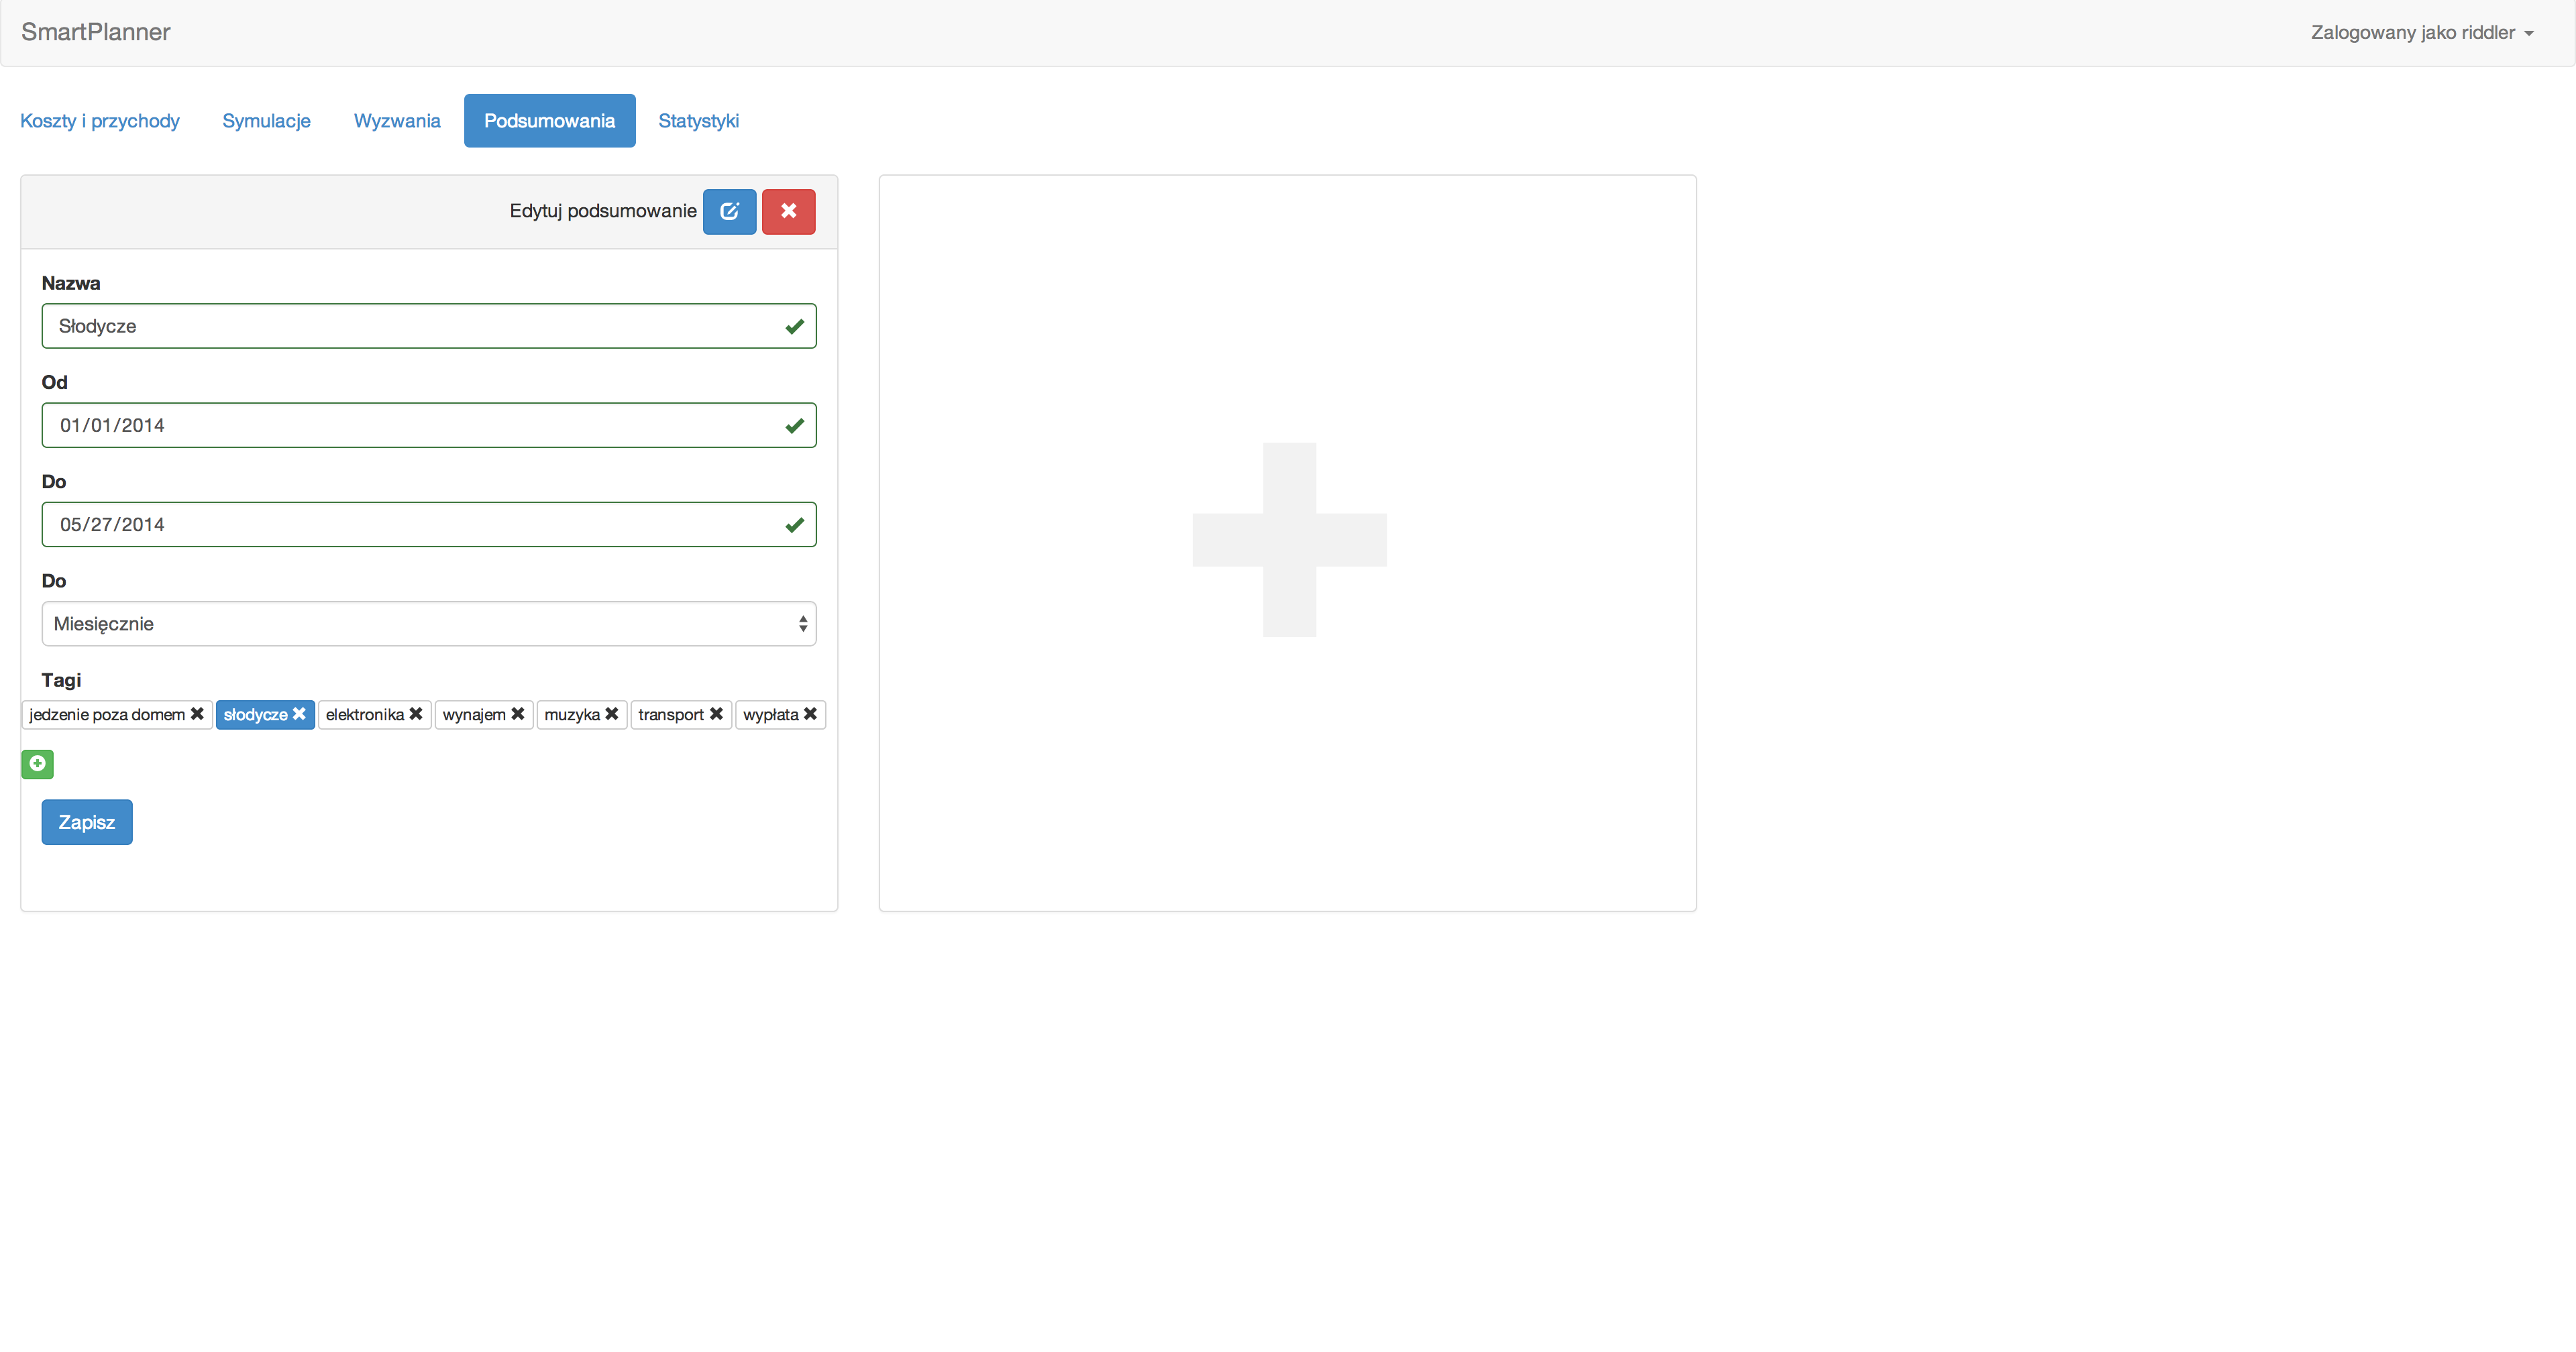
\includegraphics[scale=0.2]{images/screen_podsumowaniaEdycja.png}
  \caption{Edycja podsumowania}
  \label{screen:editSummary}
\end{figure}
\par Wyzwania służą do wyznaczania sobie celów na najbliższe miesiące. Pokazują aktualny stan wydanych pieniędzy na wydatki oznaczone wybranymi etykietami. Poniżej zrzuty z listy, edycji, dodawania, powodzenia w wykonaniu i niepowodzeniu wyzwania.
\begin{figure}[H]
  \centering
  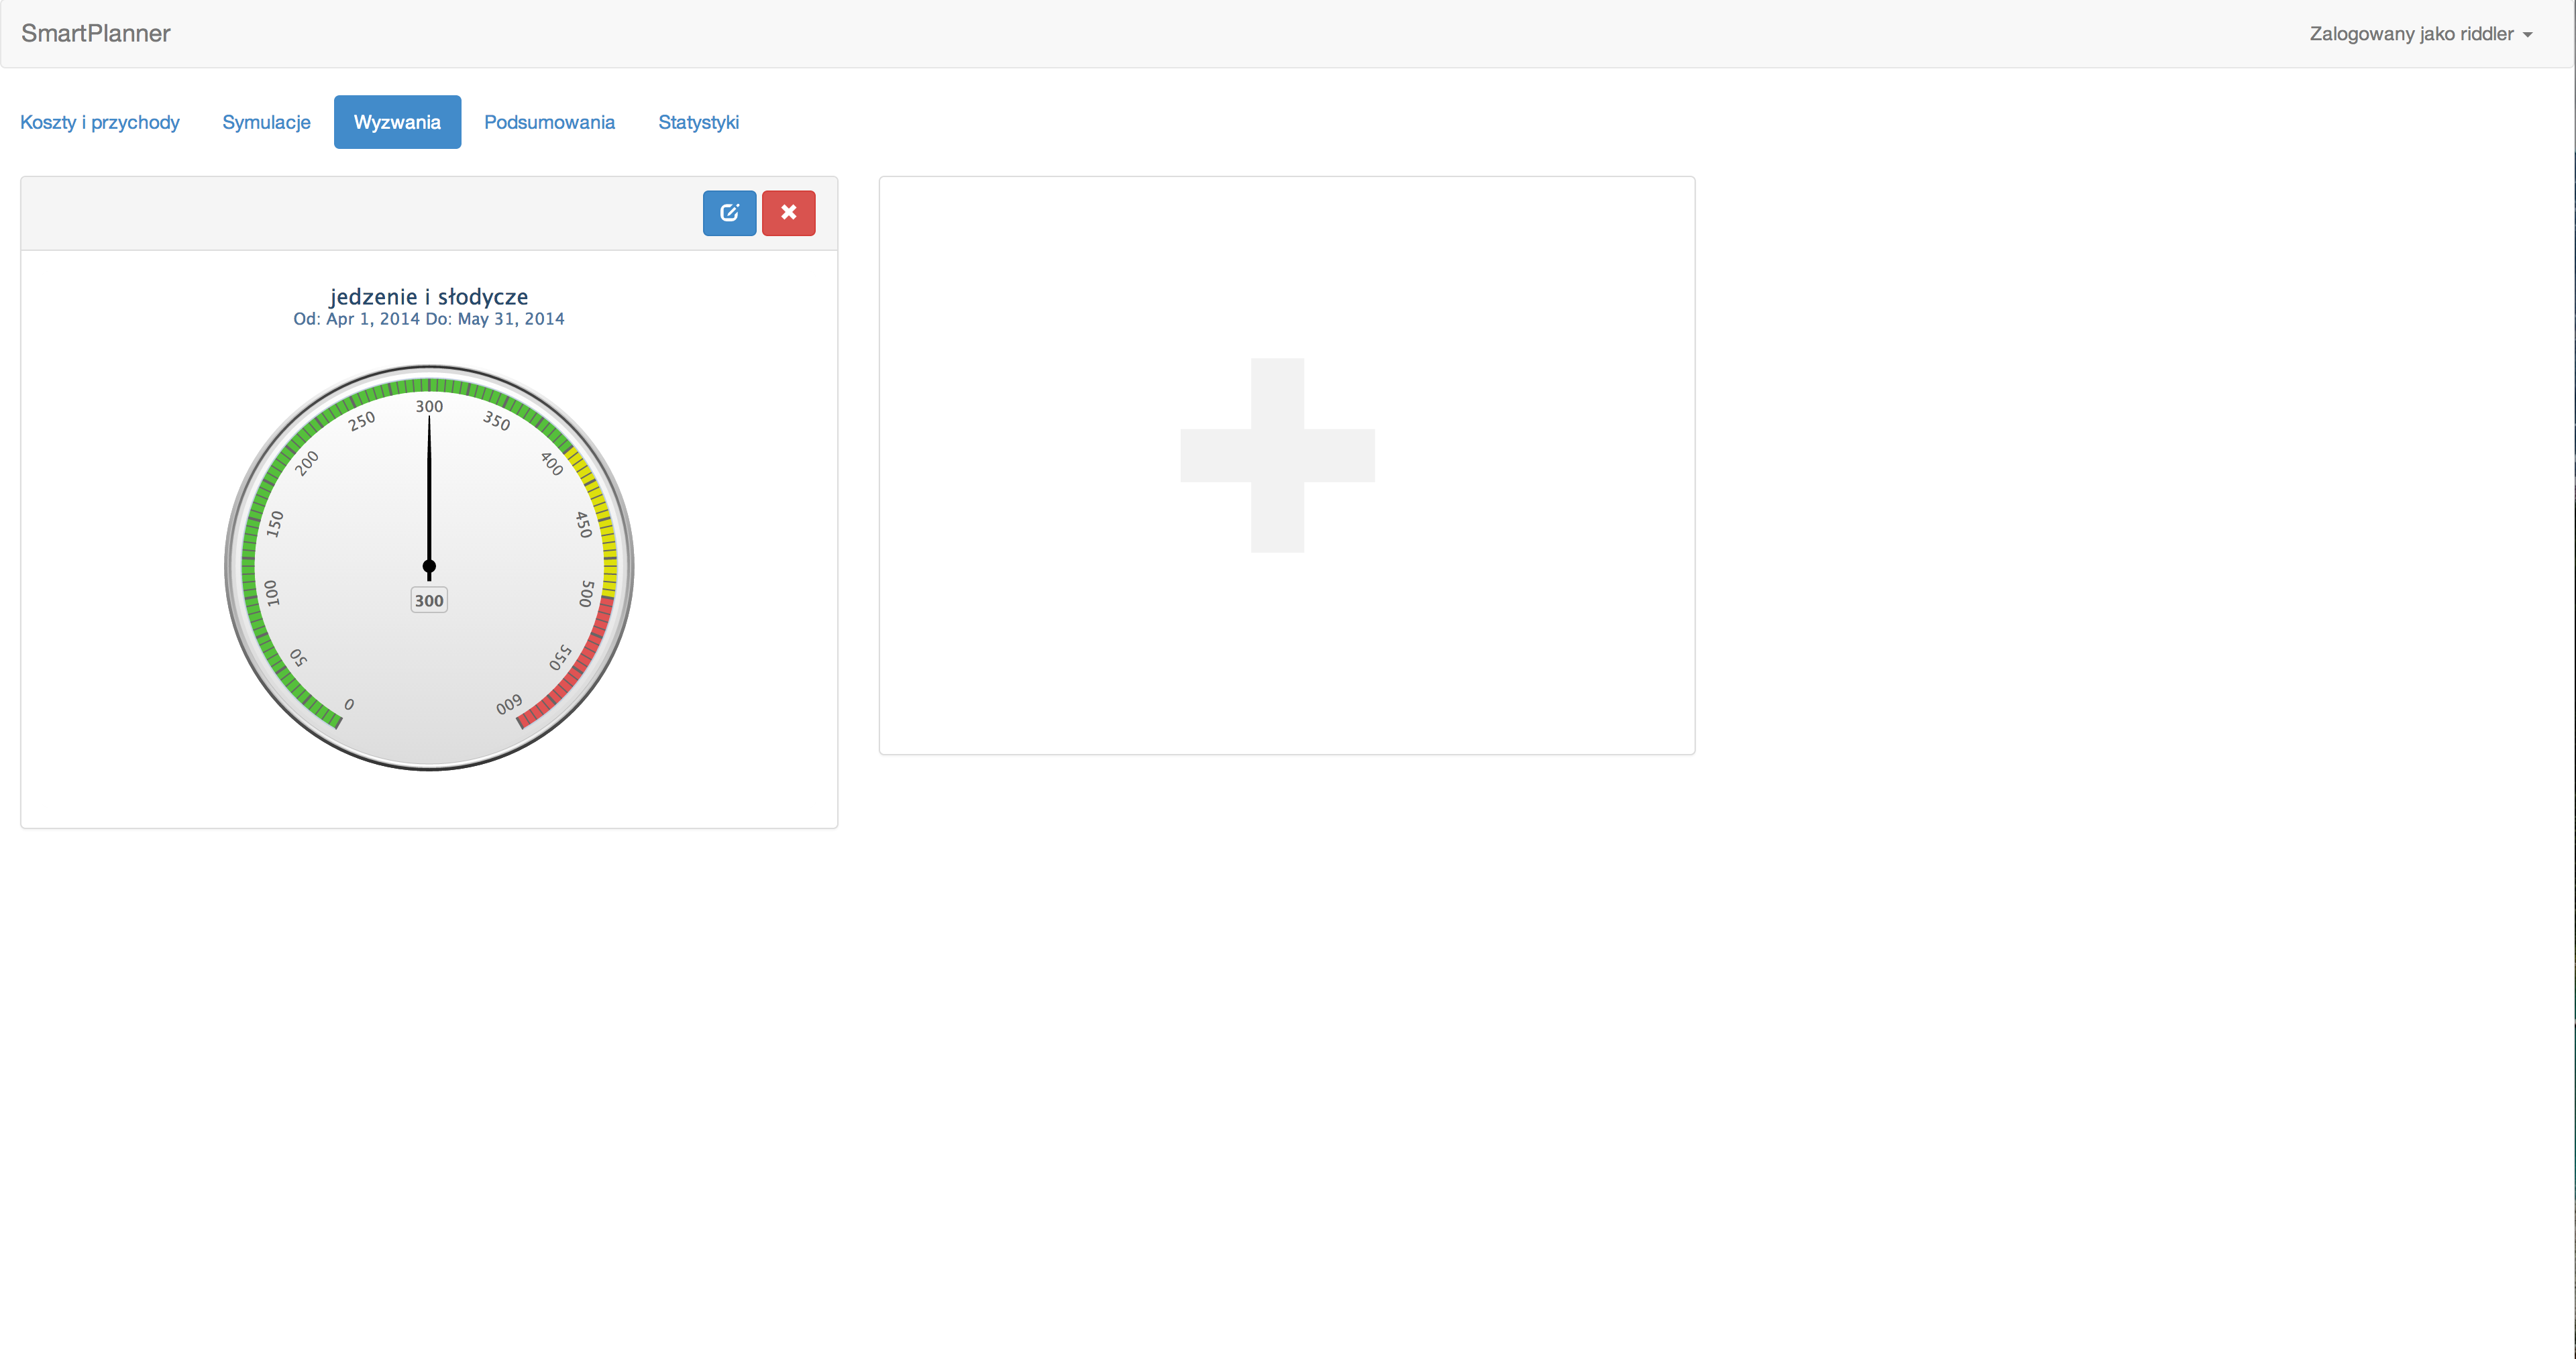
\includegraphics[scale=0.2]{images/screen_wyzwania.png}
  \caption{Lista wyzwań}
\end{figure}
\begin{figure}[H]
  \centering
  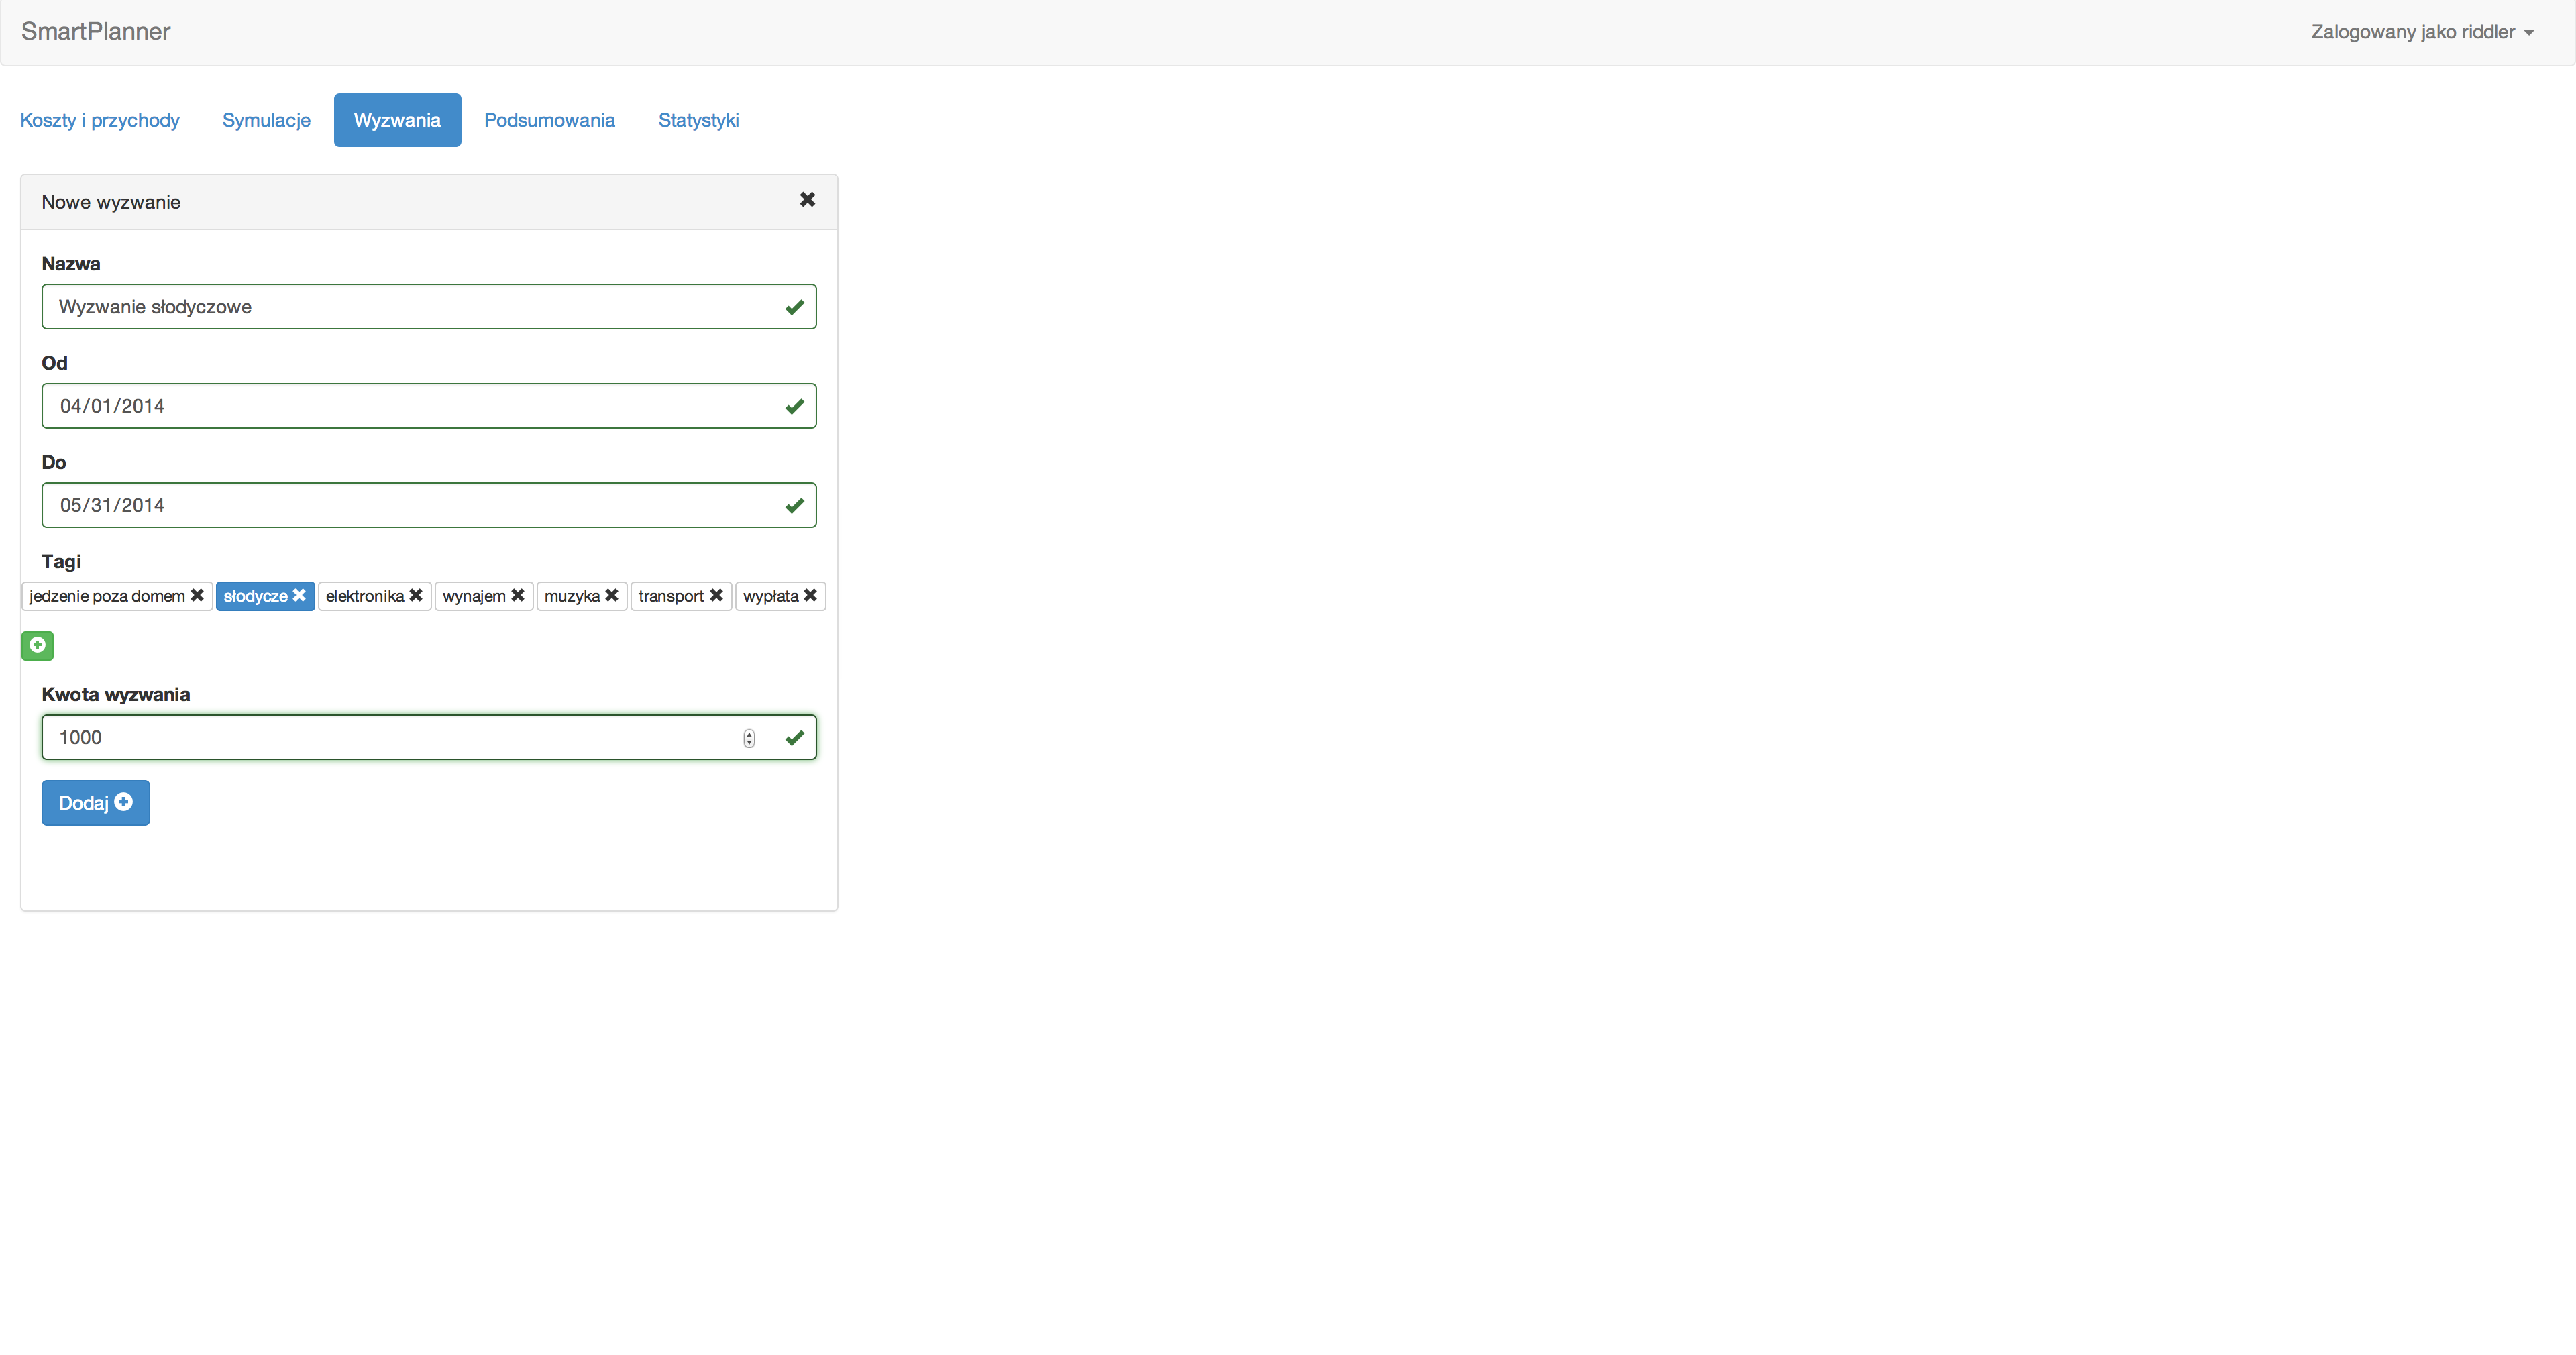
\includegraphics[scale=0.2]{images/screen_wyzwaniaDodaj.png}
  \caption{Dodawanie wyzwania}
\end{figure}
\begin{figure}[H]
  \centering
  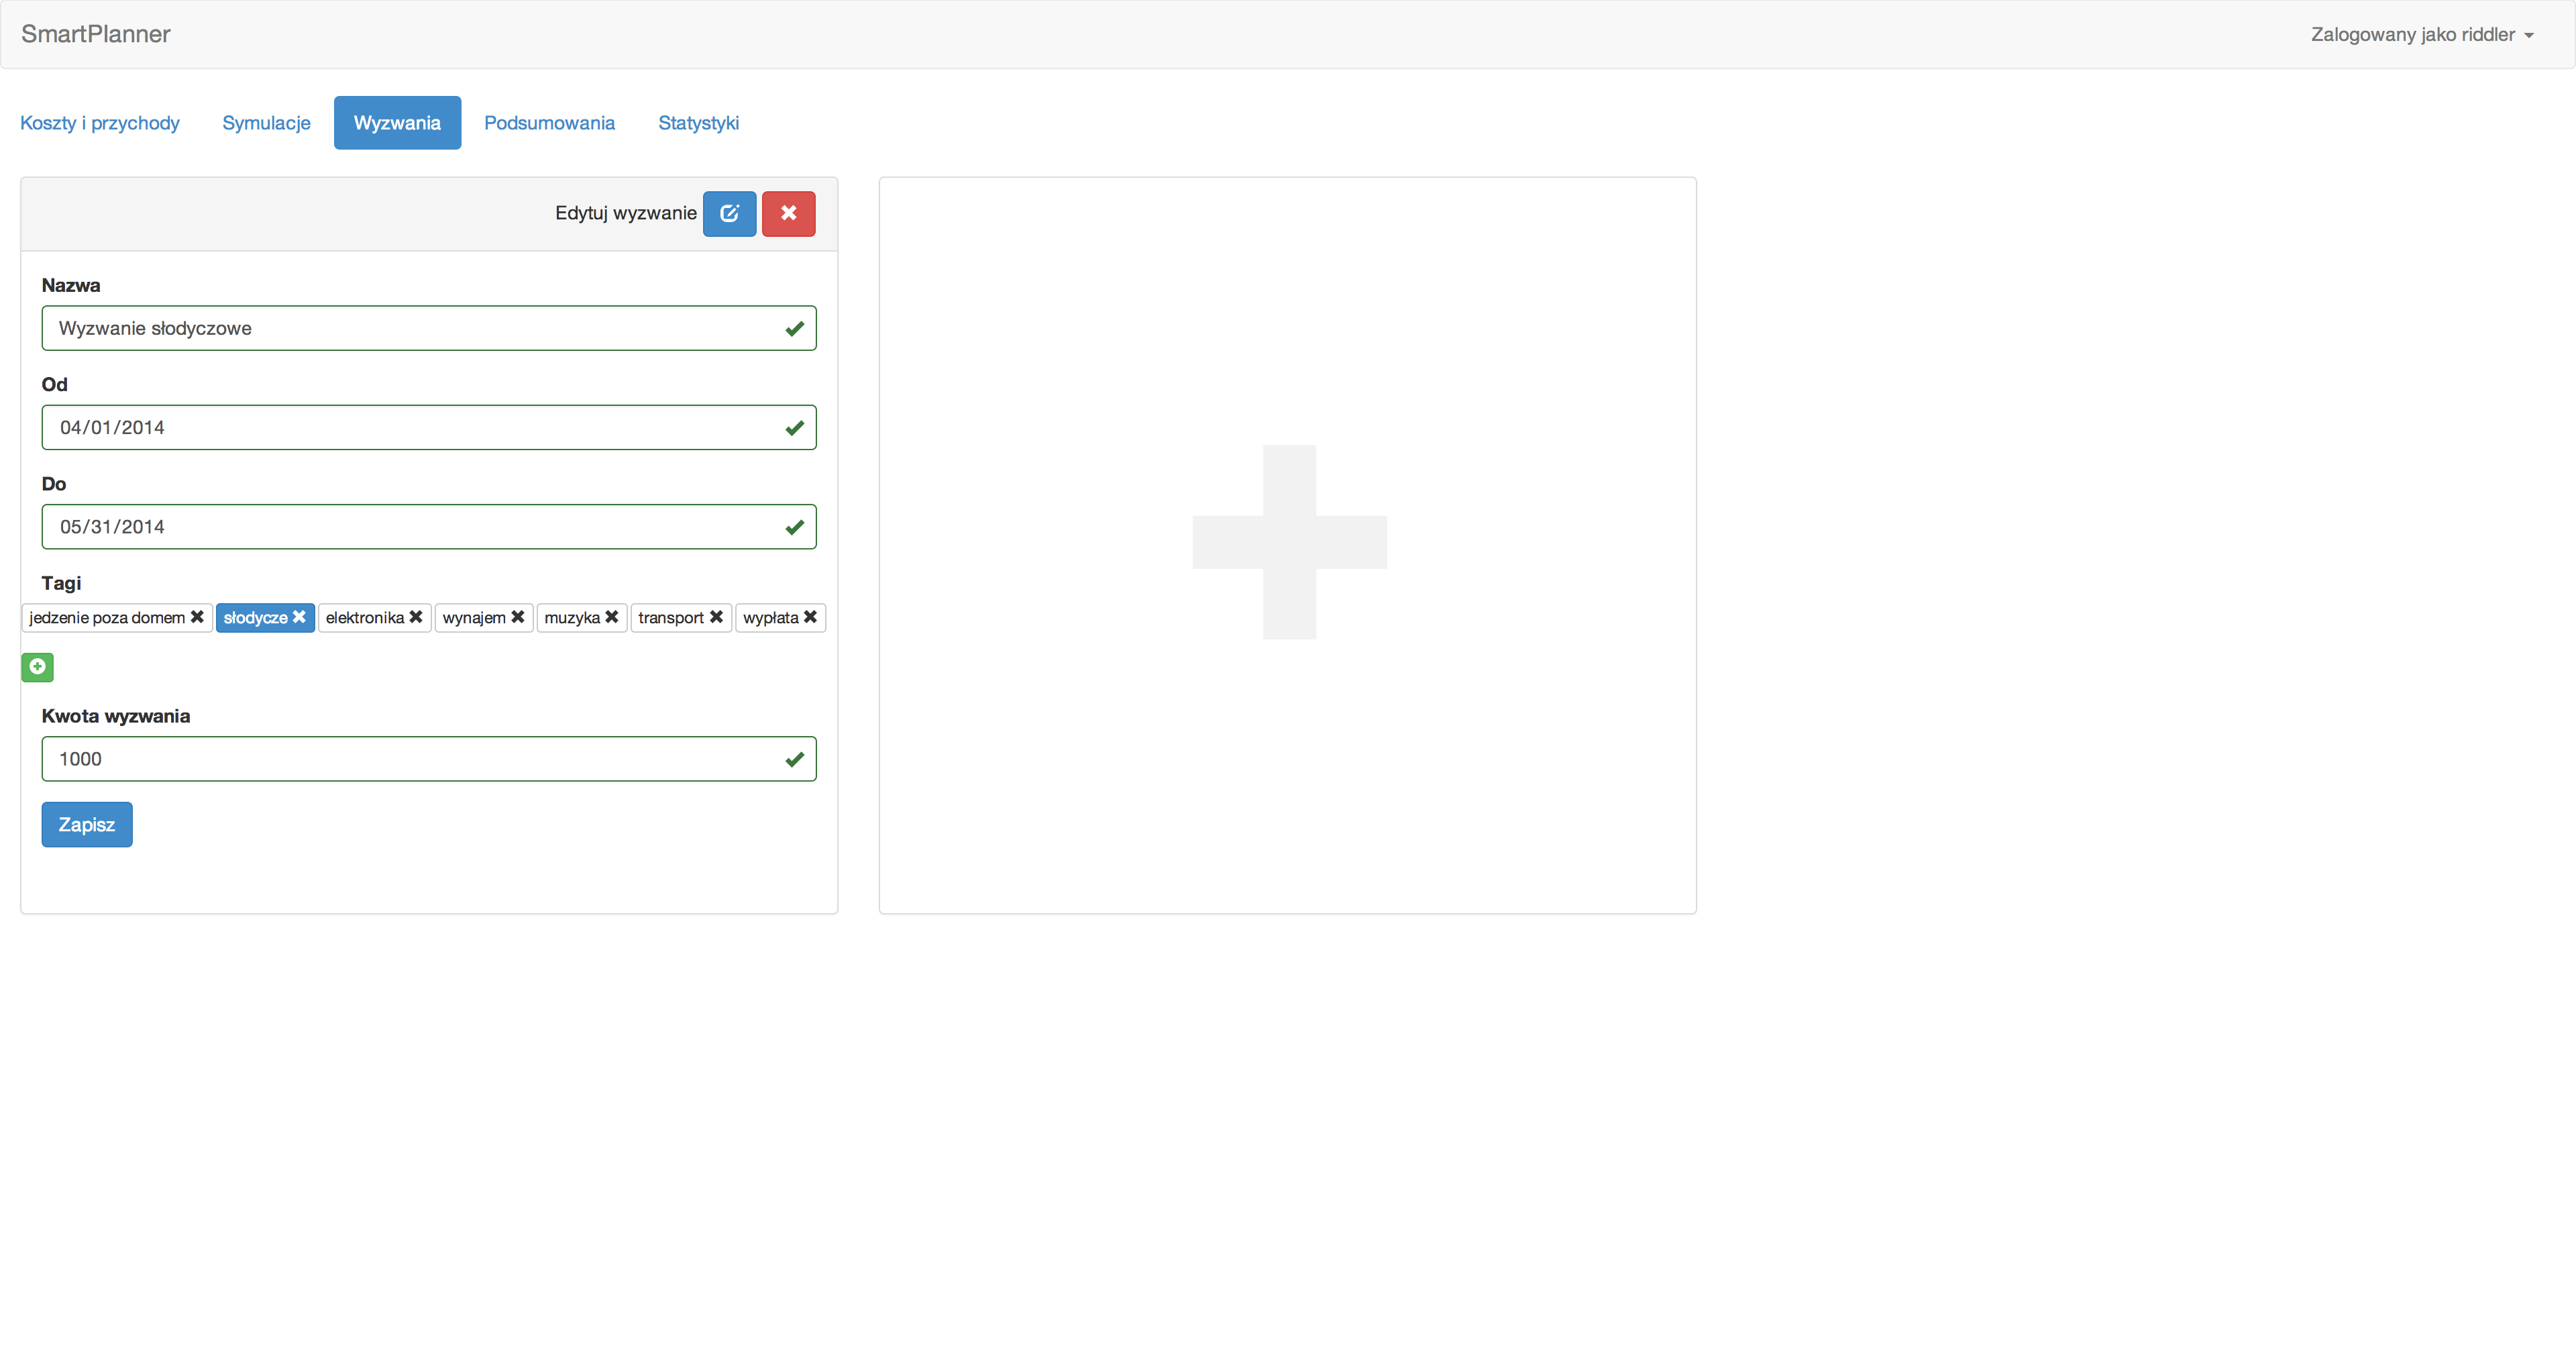
\includegraphics[scale=0.2]{images/screen_wyzwaniaEdycja.png}
  \caption{Edycja wyzwania}
\end{figure}
\begin{figure}[H]
  \centering
  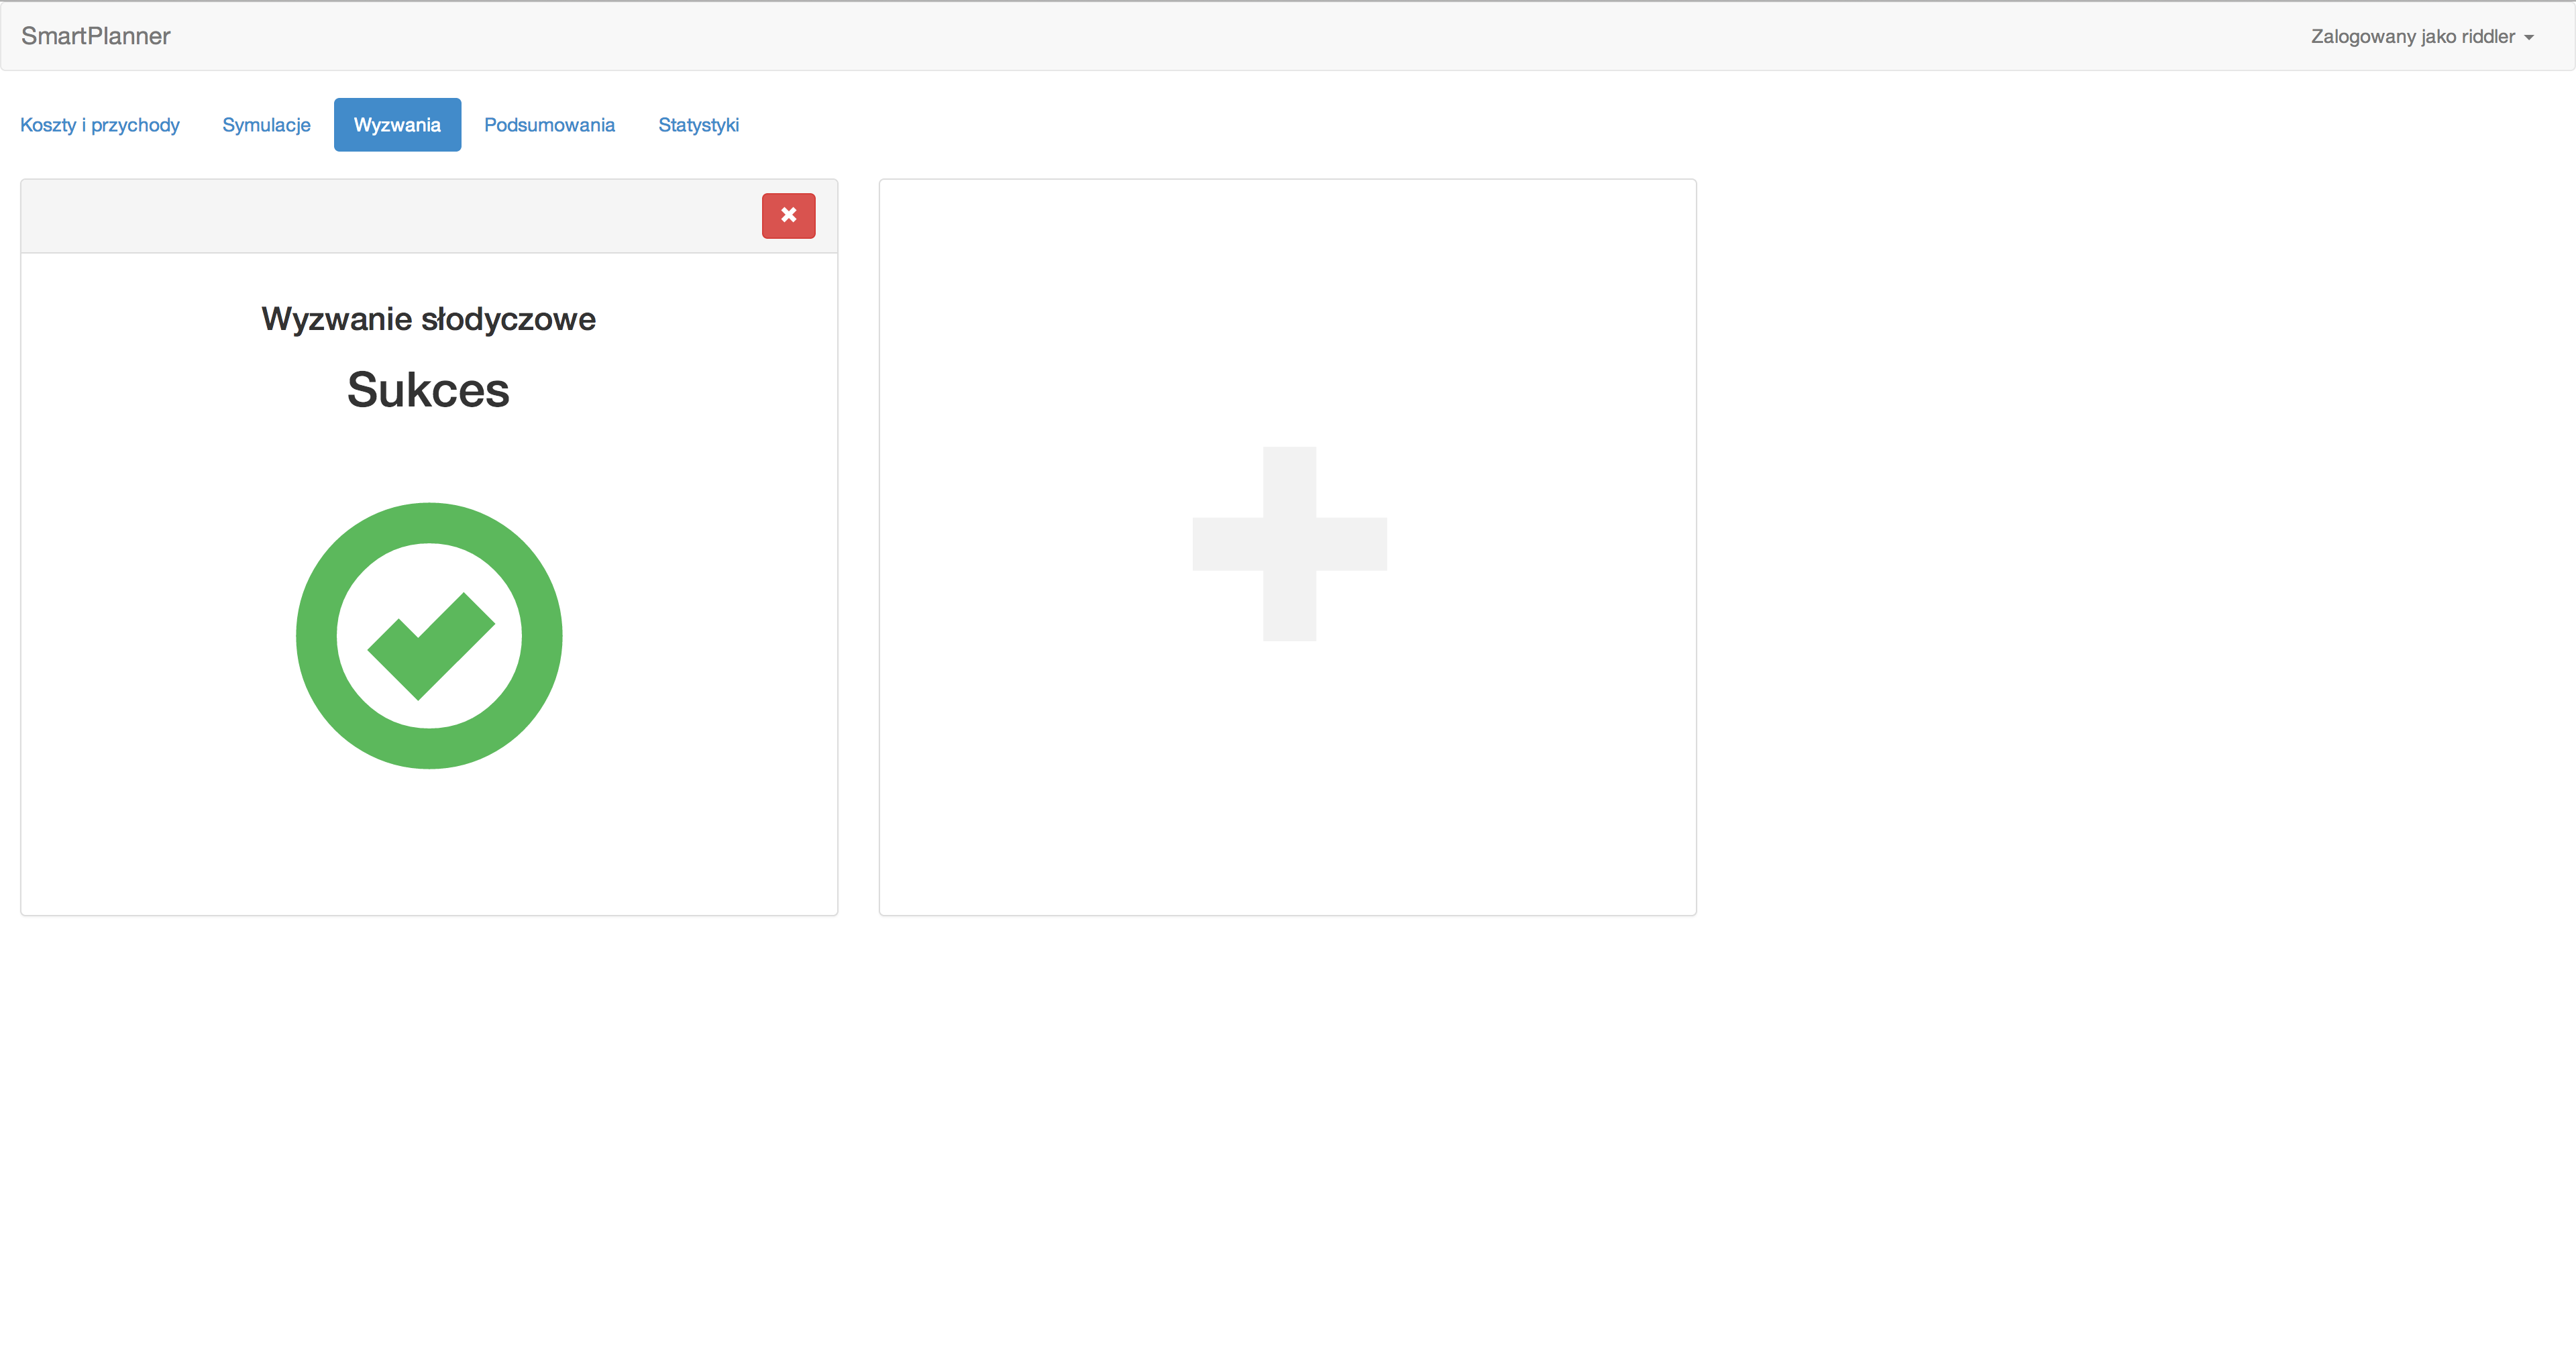
\includegraphics[scale=0.2]{images/screen_wyzwaniaSukces.png}
  \caption{Sukces w wyzwaniu}
\end{figure}
\begin{figure}[H]
  \centering
  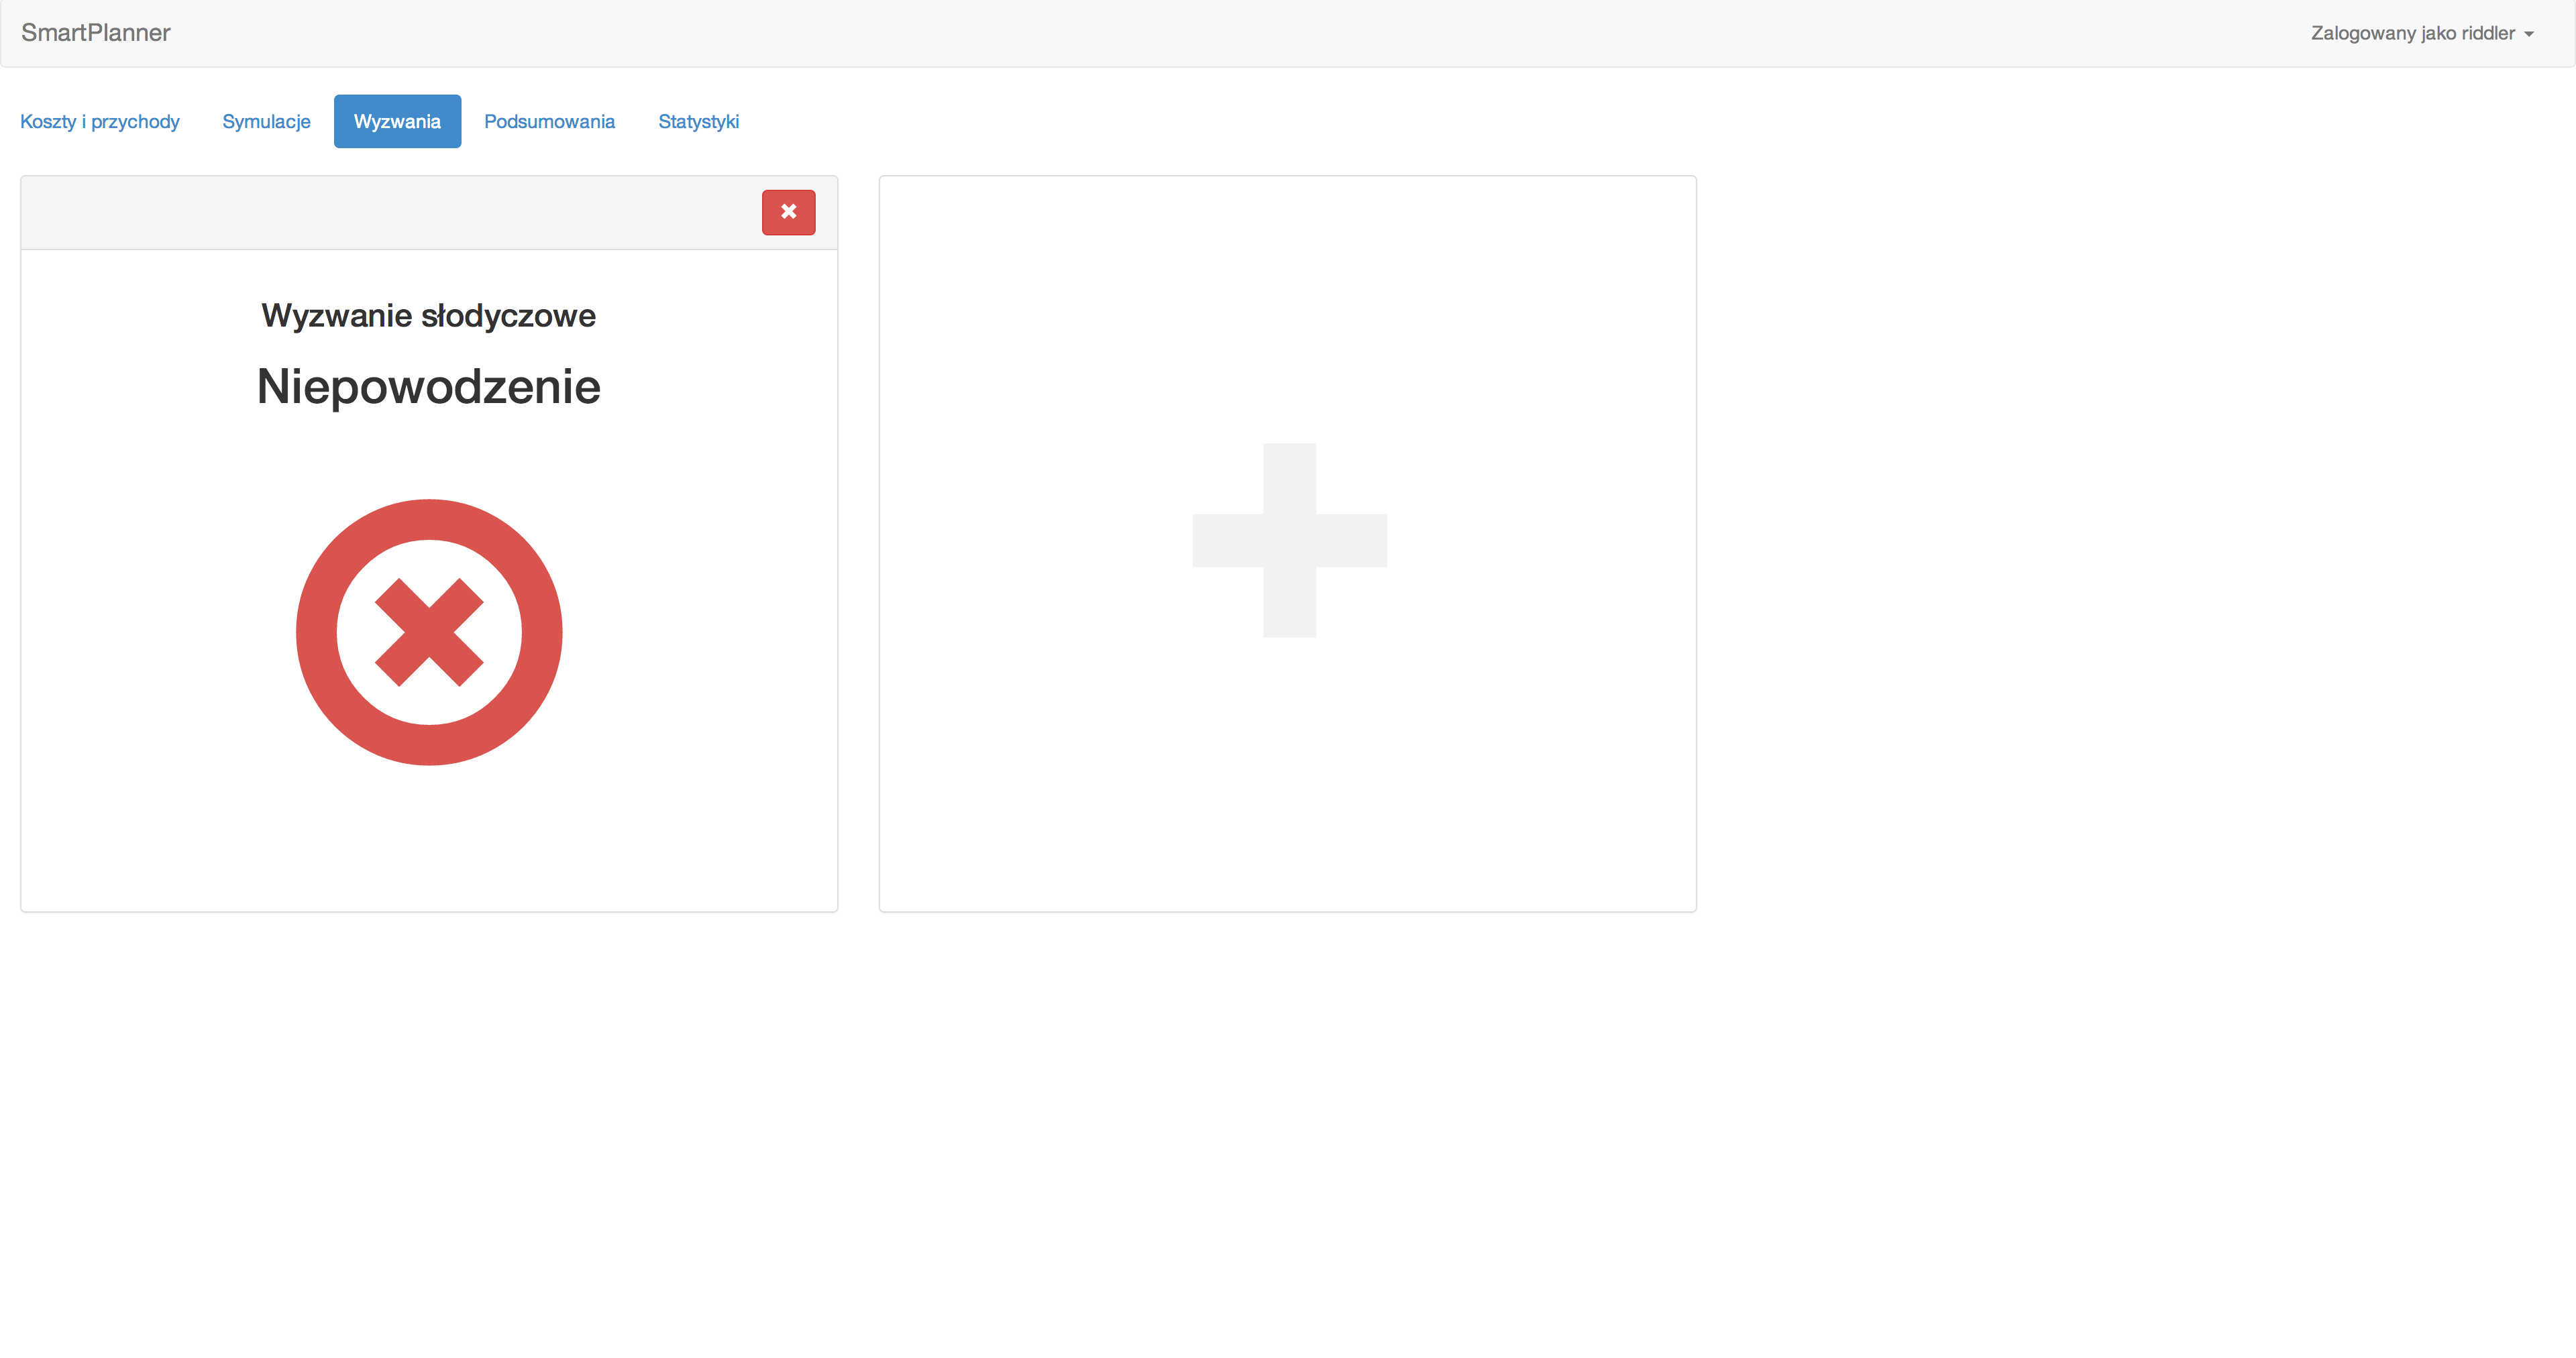
\includegraphics[scale=0.2]{images/screen_wyzwaniaNiepowodzenie.png}
  \caption{Niepowodzenie w wyzwaniu}
\end{figure}
Na ekranie pokazane są statystyki predefiniowane przez twórcę aplikacji i nie można ich zmienić. Po naciśnięciu jakiegoś elementu na wykresie zostajemy przeniesieni na widok z rysunku nr ~\ref{screen:listExpense} \\ z wyfiltrowanymi wydatkami.
\begin{figure}[H]
  \centering
  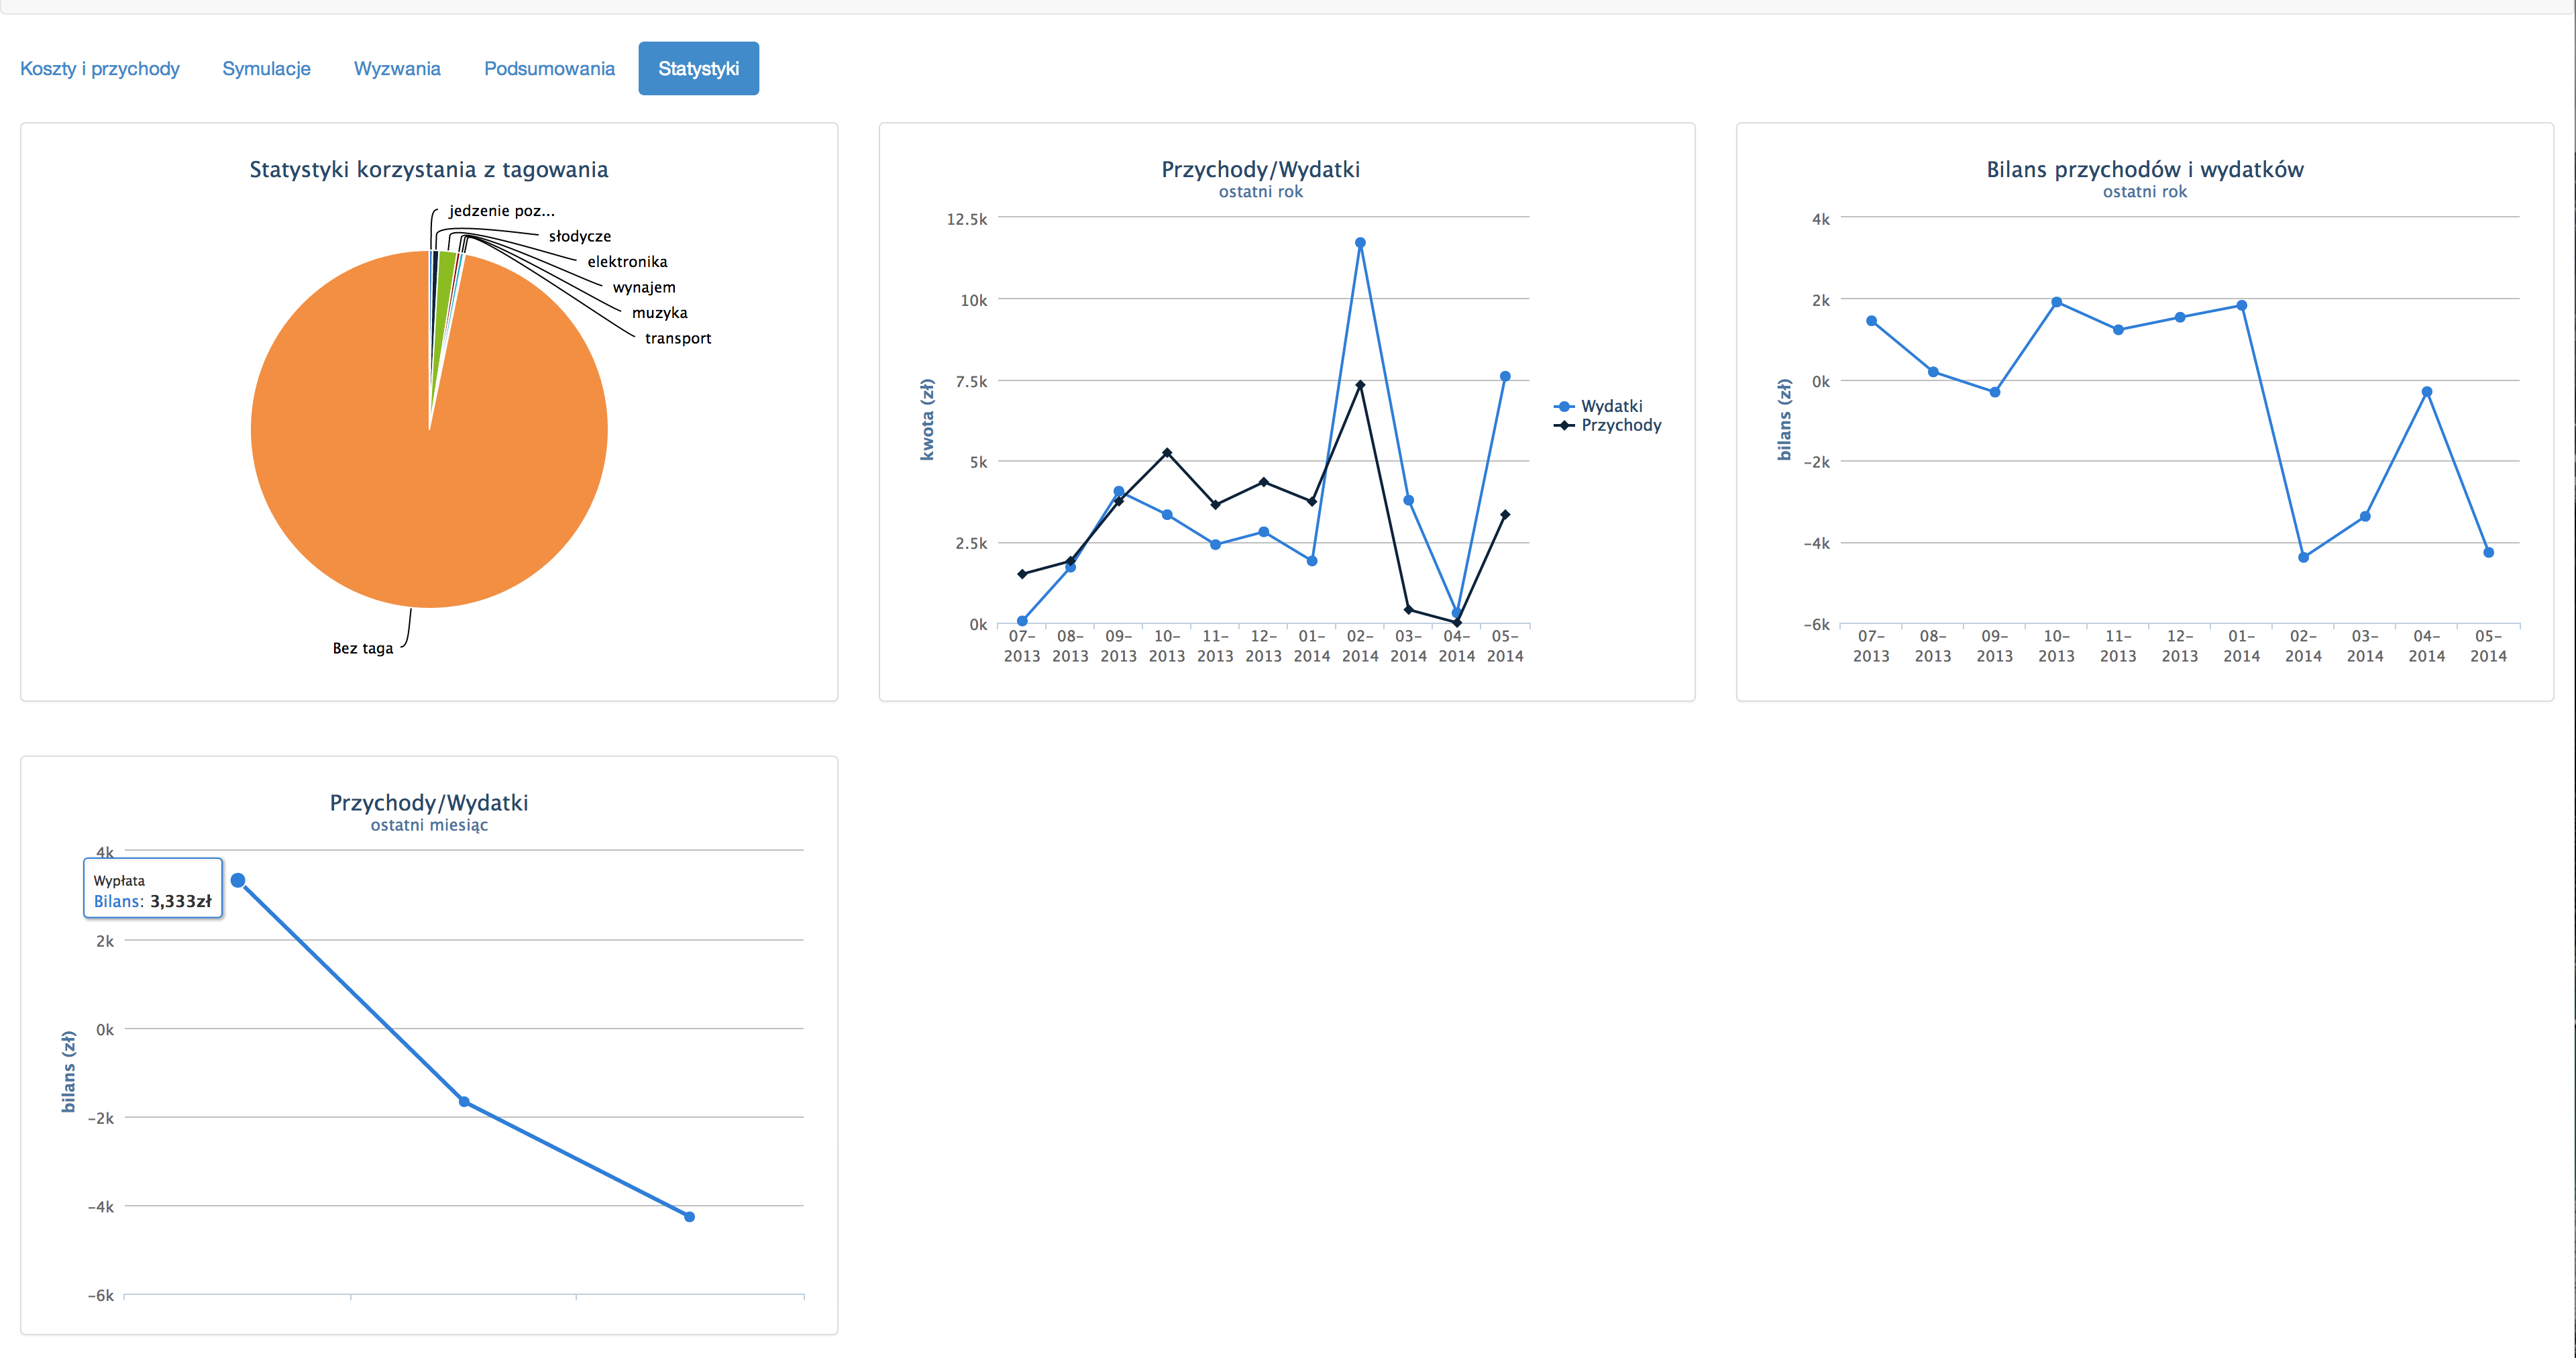
\includegraphics[scale=0.2]{images/screen_statystyki.png}
  \caption{Statystyki}
\end{figure}
\section{Instalacja i wdrożenie}
Aby wdrożyć aplikację potrzebujemy następujących składników:
\begin{itemize}
  \item Microsoft Windows 2012 Server/7/8 lub wyższe
  \item .NET Framework 4.5
  \item Microsoft SQL Server 2012 lub wyższe
  \item Microsoft IIS Server 7
\end{itemize}
Przedstawiona poniżej instalacja została wykonana na systemie Windows 8.1

\par Pierwszym krokiem jest instalajca serwera IIS. Aby to zrobić trzeba przejść do \verb|Control Panel|, a następnie do \verb|Programs and features| pokazane na obrazku nr ~\ref{install:programs}.
\par Tutaj należy kliknąć \verb|Turn Windows features on or off|.
\begin{figure}[H]
  \centering
  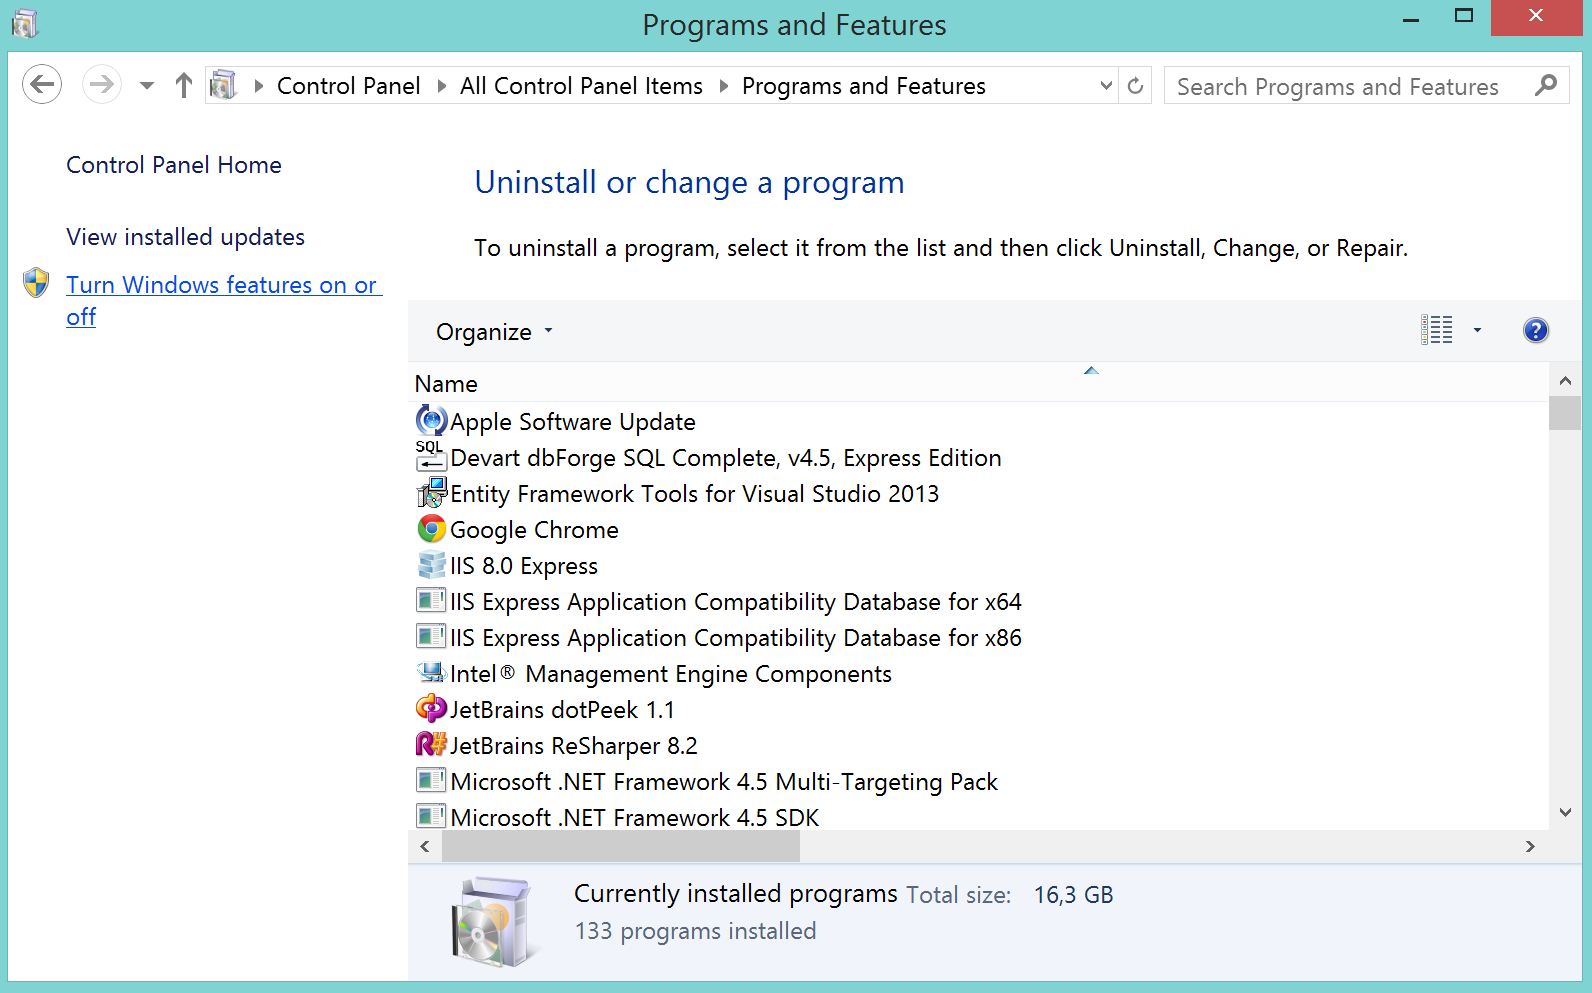
\includegraphics[scale=0.35]{images/install1.png}
  \caption{Programs and features}
  \label{install:programs}
\end{figure}
\par Zaznaczyć \verb|Internet Information Services|, a następnie kliknąć ok, po naciśnięciu którego nastąpi instalacja IIS.
\begin{figure}[H]
  \centering
  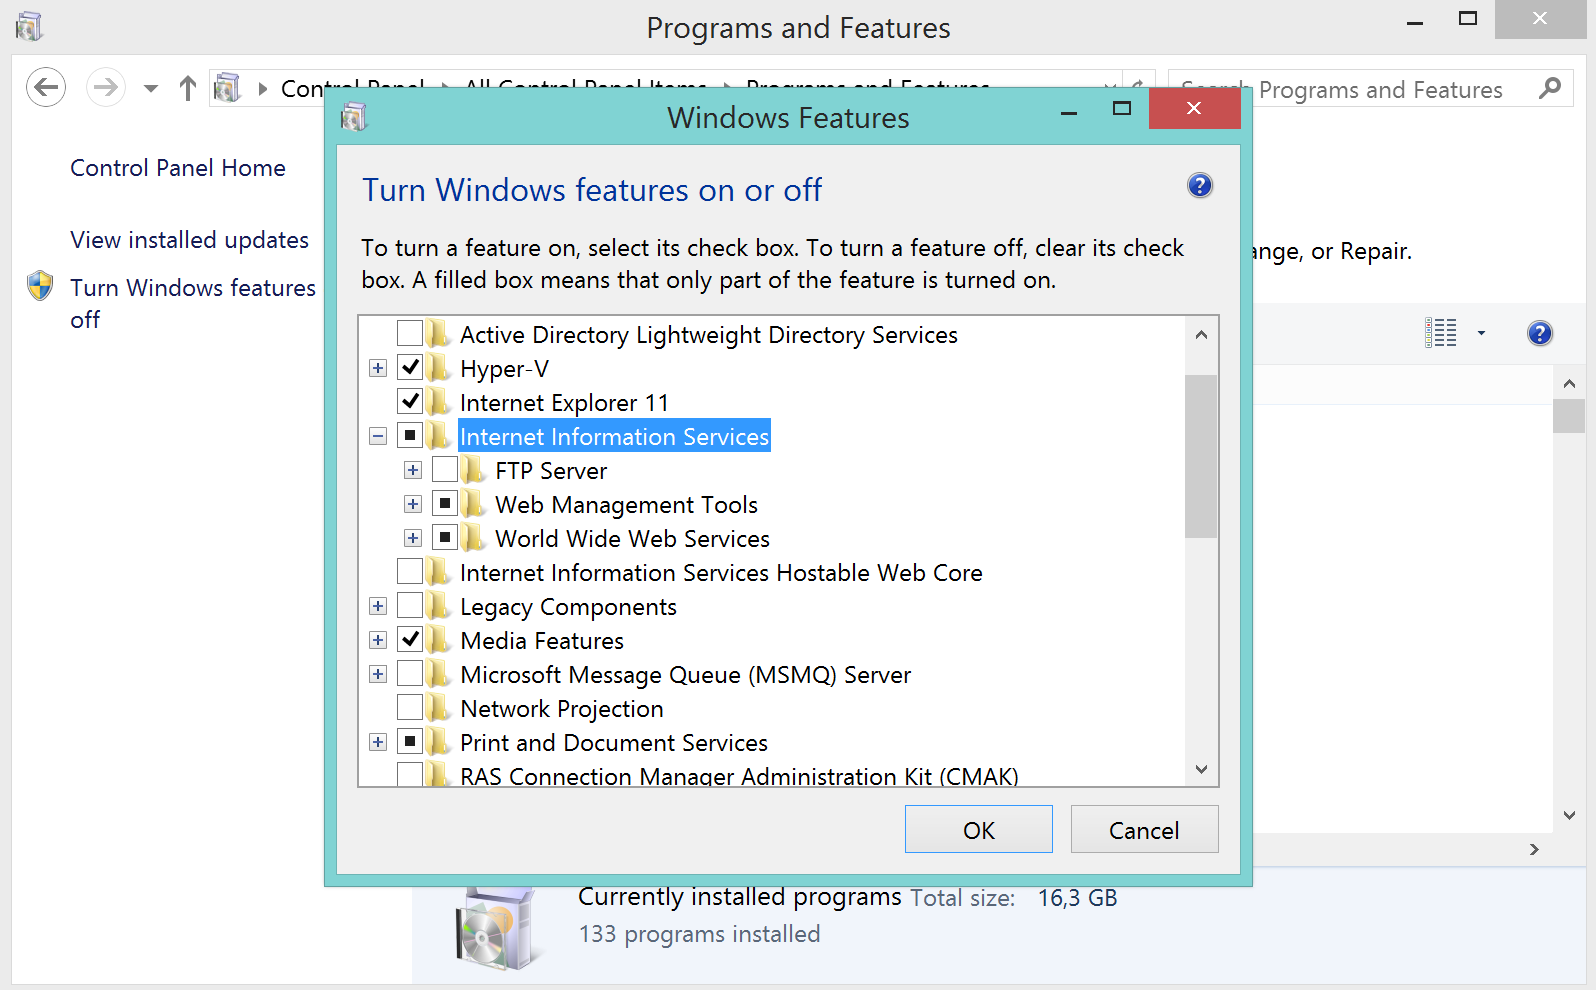
\includegraphics[scale=0.35]{images/install2.png}
  \caption{Turn Windows features on or off}
\end{figure}
\par Ten ekran prezentuje powodzenie instalacji IIS.
\begin{figure}[H]
  \centering
  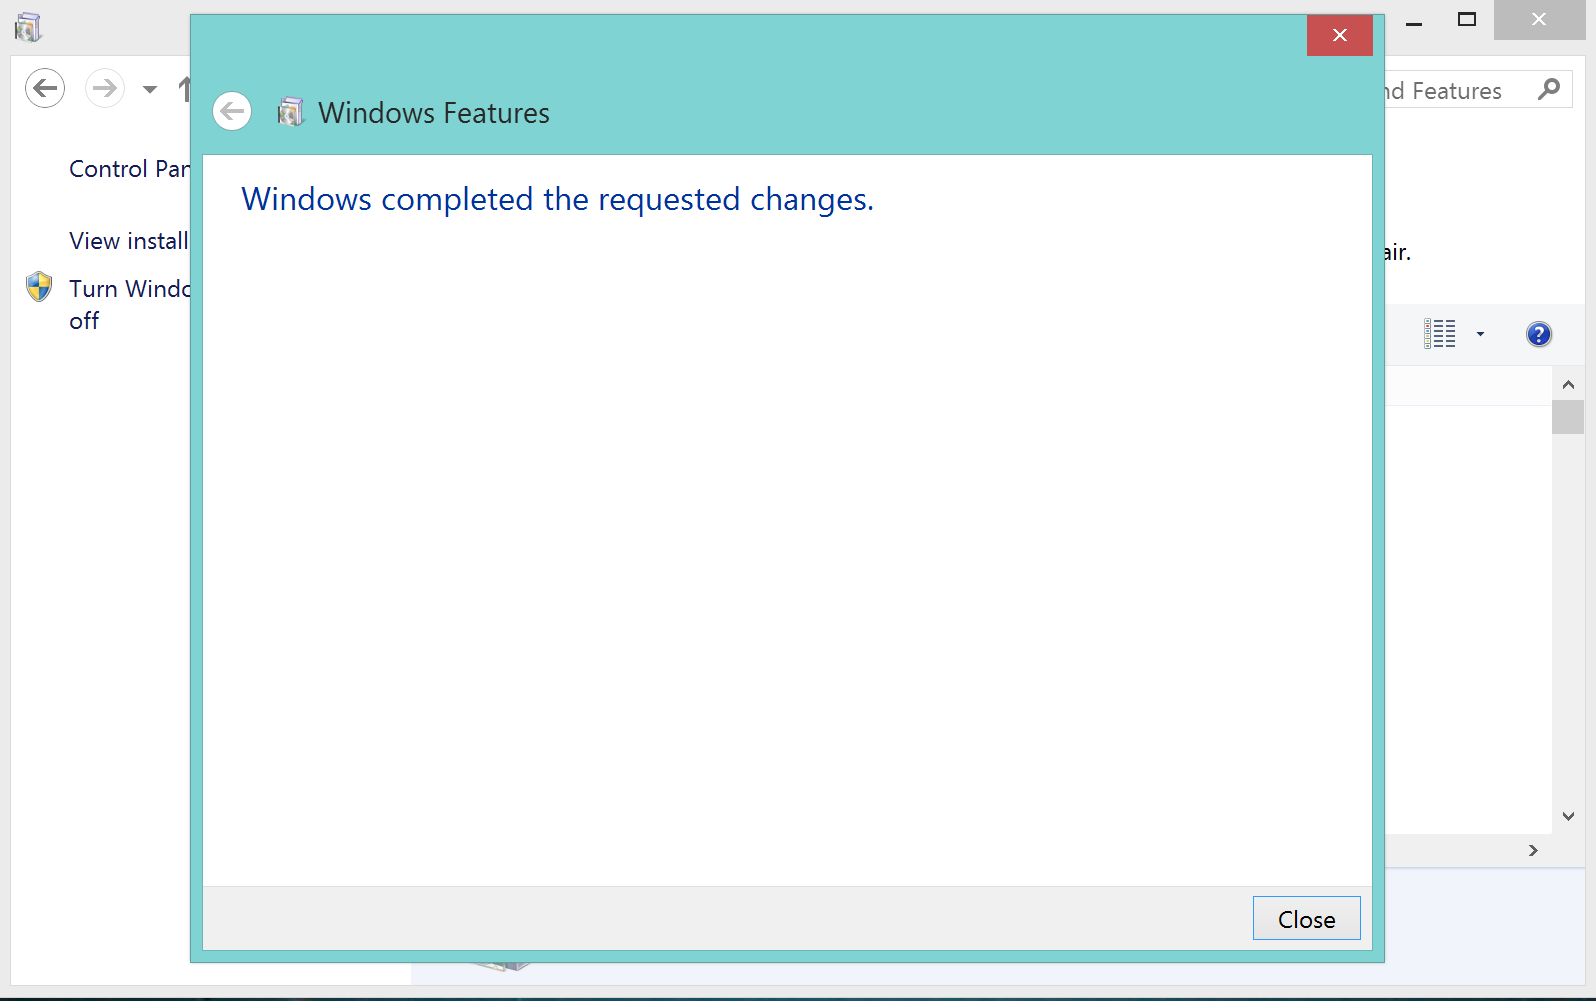
\includegraphics[scale=0.35]{images/install3.png}
  \caption{Powodzenie installacji IIS}
\end{figure}
\par Kolejnym krokiem jest skonfigurowanie IIS pod aplikację. Aby to wykonać trzeba przejść do \textbf{Control Panel} > \textbf{Administrative Tools} > \textbf{Internet Information Services (IIS) Manager}
\begin{figure}[H]
  \centering
  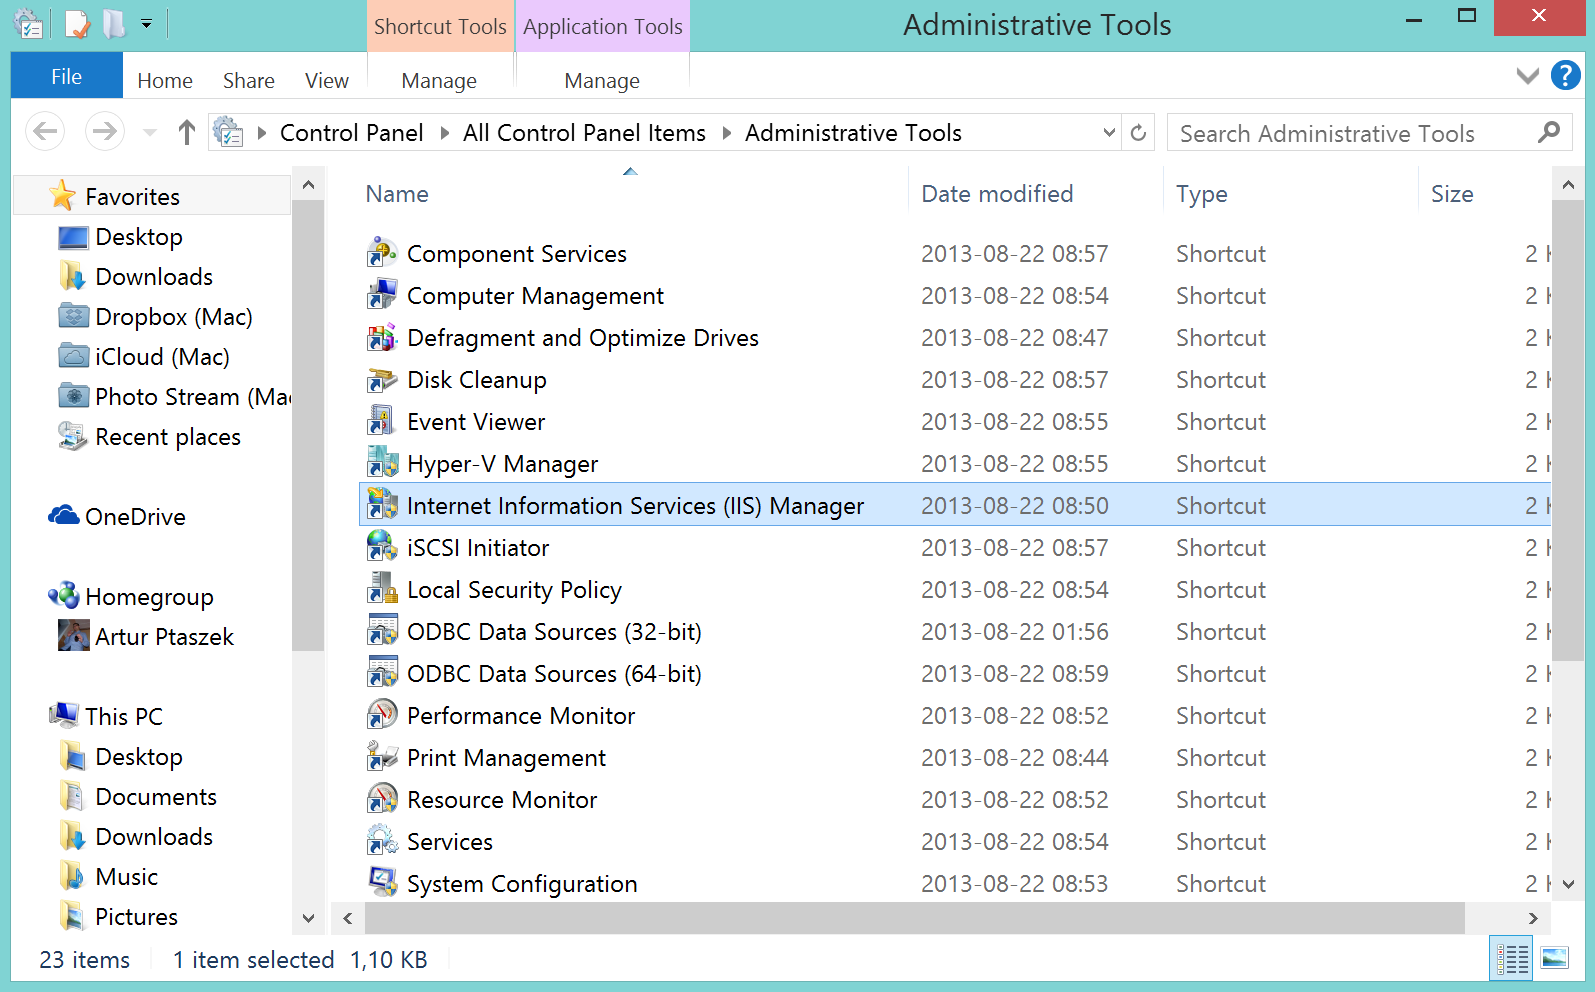
\includegraphics[scale=0.35]{images/install4.png}
  \caption{Internet Information Services (IIS) Manager}
\end{figure}
\par W lewej kolumnie wybieramy \verb|Application Pools| i w prawej \verb|Add Application Pool...|
\begin{figure}[H]
  \centering
  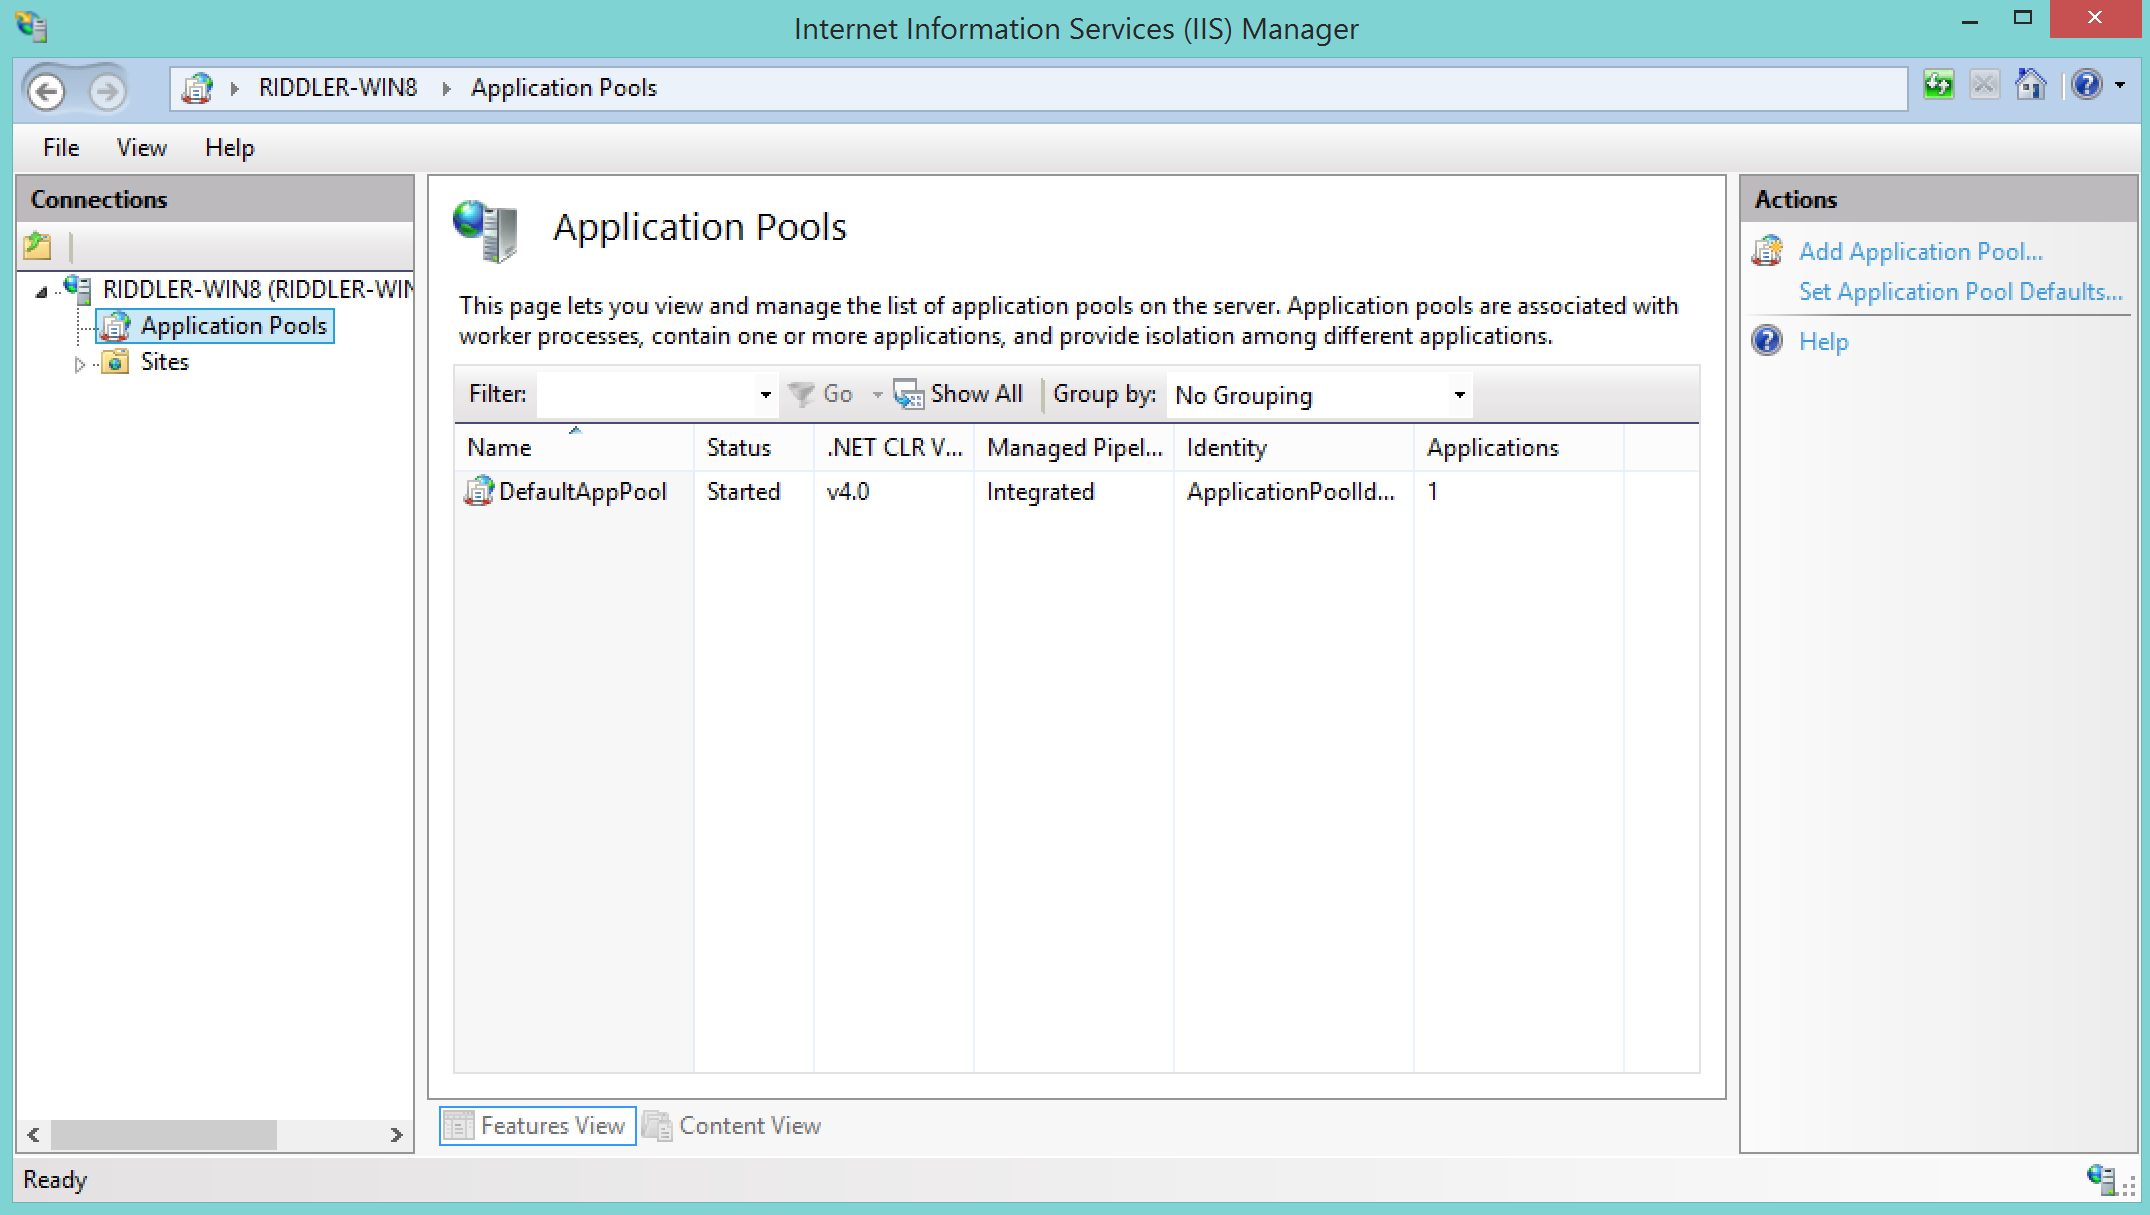
\includegraphics[scale=0.35]{images/install5.png}
  \caption{Internet Information Services (IIS) Manager}
\end{figure}
\par Należy wypełnić dane tak jak w okienku poniżej i kliknąć OK.
\begin{figure}[H]
  \centering
  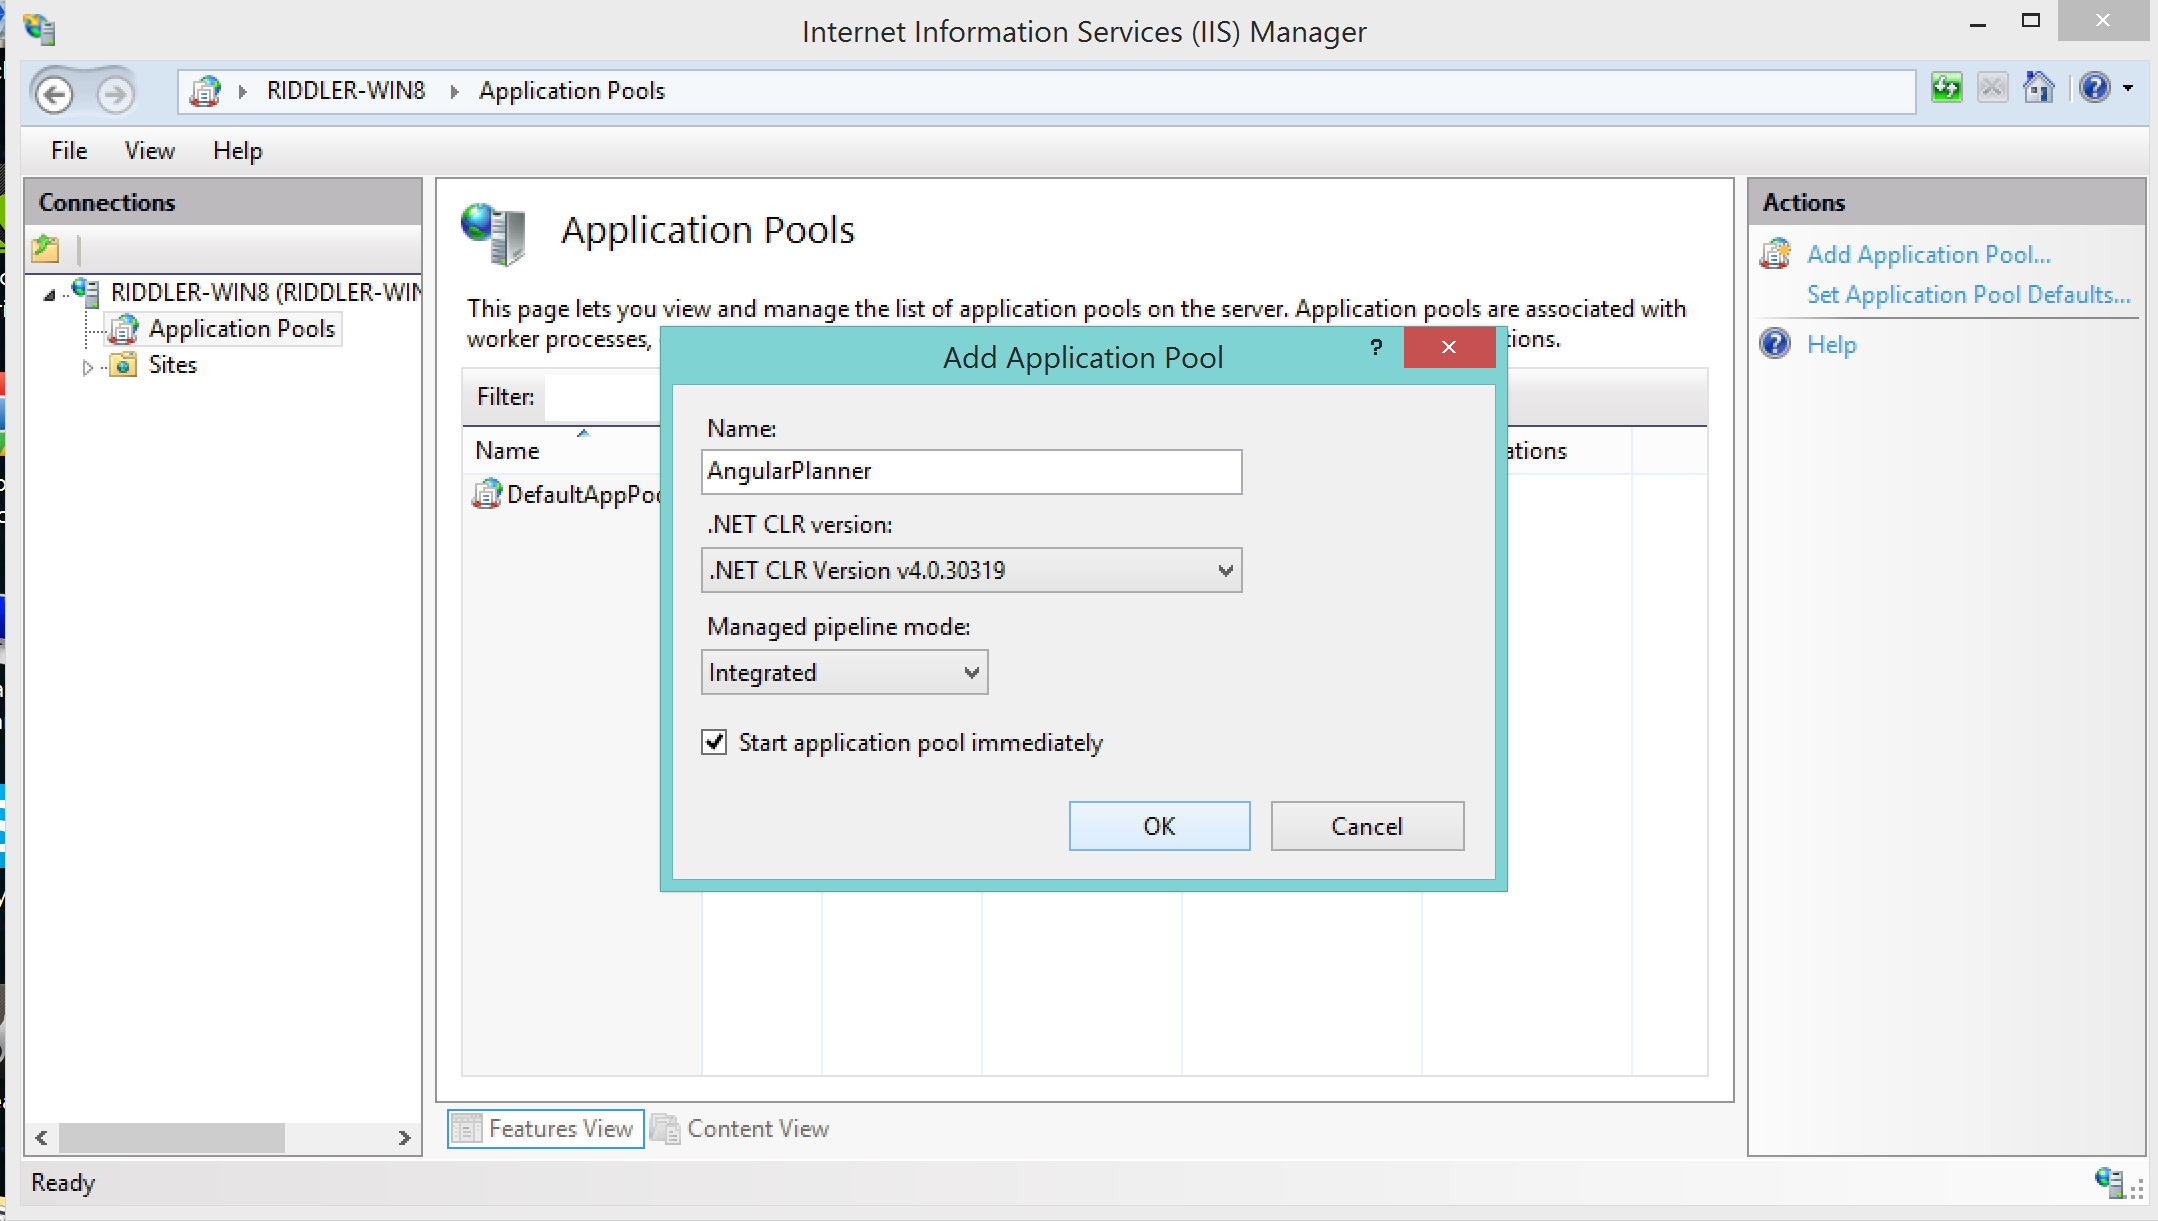
\includegraphics[scale=0.35]{images/install6.png}
  \caption{Dodawanie nowej puli}
\end{figure}
\par Z lewej kolumny należy wybrać \verb|Sites| i w prawej kliknąć \verb|Add Website|.
\begin{figure}[H]
  \centering
  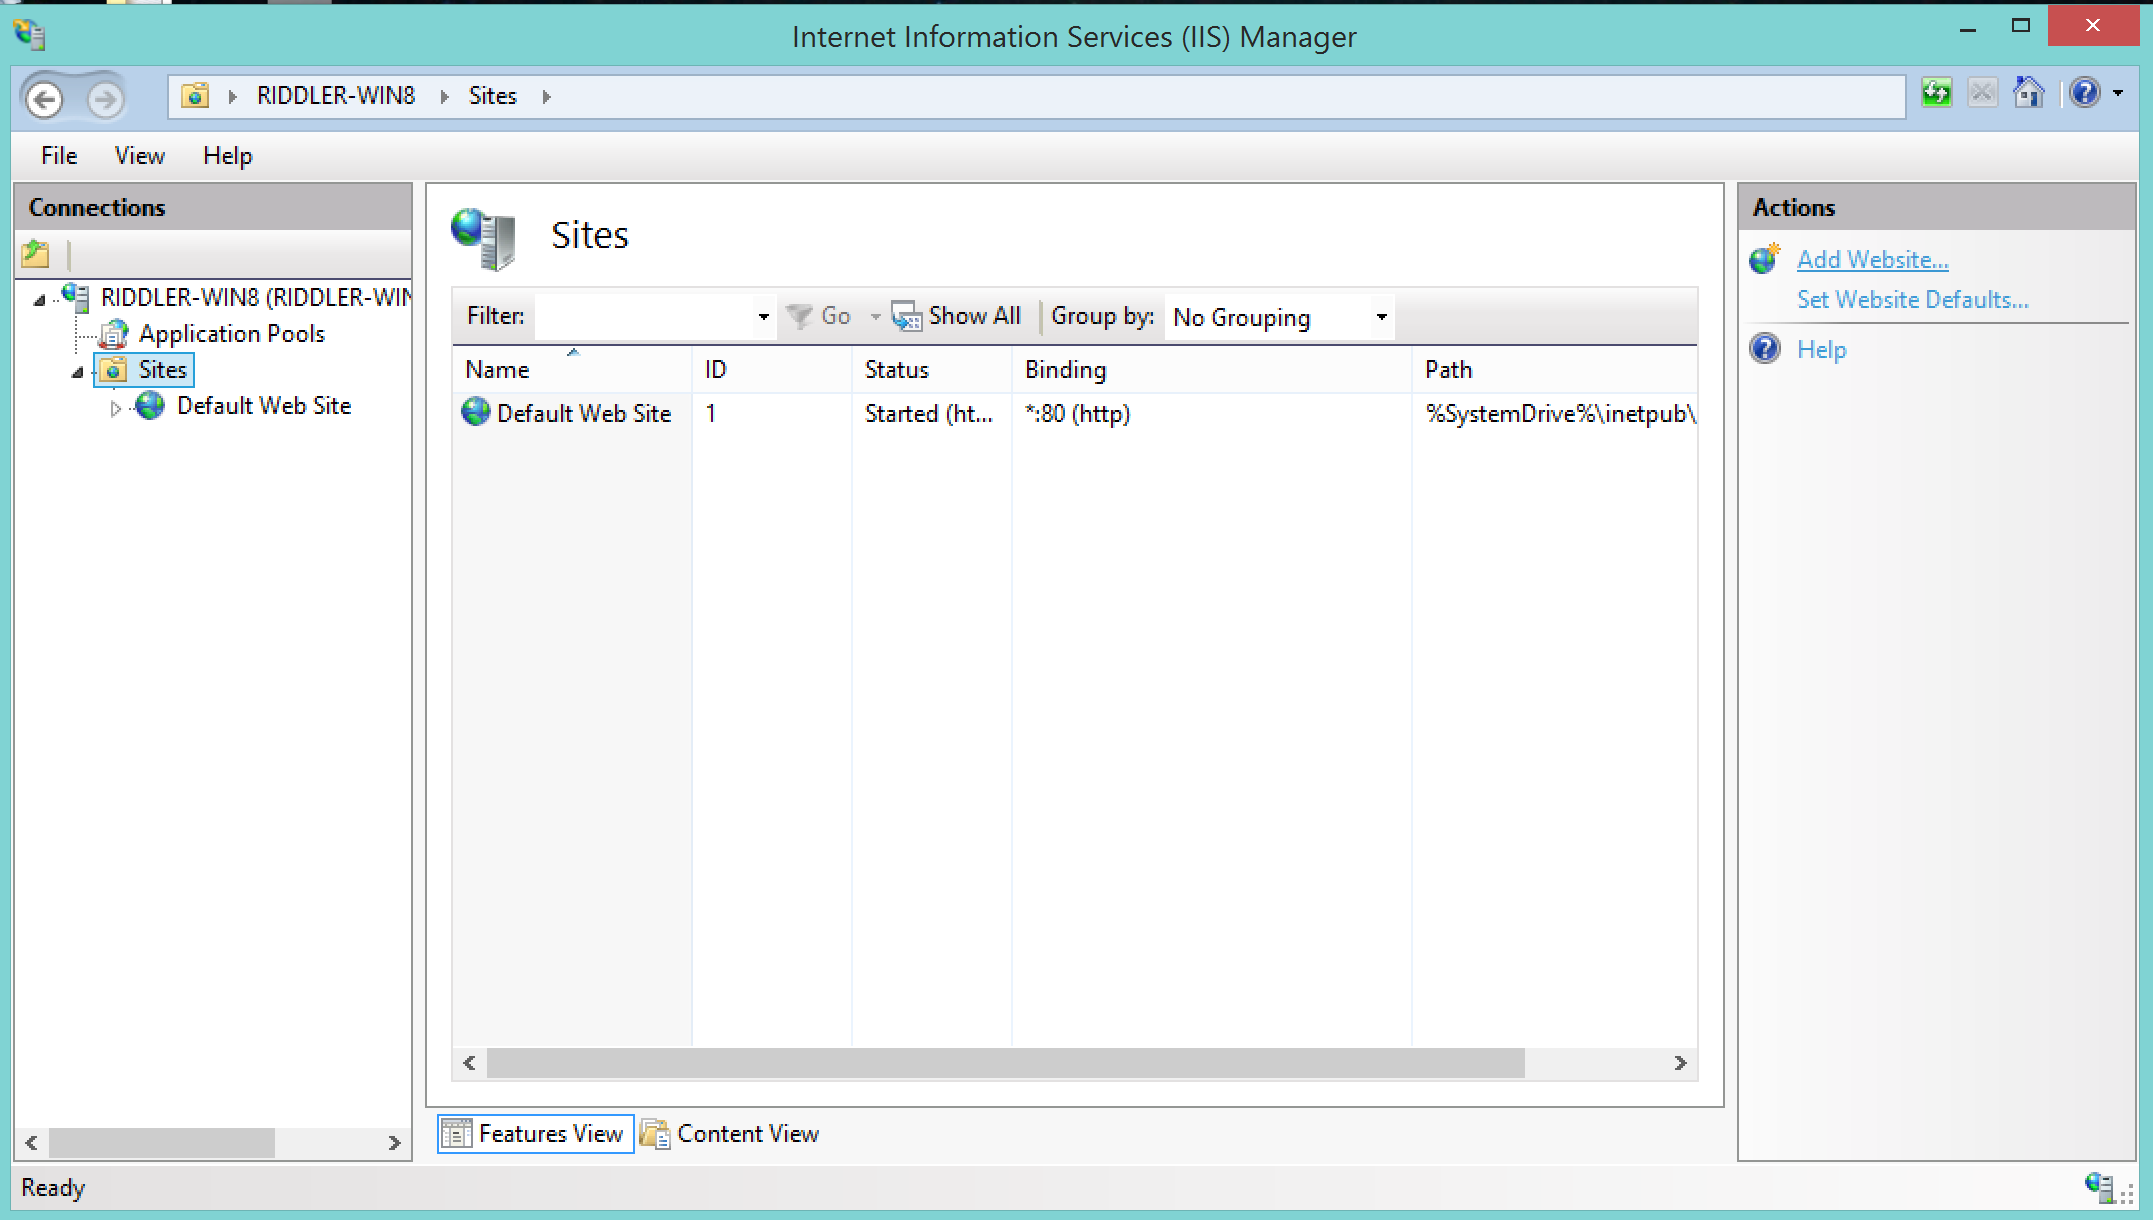
\includegraphics[scale=0.35]{images/install7.png}
  \caption{Internet Information Services (IIS) Manager}
\end{figure}
\begin{figure}[H]
  \centering
  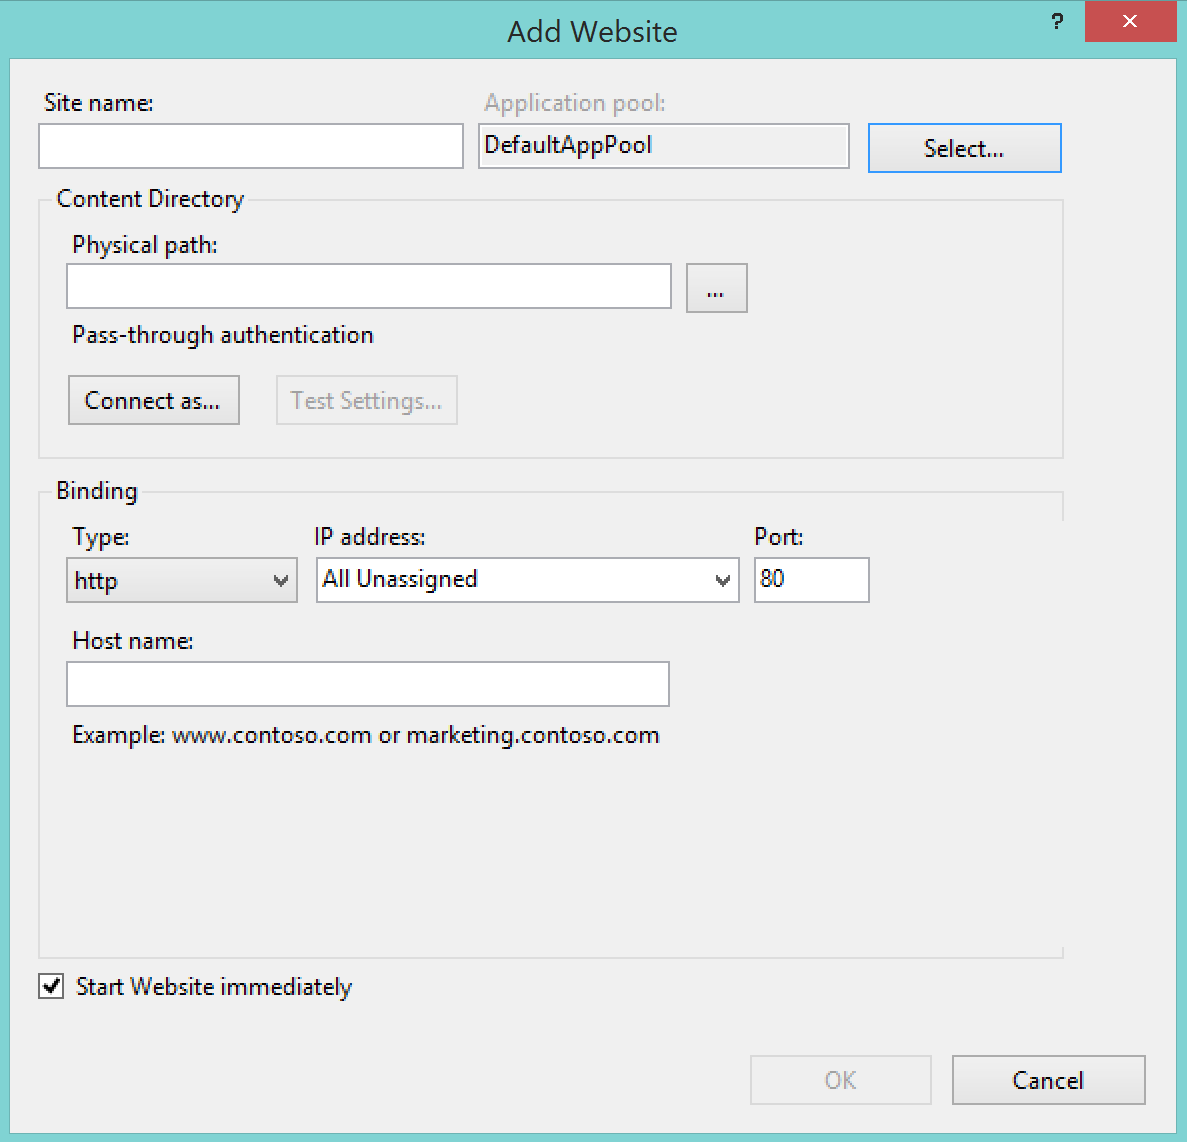
\includegraphics[scale=0.35]{images/install8.png}
  \caption{Dodawanie strony}
\end{figure}
\par Należy kliknąć przycisk \verb|Select...| i wybrać pule \verb|AngularPlanner|.
\begin{figure}[H]
  \centering
  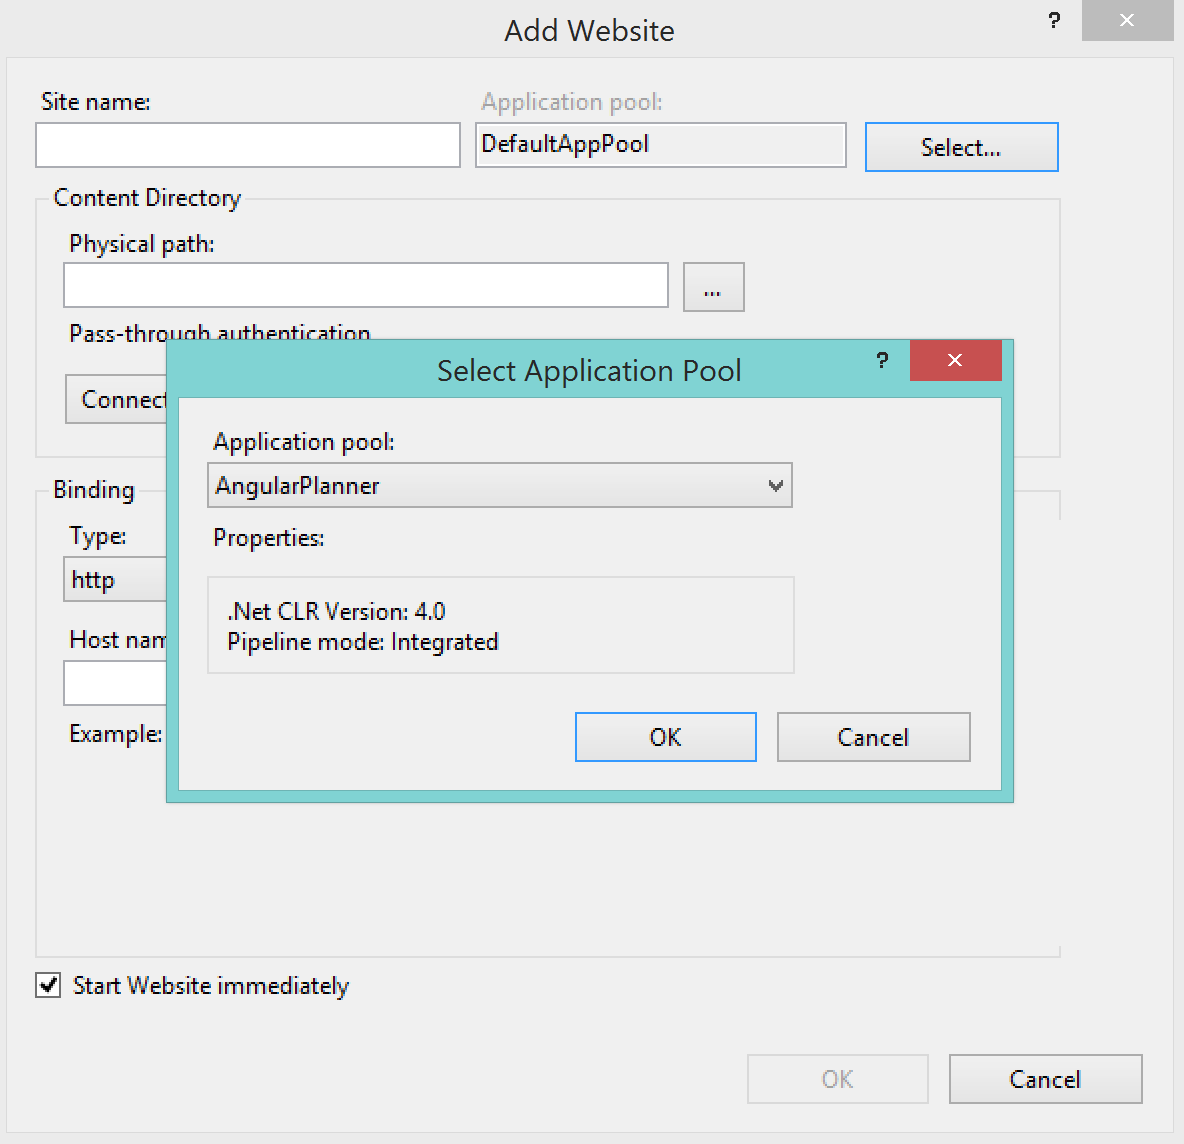
\includegraphics[scale=0.35]{images/install9.png}
  \caption{Wybór puli}
\end{figure}
\par Pozostałe pola wypełnić jak poniżej. Jedynie można zmienić ścieżkę do aplikacji. Zatwierdzić wszystko przyciskiem OK.
\begin{figure}[H]
  \centering
  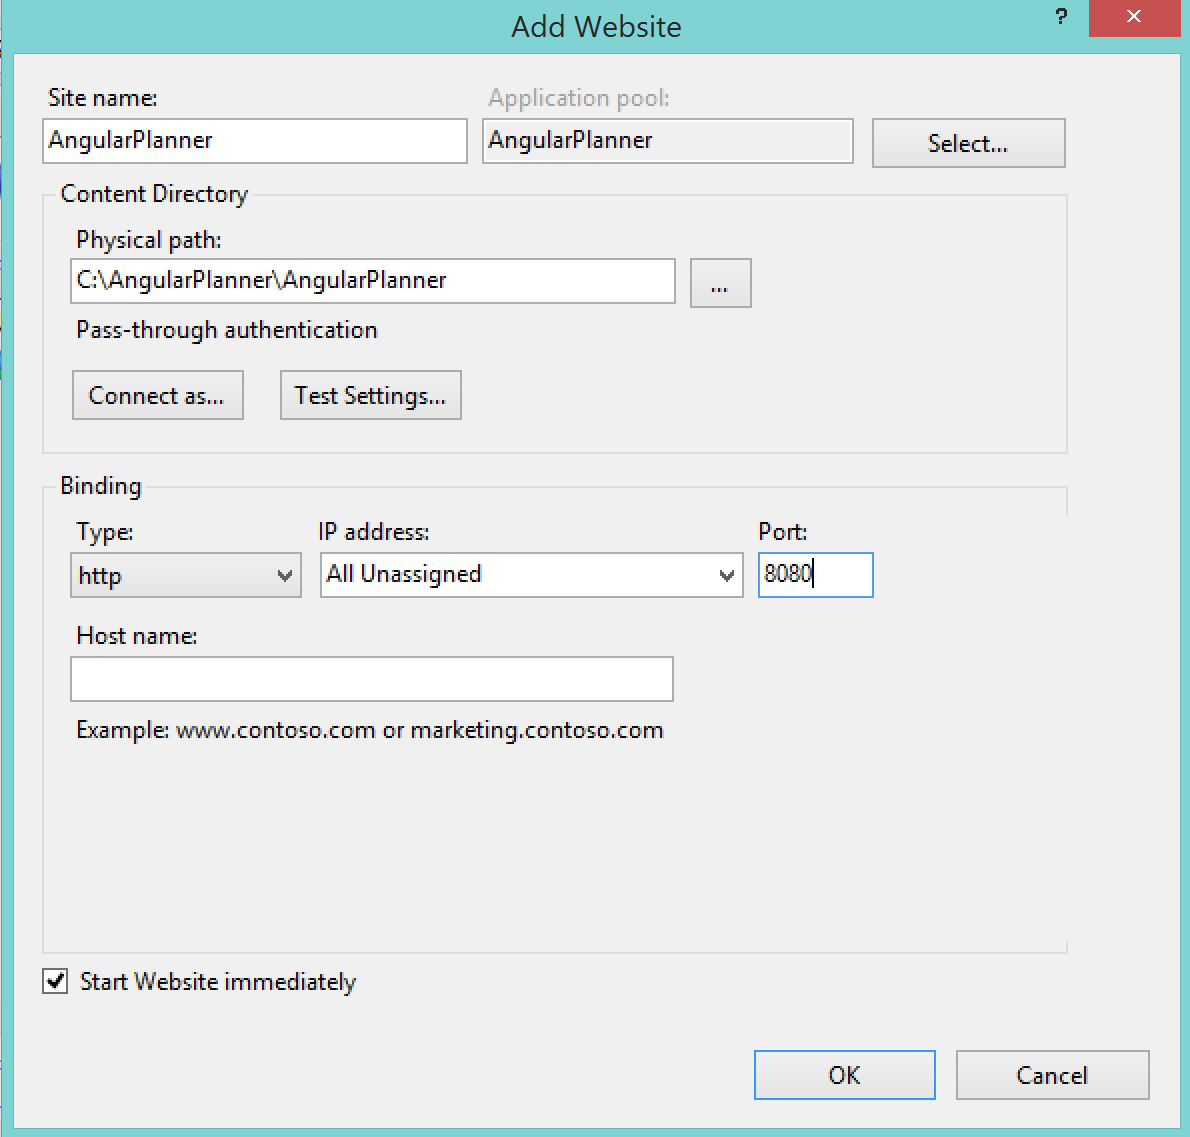
\includegraphics[scale=0.35]{images/install10.png}
  \caption{Uzupełnianie danych}
\end{figure}
\par Przejść do \verb|Application Pools| wybrać pulę \verb|AngularPlanner| i w prawej kolumnie kliknąć \verb|Start|.
\begin{figure}[H]
  \centering
  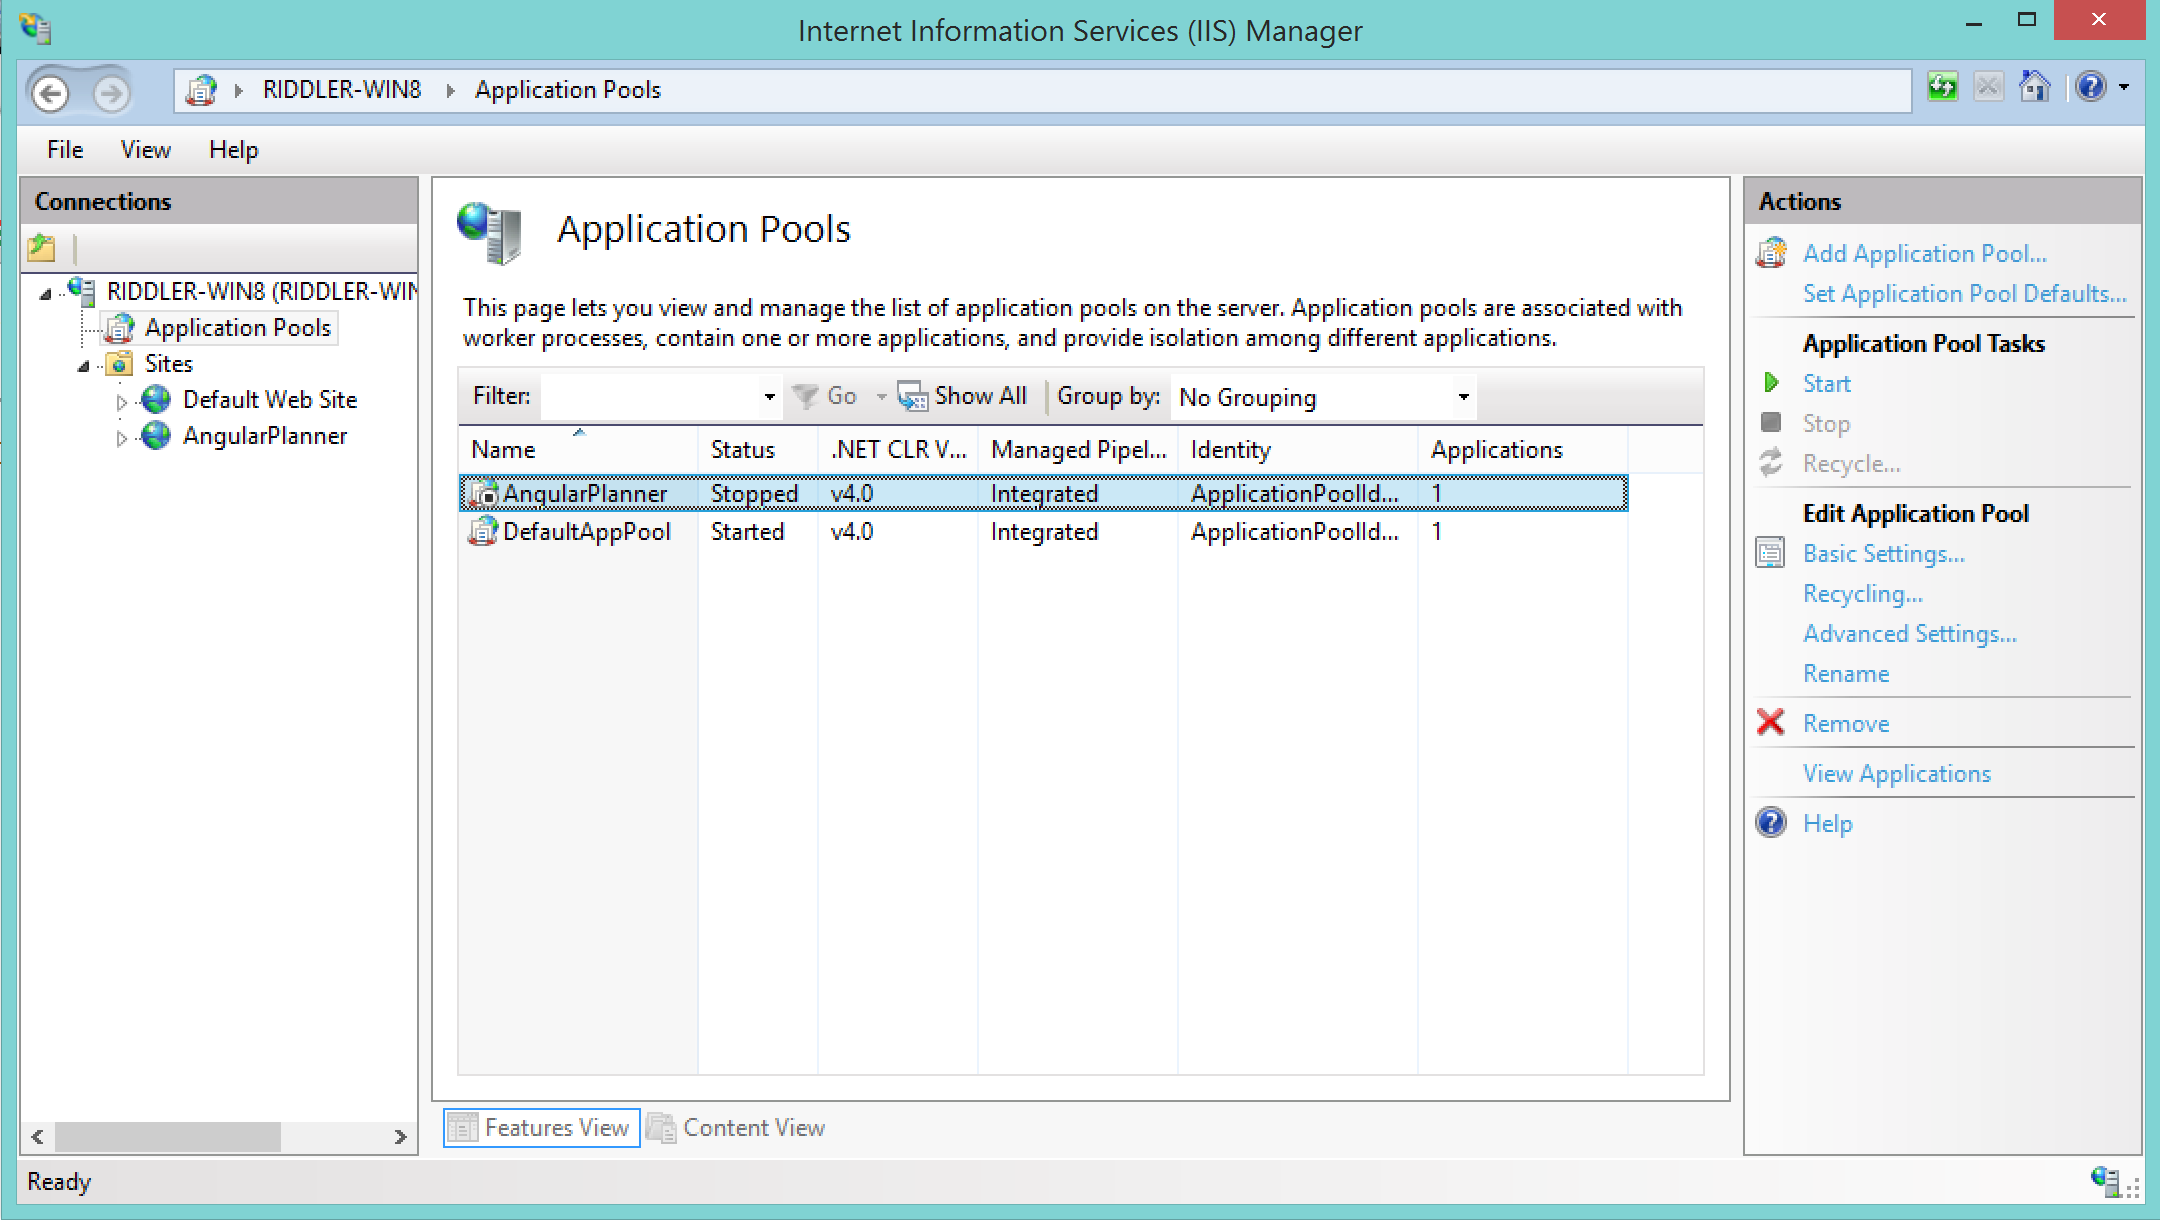
\includegraphics[scale=0.35]{images/install11.png}
  \caption{Uruchamianie puli}
\end{figure}

\section*{Podsumowanie}
Podczas prac implementacyjnych większość założonych funkcjonalności zostało wykonanych. Nie udało się zrobić zakładki ze statystykami wszystkich użytkowników systemie. Oczywiście byłyby one bardzo ogólne, aby dbać o ochronę danych klientów. Także możnaby było rozwinąć funkcję przewidywania wydatków o precyzyjniejsze i bardziej skomplikowane algorytmy. Jeden z najważniejszych celi został osiągnięty, a było nim uproszczenie wszelkich operacji, aby użytkownik bez instrukcji użytkowania wiedział do czego służą funkcje i jak je obsłużyć.
\par Najwięcej problemów było z biblioteką AngularJS i stworzeniem mechanizmu logowania w tej technologii. Biblioteka ta oferuje bardzo dużo funkcjonalności w prosty sposób, lecz dopiero po dłuższym użytkowaniu. Dla początkujących użytkowników jest ciężka w rozumieniu. Logowanie także nie jest prostą sprawą, ponieważ mało jest materiałów w Internecie i literaturze o logowaniu tokenowym.

%%%%%%%%%%%%%%%%%%%%%%%%%%%%%%%%%%%%%%%%%%%%%%%%%%%%%%%%%%%%%%%%%%%%%%%%%%%%%%
%%%%%%%%%%%%%%%%%%%%%%%%%%%%%%% BIBLIOGRAFIA %%%%%%%%%%%%%%%%%%%%%%%%%%%%%%%%%
%%%%%%%%%%%%%%%%%%%%%%%%%%%%%%%%%%%%%%%%%%%%%%%%%%%%%%%%%%%%%%%%%%%%%%%%%%%%%%


\bibliography{bibl}
\bibliographystyle{plain}

\end{document}
